\section{Results}


Large number of MAPMTs from Hamamatsu (XX of H8500 type, and XXX of H12700 type) were studied using the dedicated test stand at JLab. Their performance as single photon detectors was evaluated and characterized in conditions close to their future operations in the CLAS12 RICH detector.


Parameters of the single photoelectron response function of every pixel were extracted using the SPE spectra approximations in our mathematical model, modified to take into account the effects of the signal cross-talk between the neighboring pixels. The stability and consistency of the parameter values measured in different conditions of illumination and at different applied high voltages allows to characterize the intrinsic features of every pixel, independent on the measurement conditions. Absolute quantum efficiency and electronic gain of every channel, as well as the set of parameters describing variable shapes of the SPE functions were measured.


The parameter database accumulated as the result of this work may be used for the selection of the PSPMTs for installation in the RICH detector, and for the optimization of the future run parameters, such as the tube placement selection, setting the values of operating high voltage, electronics gains and thresholds in the detector.


The data also provide the opportunity to evaluate the spread of such parameters in the mass production of the PSPMT devices as the channel gains, quantum efficiencies, SPE spectral shapes, parameters of the cross-talk, - across the face of each tube, and across the whole set. The results show that the quality of PSPMT mass production at Hamamatsu is high and satisfies our needs in the good quality single photoelectron detection.




\begin{figure*}[t]
	\centering
	\begin{subfigure}[c]{0.42\linewidth}
		\centering
		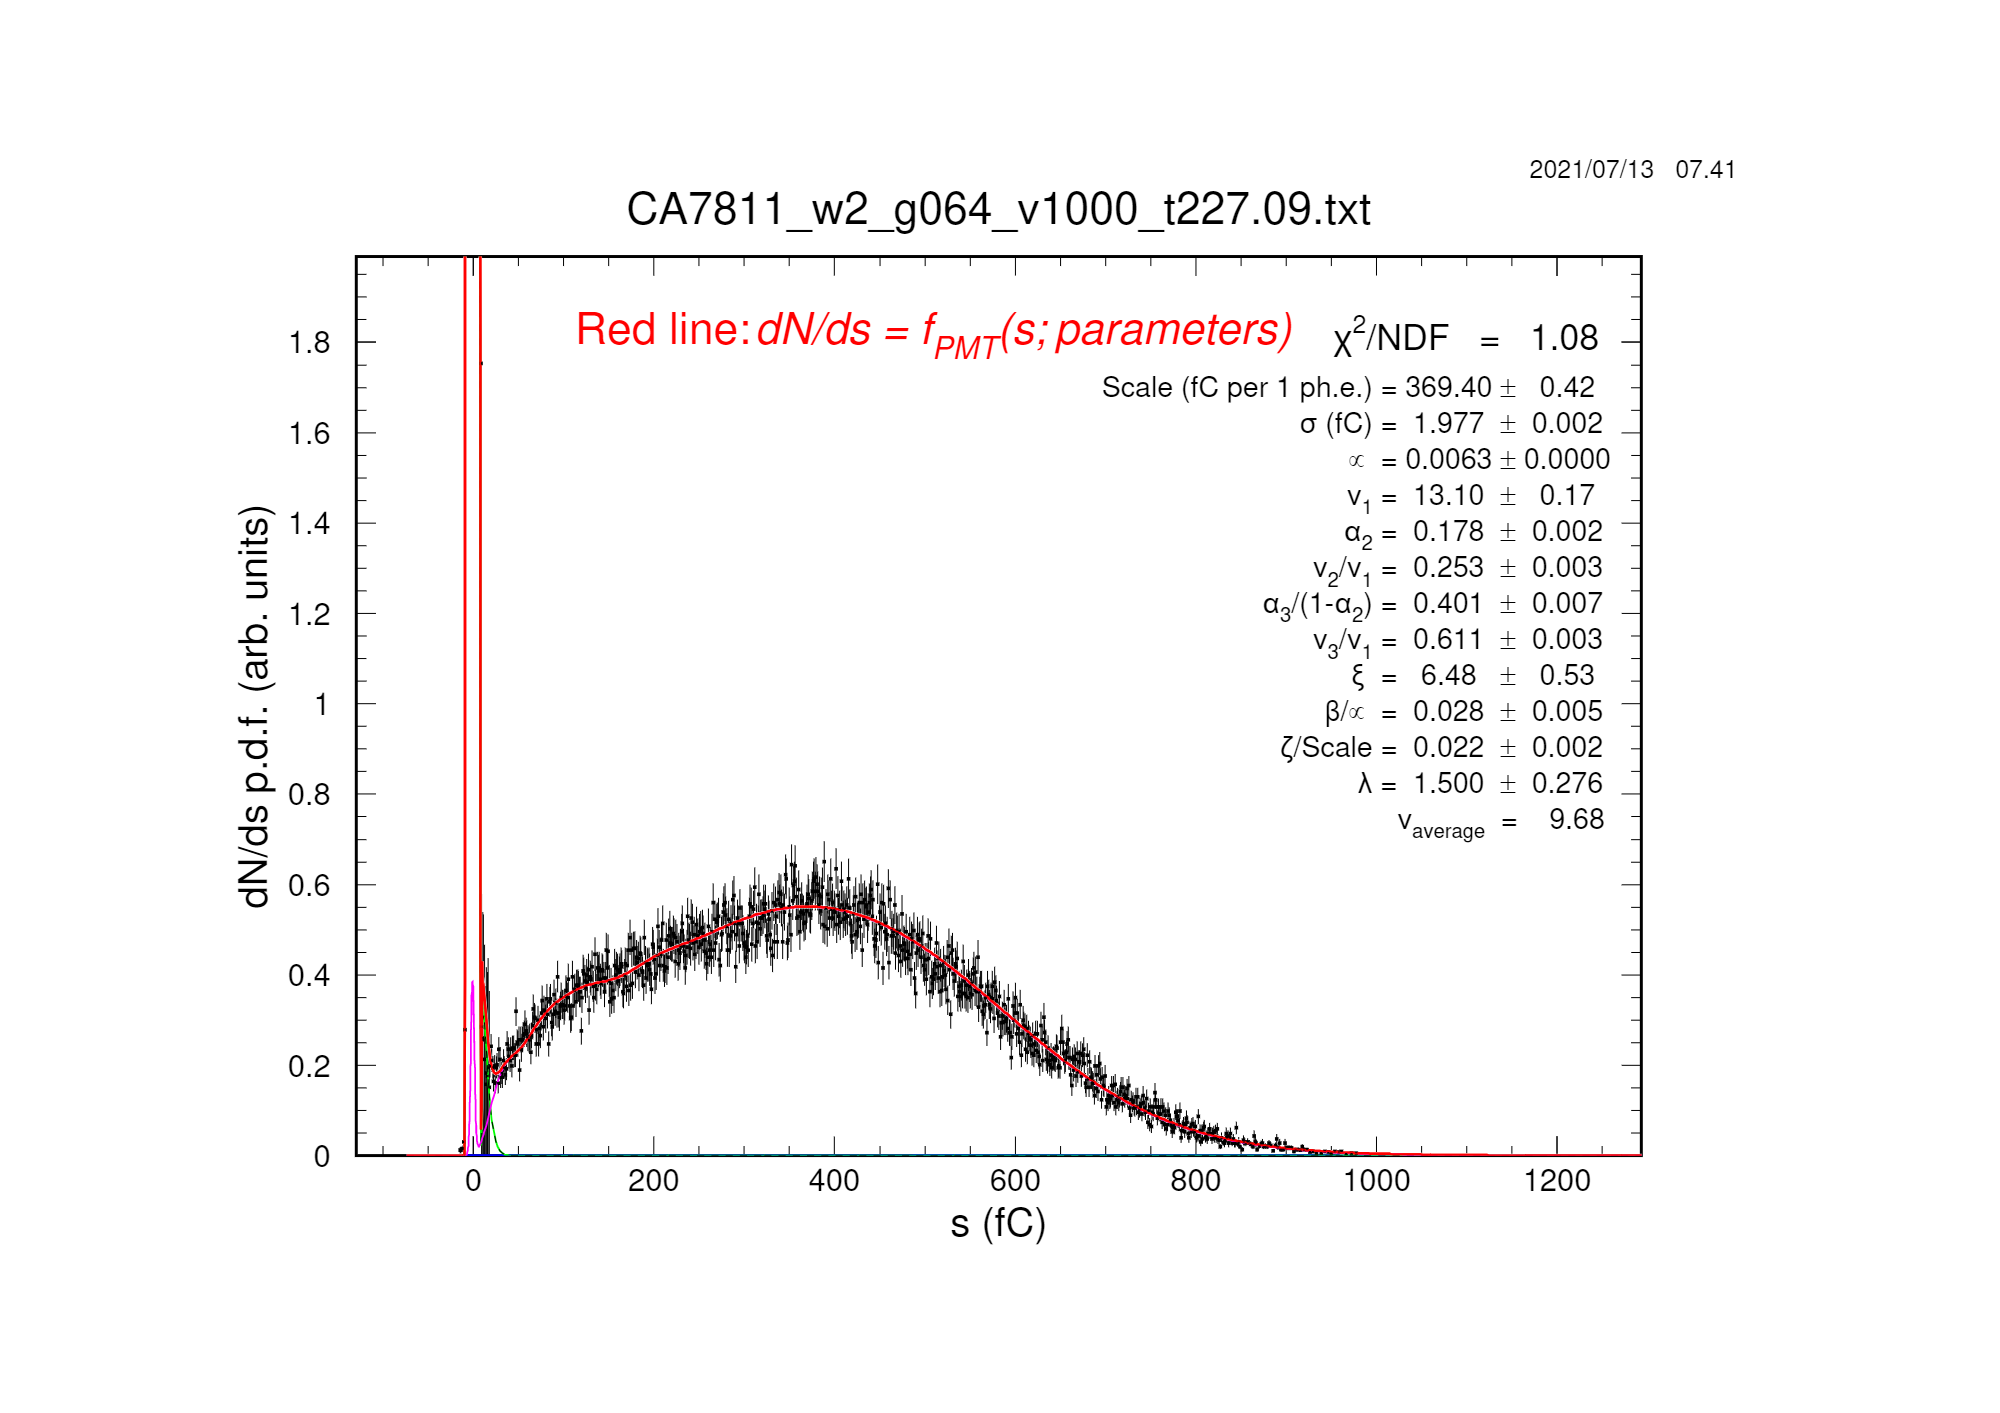
\includegraphics[width=\linewidth, trim={6cm 6cm 80mm 85mm},clip]{figures/pavel_temp/CA7811_w2_g064_v1000_3mm.09.png}
		\vspace{0mm}
	\end{subfigure}%%
	\begin{subfigure}[c]{0.42\linewidth}
		\centering
		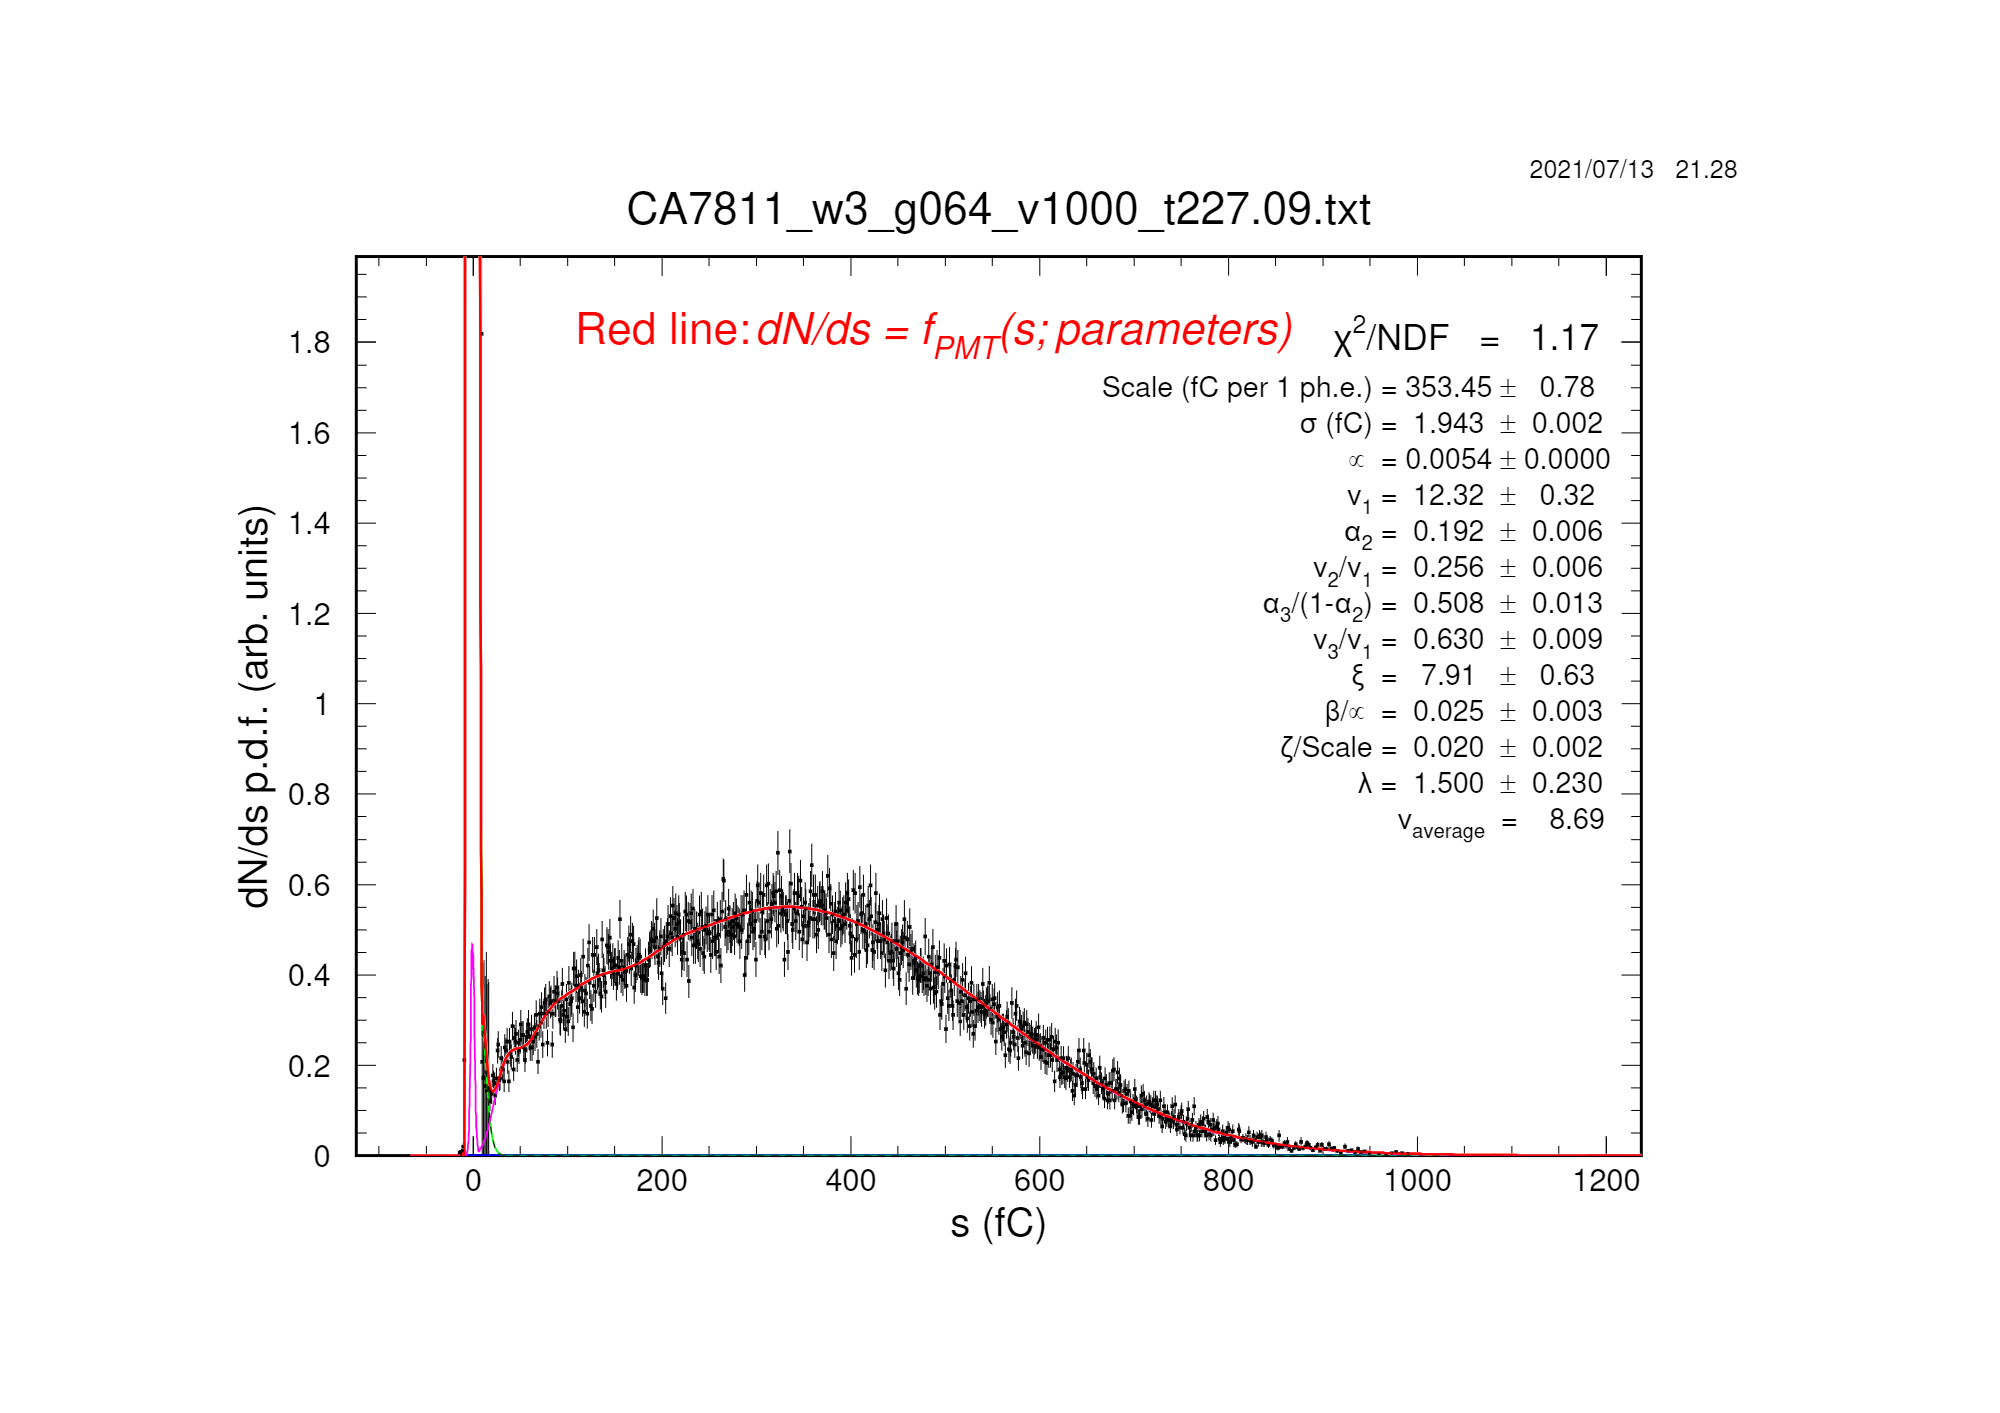
\includegraphics[width=\linewidth, trim={80mm 6cm 6cm 85mm},clip]{figures/pavel_temp/CA7811_w3_g064_v1000_cln.09.png}
		\vspace{0mm}
	\end{subfigure}%%
	\vspace{0mm}
	\begin{subfigure}[c]{0.42\linewidth}
		\centering
		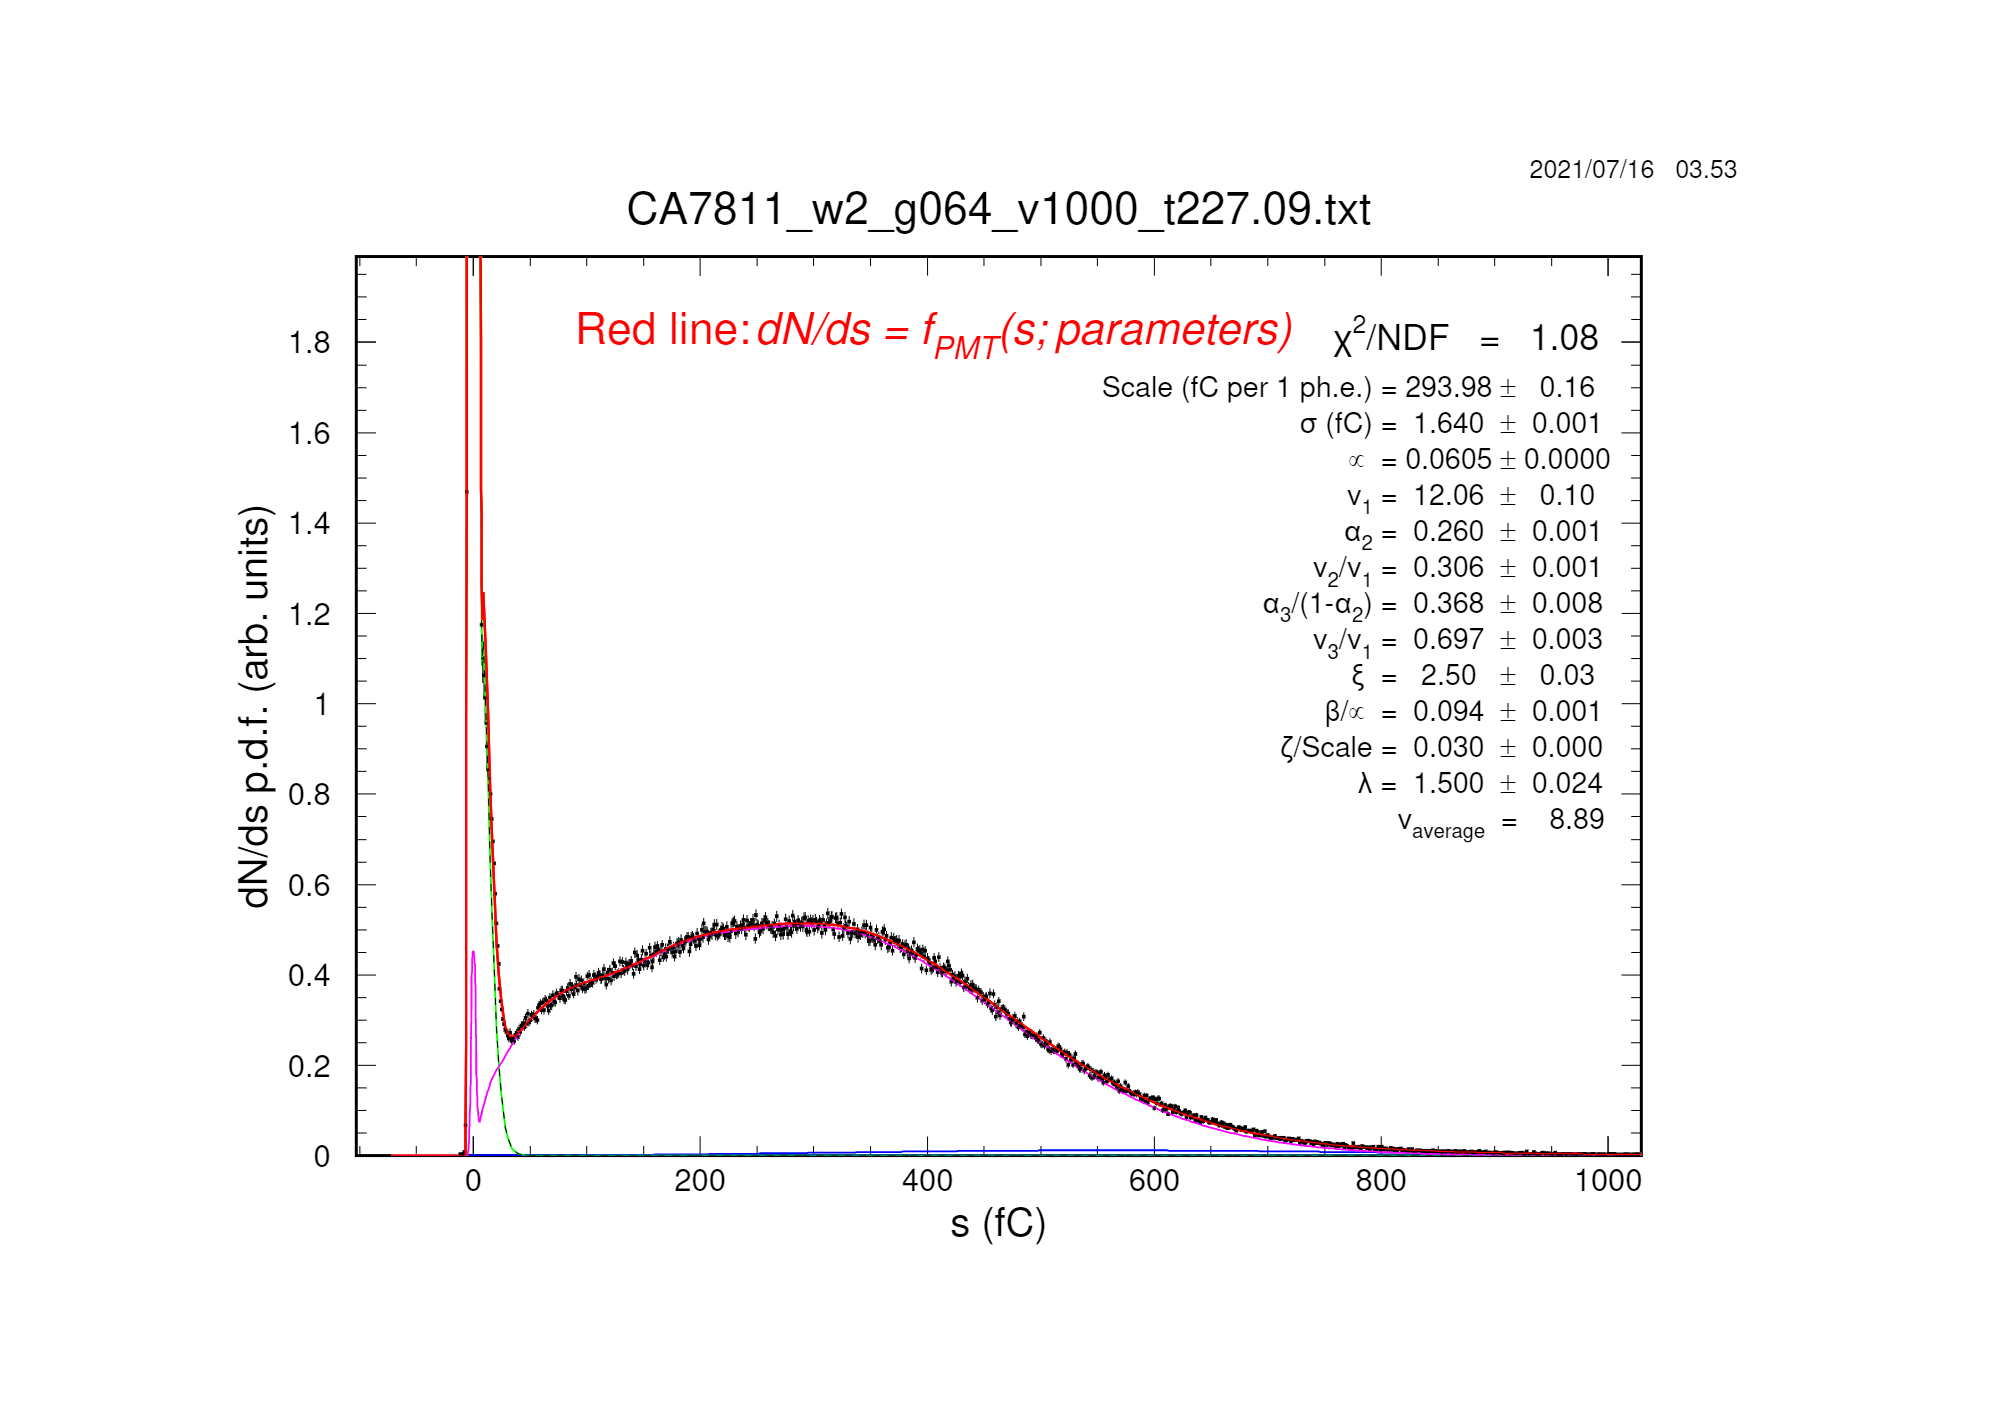
\includegraphics[width=\linewidth, trim={6cm 6cm 80mm 85mm},clip]{figures/pavel_temp/CA7811_w2_g064_v1000_6mm.09.png}
		\vspace{0mm}
	\end{subfigure}%%
	\begin{subfigure}[c]{0.42\linewidth}
		\centering
		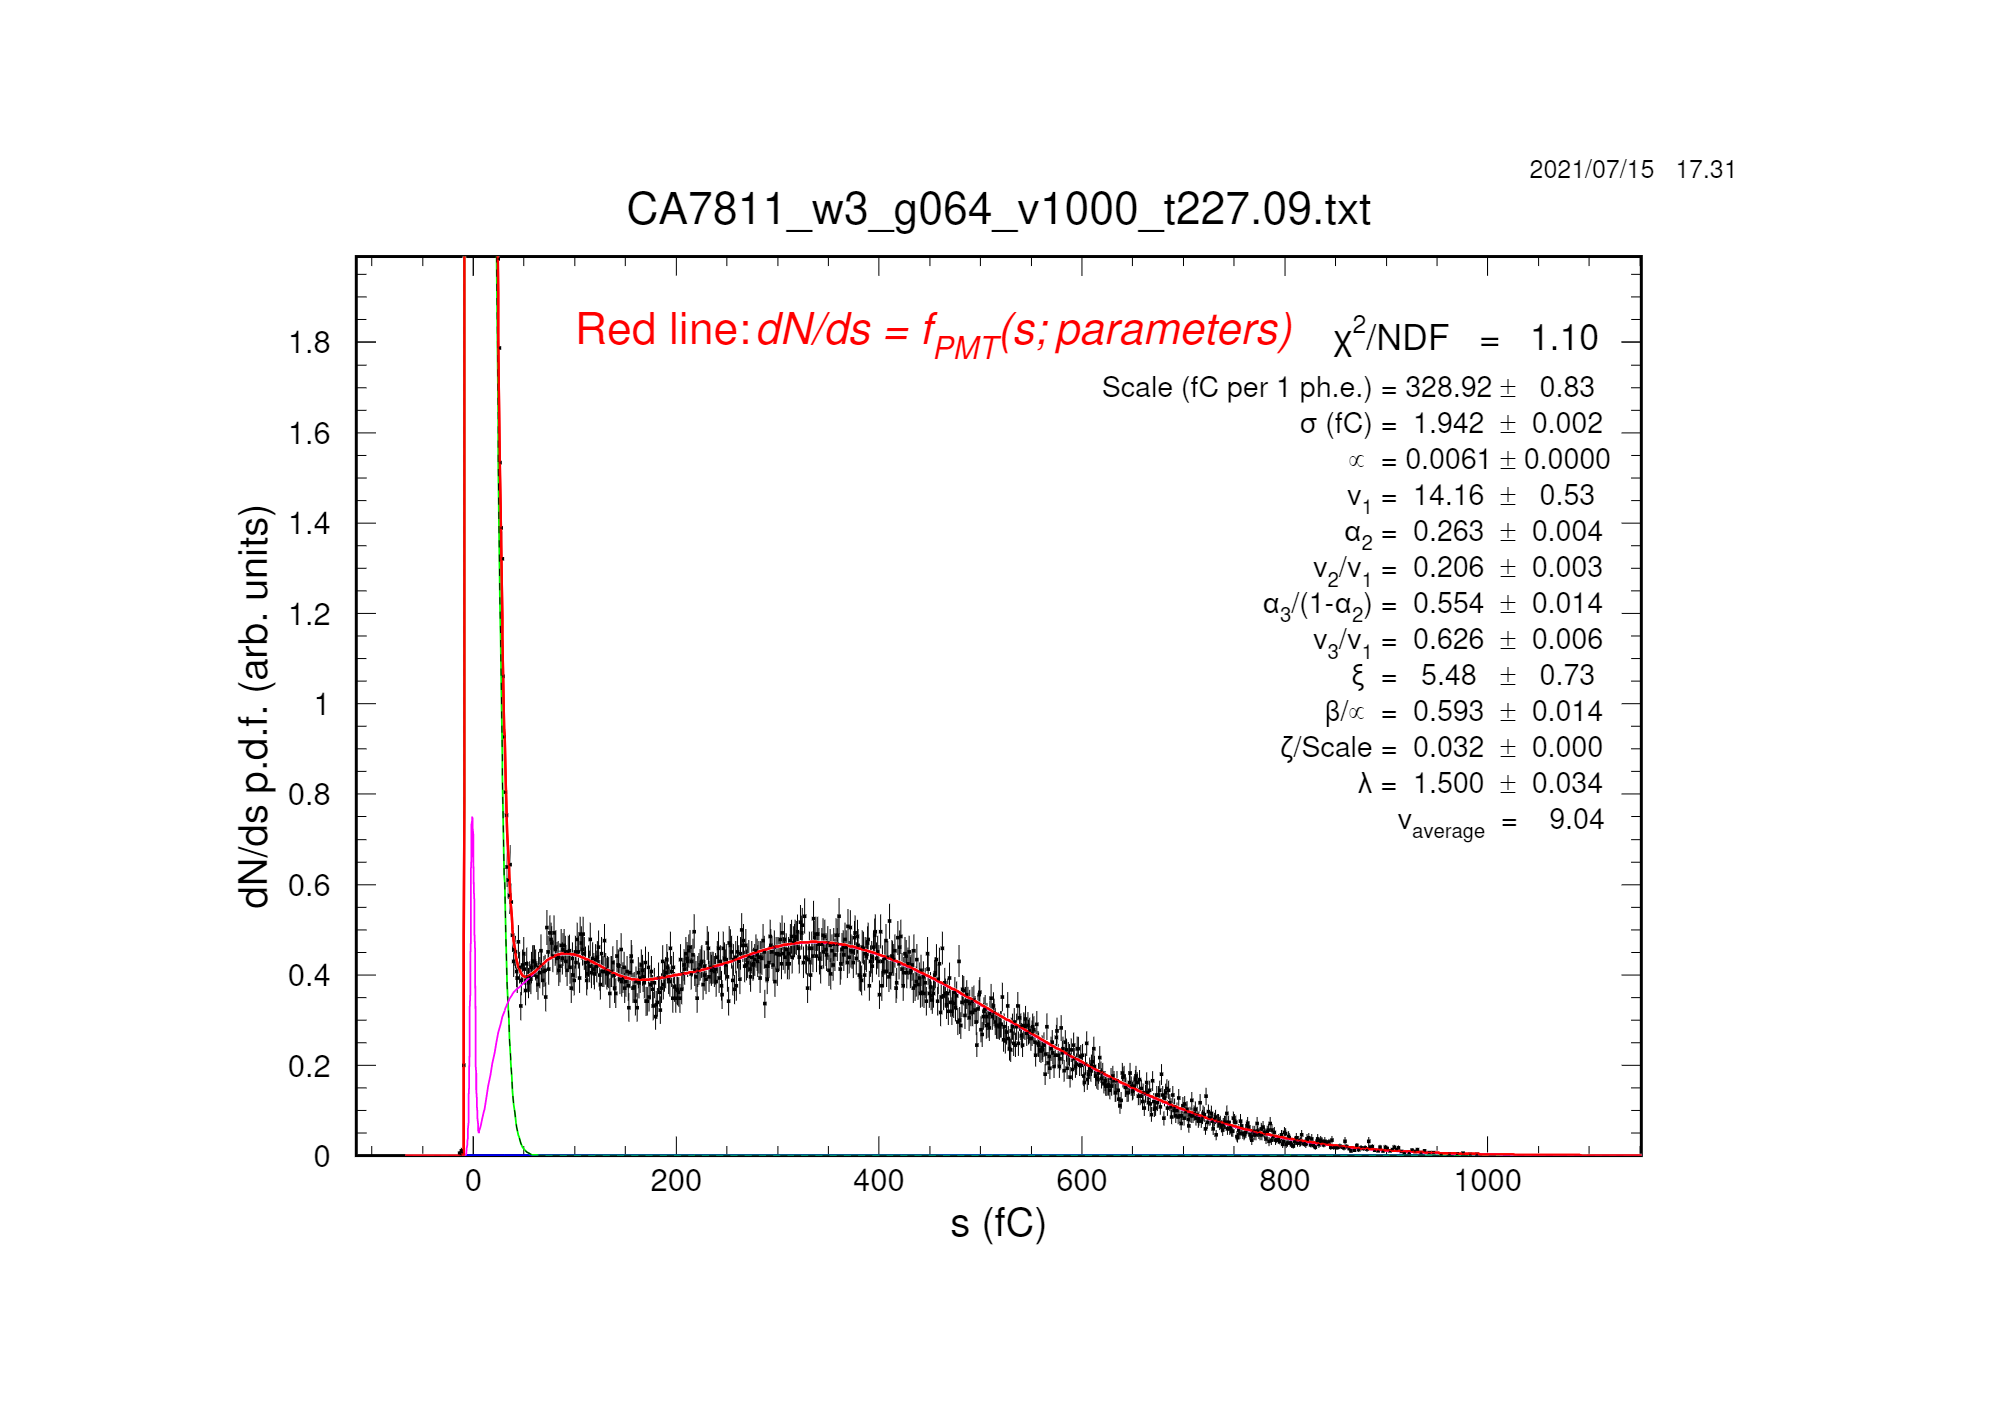
\includegraphics[width=\linewidth, trim={80mm 6cm 6cm 85mm},clip]{figures/pavel_temp/CA7811_w3_g064_v1000_raw.09.png}
		\vspace{0mm}
	\end{subfigure}%%
	\caption{SPE probability distributions for PMT CA7811 (H8500), pixel 9, at HV = 1000 V. Top Left: 3mm mask. Bottom left: 6mm mask. Top right: run with full PMT face open, cross-talk events removed by the correlation analysis. Bottom right: run with full PMT face open, the contribution to the spectrum from the cross-talk events is approximated and parameterized by the analysis algorithm. The cross talk effects are too wide to be approximated correctly.}
	\label{fig:CA7811_fits}
\end{figure*}

\vspace{5cm}

\begin{figure*}[b]
	\centering
	\begin{subfigure}[c]{0.42\linewidth}
		\centering
		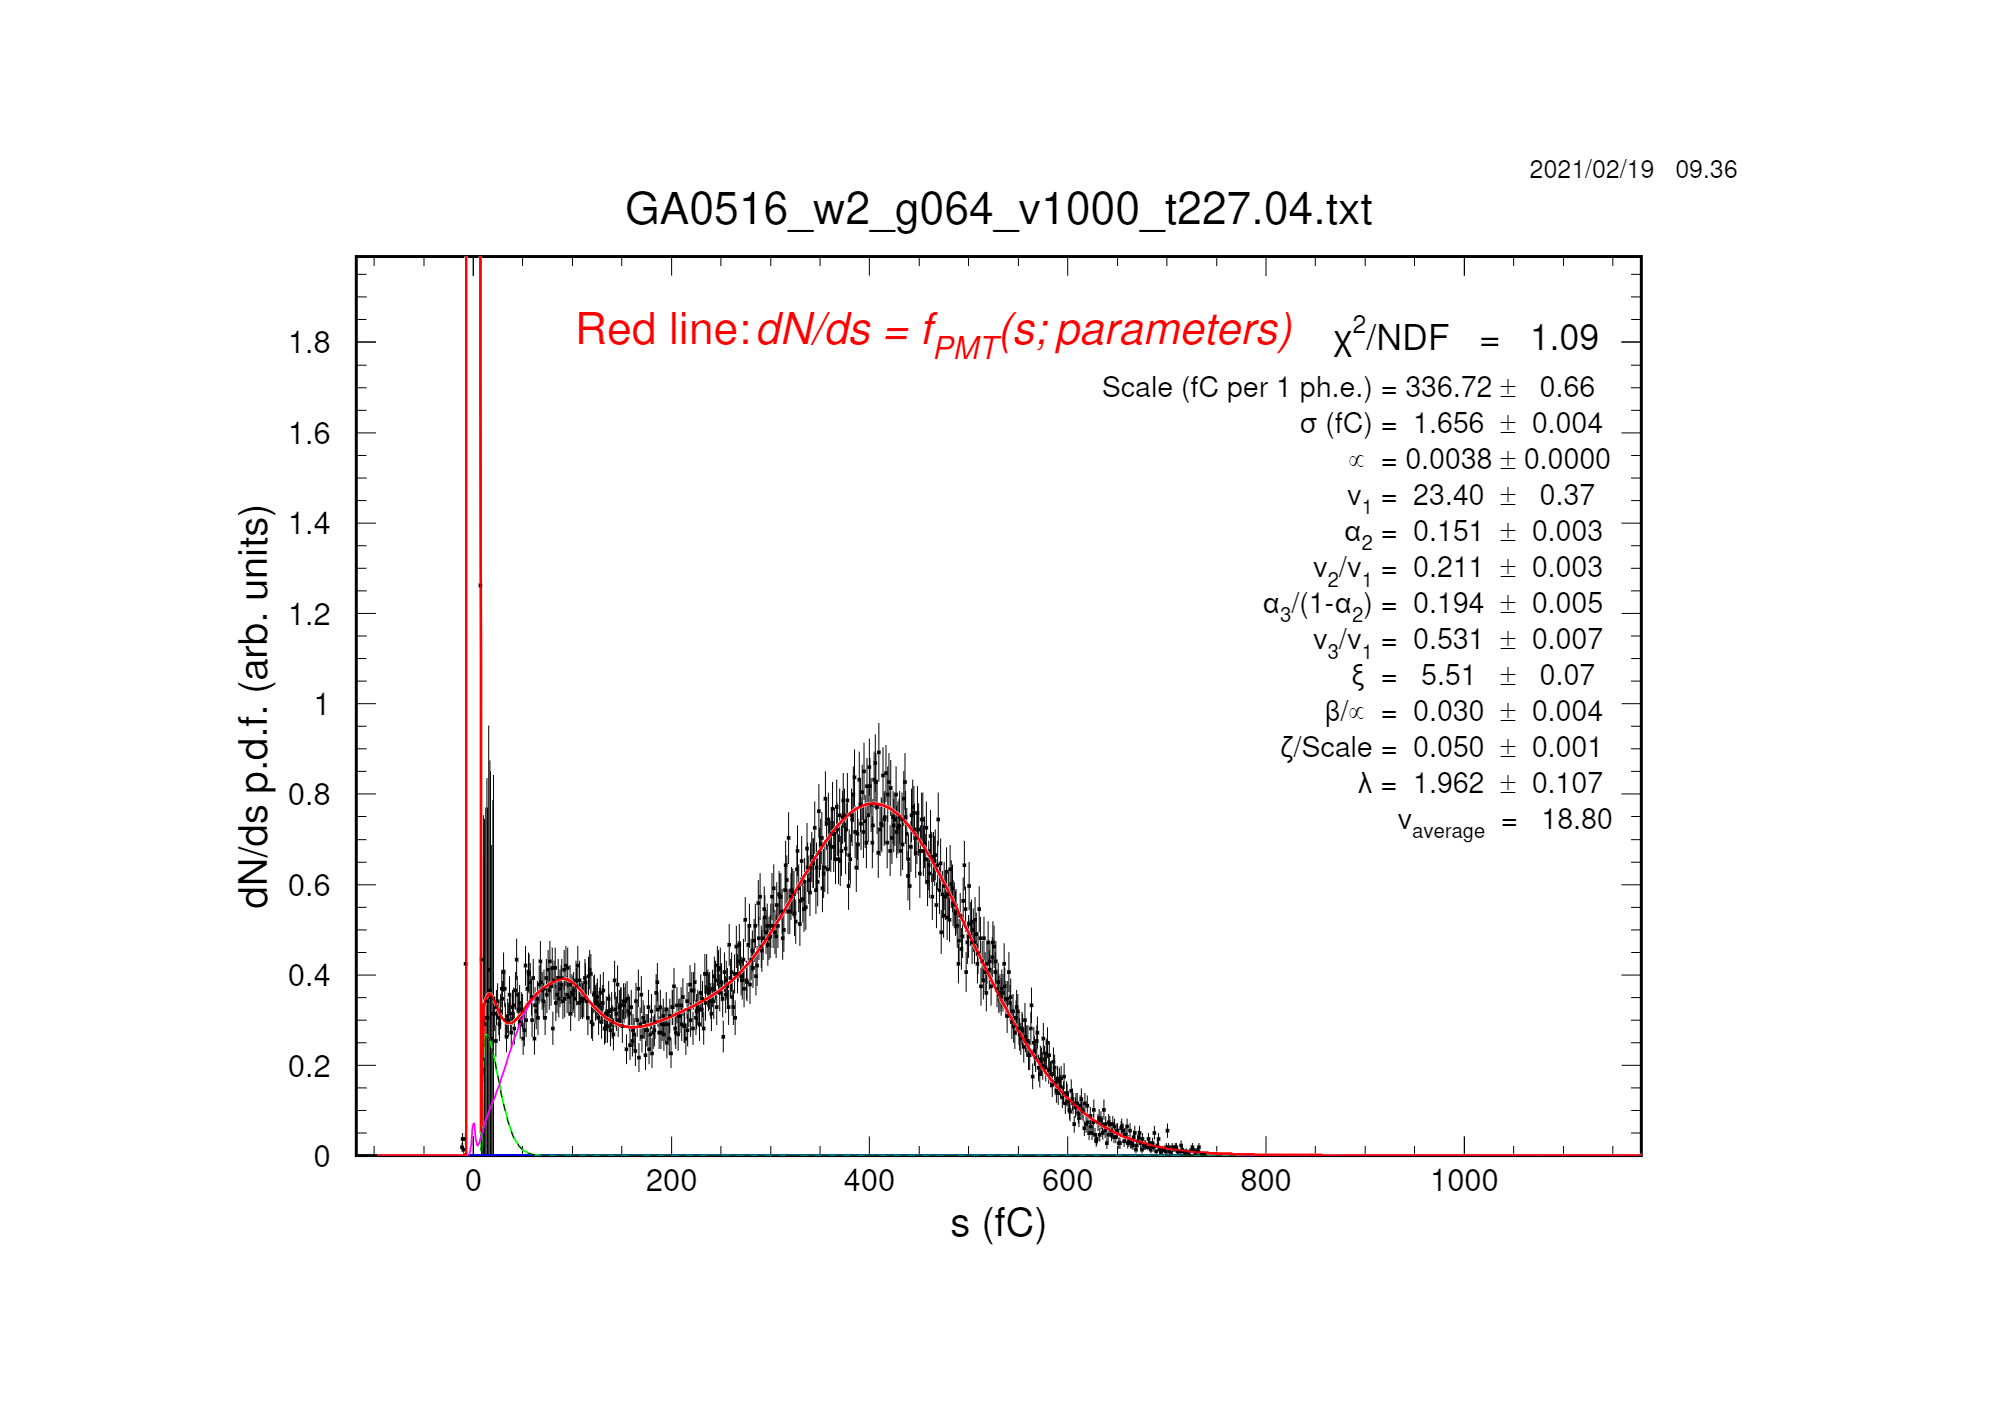
\includegraphics[width=\linewidth, trim={6cm 6cm 75mm 85mm},clip]{figures/pavel_temp/GA0516_w2_g064_v1000_3mm.04.png}
		\vspace{0mm}
	\end{subfigure}%%
	\begin{subfigure}[c]{0.42\linewidth}
		\centering
		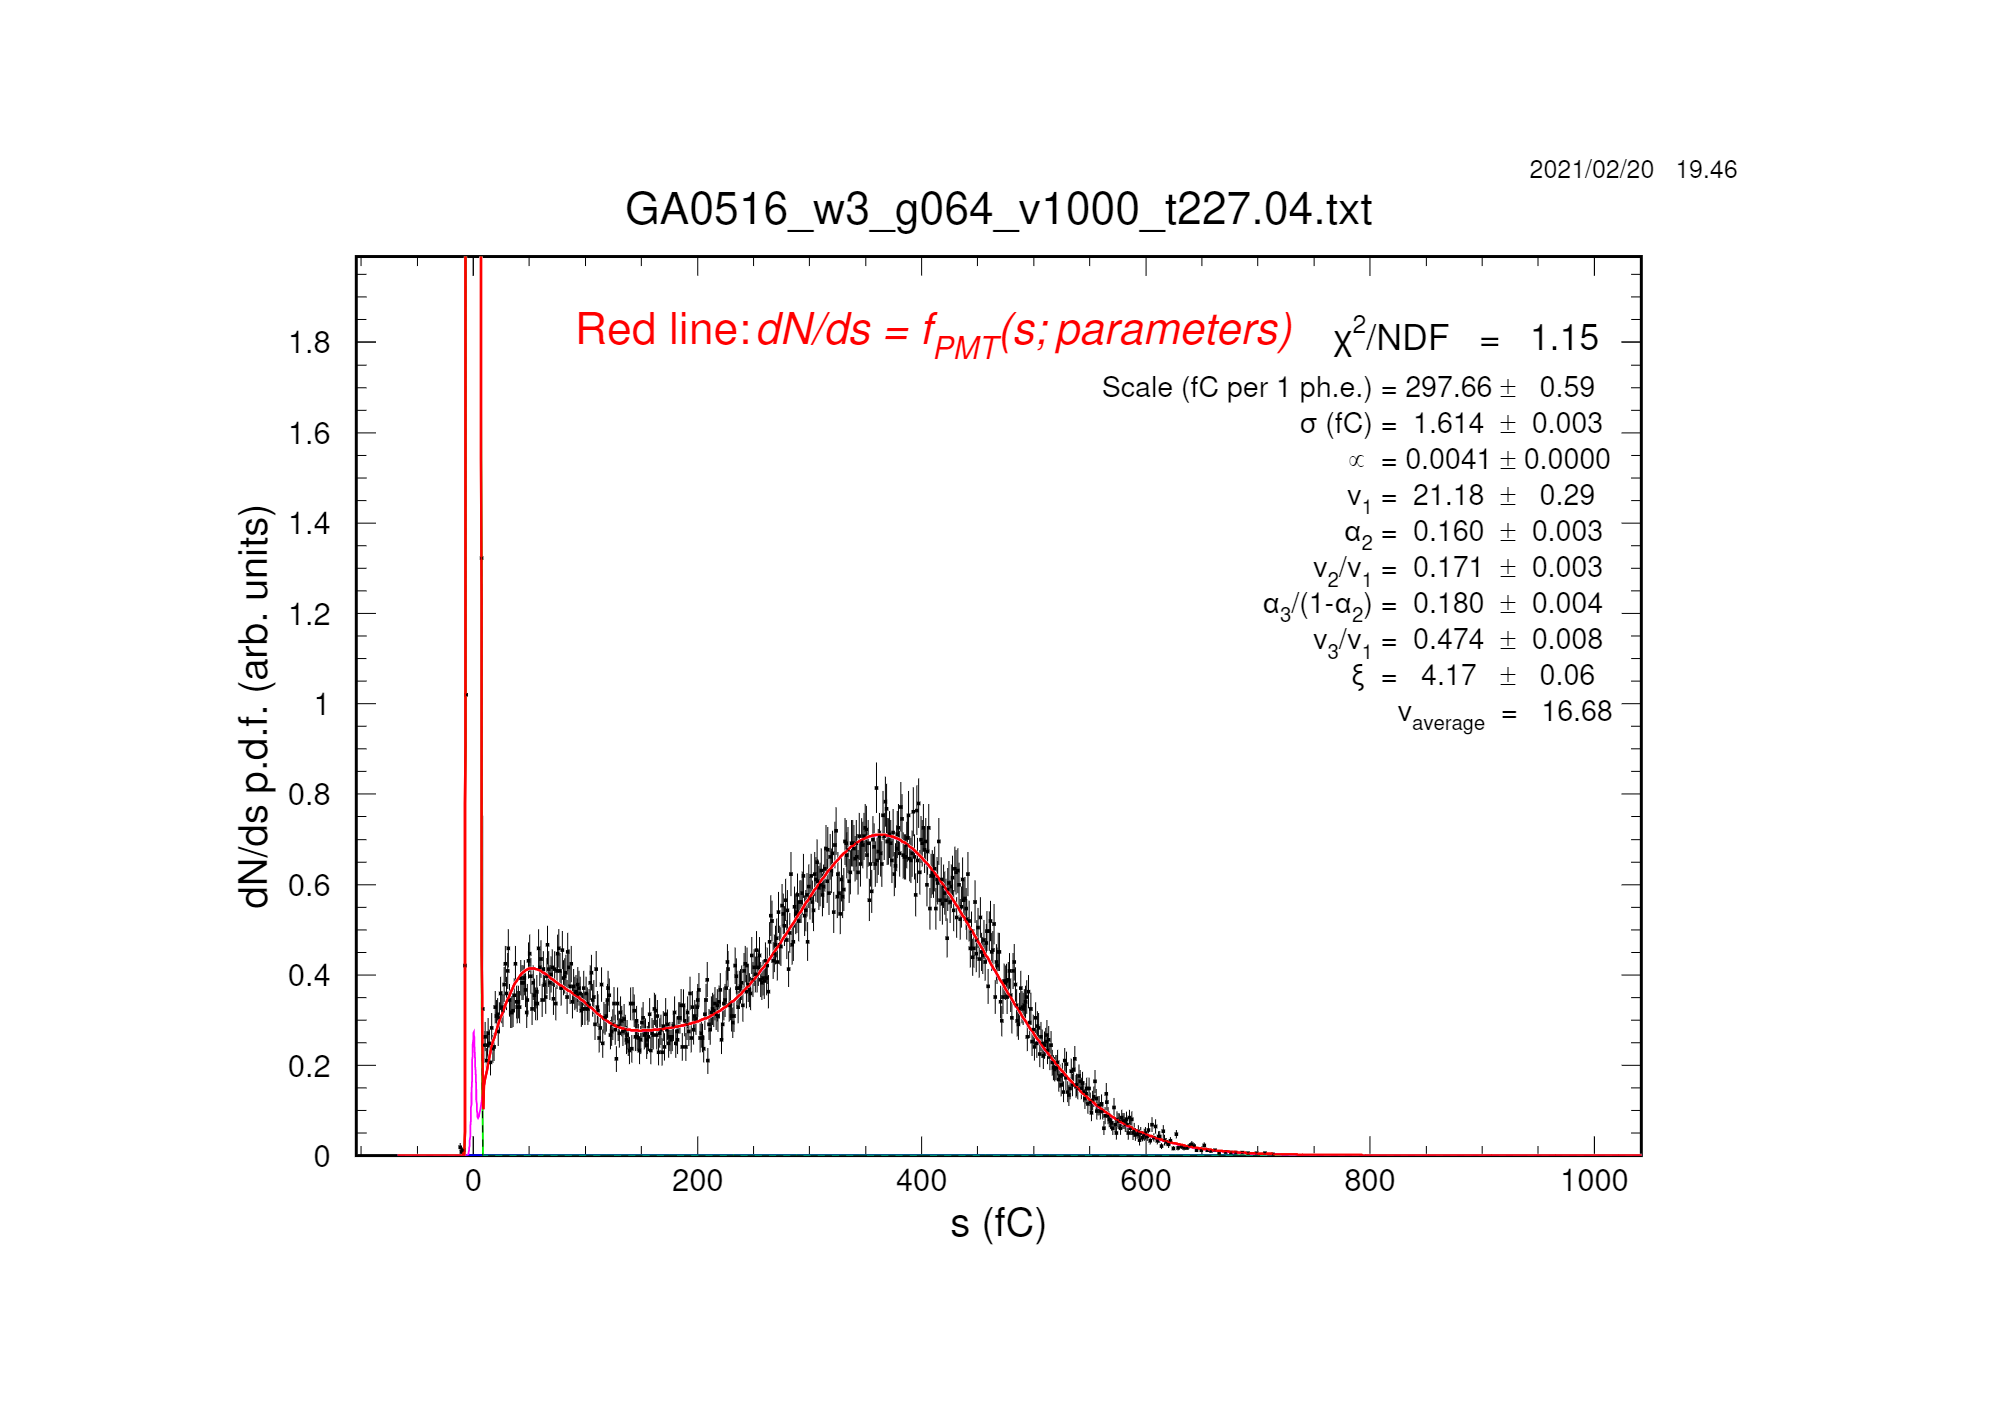
\includegraphics[width=\linewidth, trim={75mm 6cm 6cm 85mm},clip]{figures/pavel_temp/GA0516_w3_g064_v1000_cln.04.png}
		\vspace{0mm}
	\end{subfigure}%%
	\vspace{0mm}
	\begin{subfigure}[c]{0.42\linewidth}
		\centering
		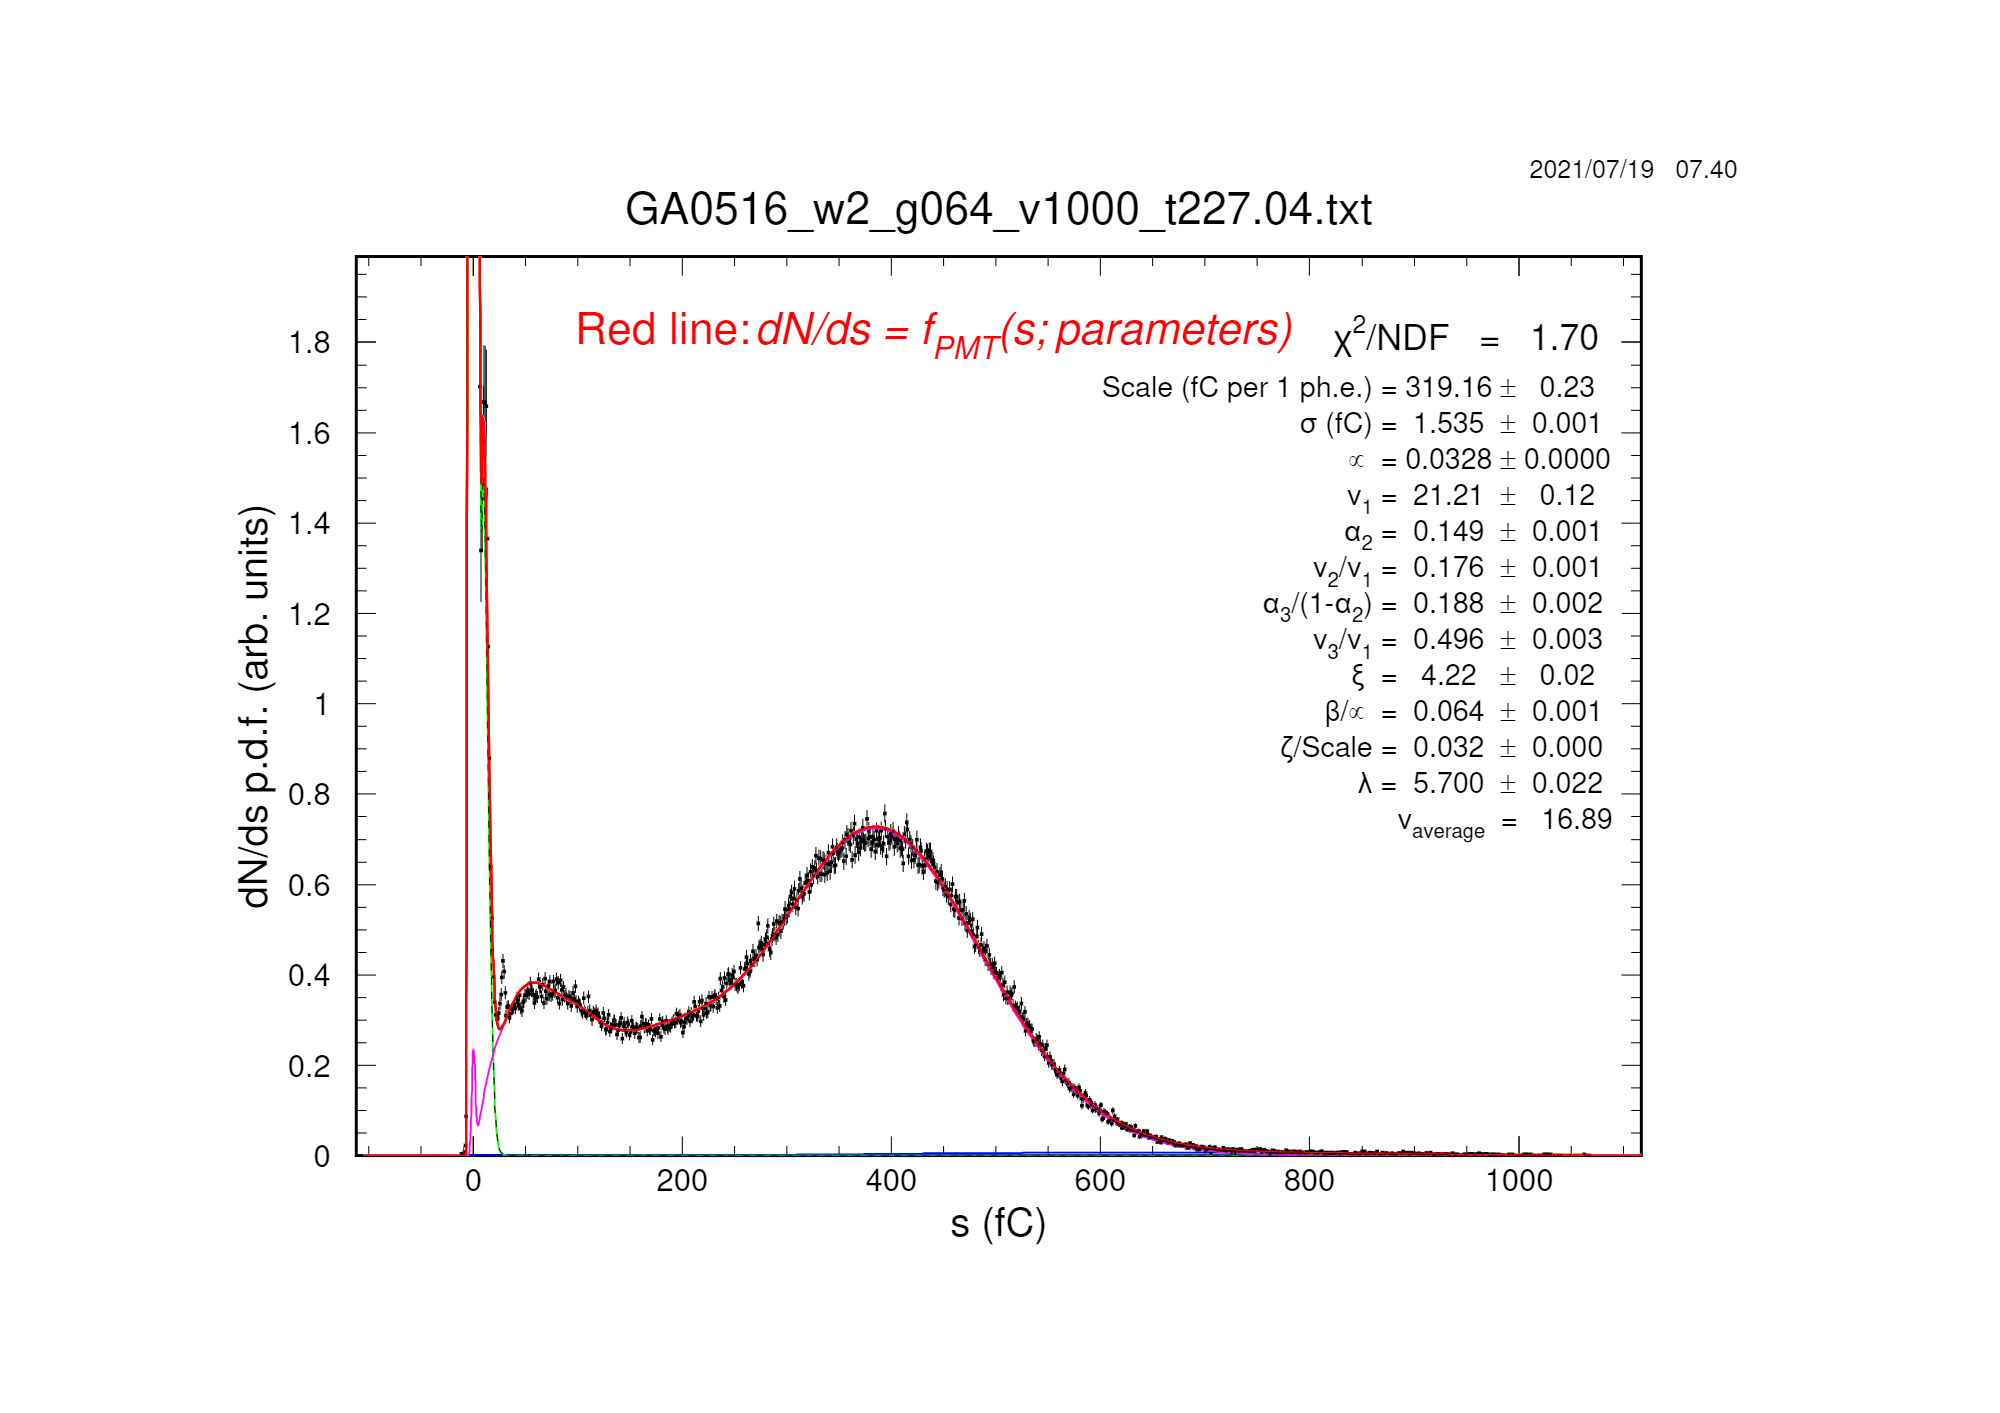
\includegraphics[width=\linewidth, trim={6cm 6cm 75mm 85mm},clip]{figures/pavel_temp/GA0516_w2_g064_v1000_6mm.04.png}
		\vspace{0mm}
	\end{subfigure}%%
	\begin{subfigure}[c]{0.42\linewidth}
		\centering
		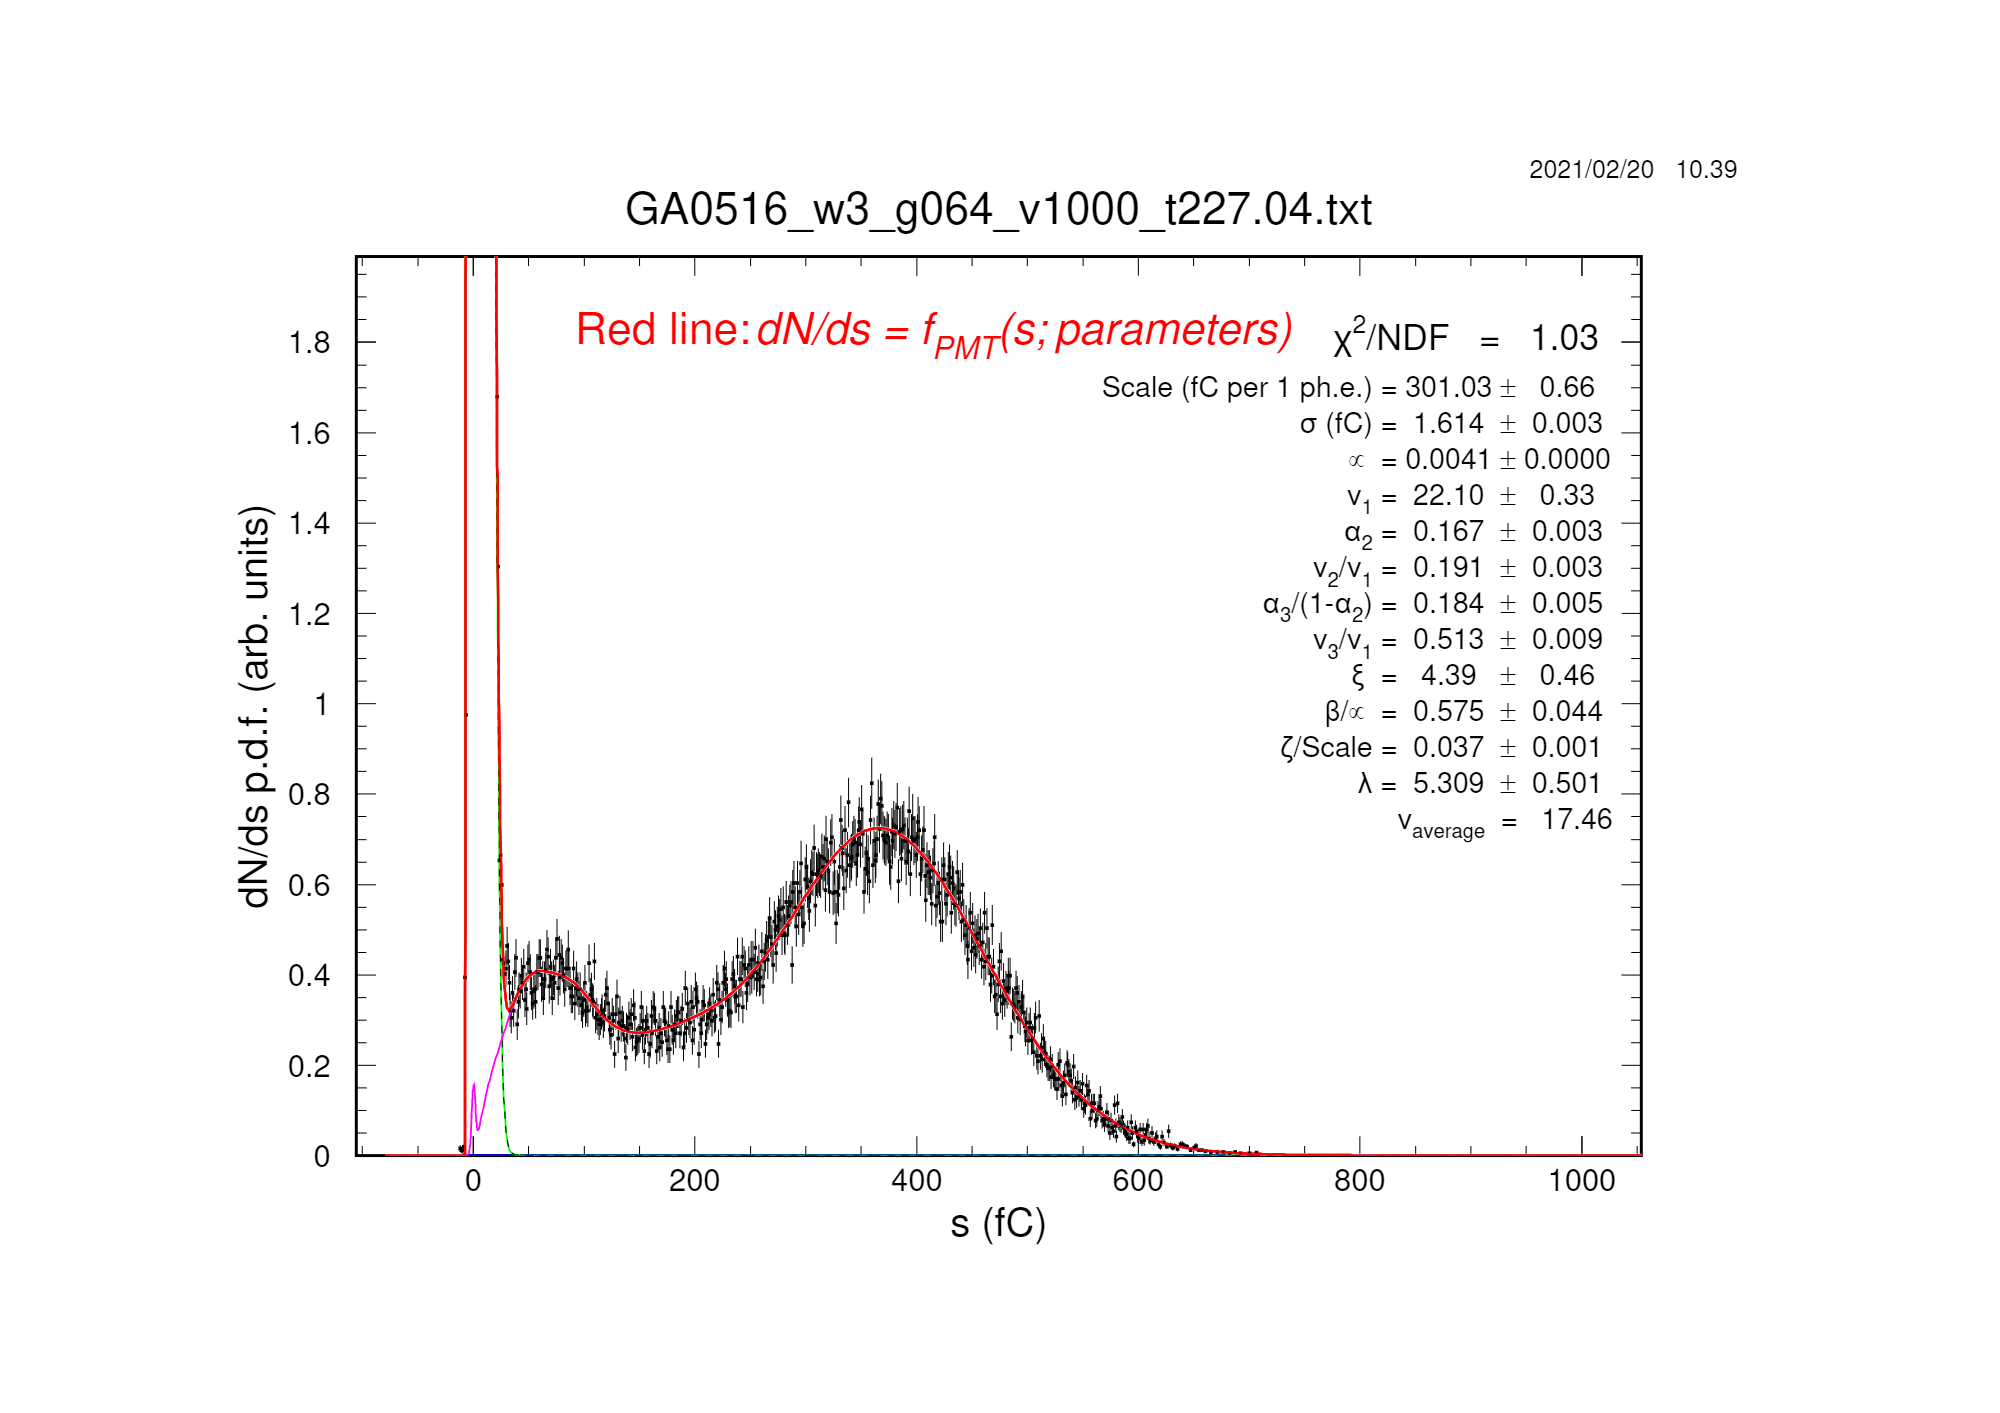
\includegraphics[width=\linewidth, trim={75mm 6cm 6cm 85mm},clip]{figures/pavel_temp/GA0516_w3_g064_v1000_raw.04.png}
		\vspace{0mm}
	\end{subfigure}%%
	\caption{SPE probability distributions for PMT GA0516 (H12700), pixel 9, at HV = 1000 V. Top Left: 3mm mask. Bottom left: 6mm mask. Top right: run with full PMT face open, cross-talk events removed by the correlation analysis. Bottom right: run with full PMT face open, the contribution to the spectrum from the cross-talk events is approximated and parameterized by the analysis algorithm.}
	\label{fig:GA0516_fits}
\end{figure*}


\begin{figure*}[b]
	\centering
	\begin{subfigure}[c]{0.42\linewidth}
		\centering
		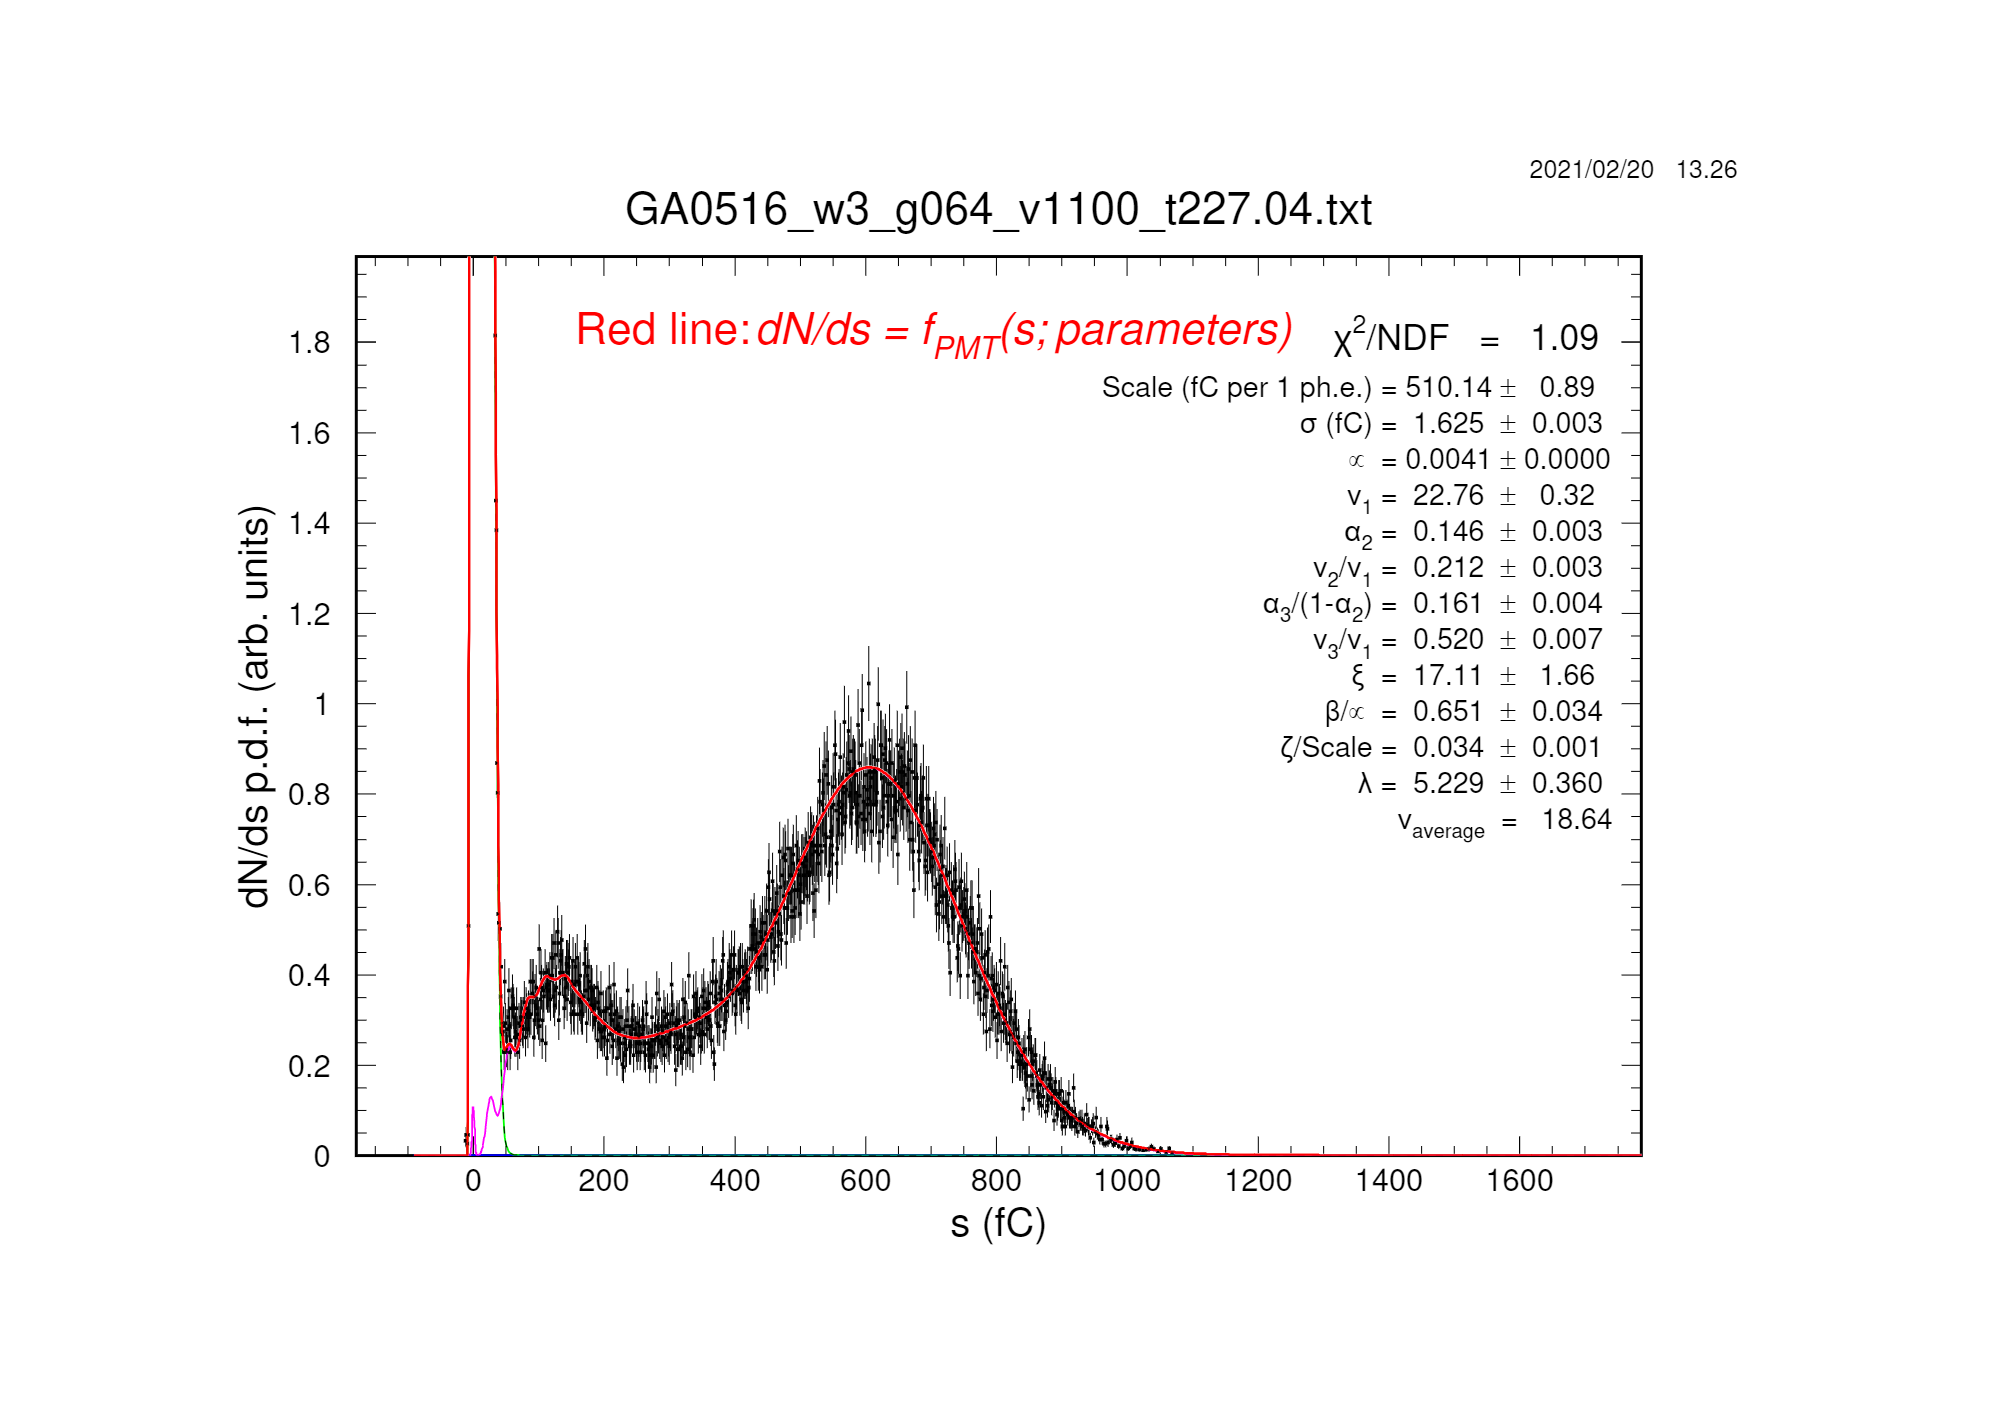
\includegraphics[width=\linewidth, trim={6cm 6cm 75mm 85mm},clip]{figures/GA0516_w2_g064_v1100_3mm.04.png}
		\vspace{0mm}
	\end{subfigure}%%
	\begin{subfigure}[c]{0.42\linewidth}
		\centering
		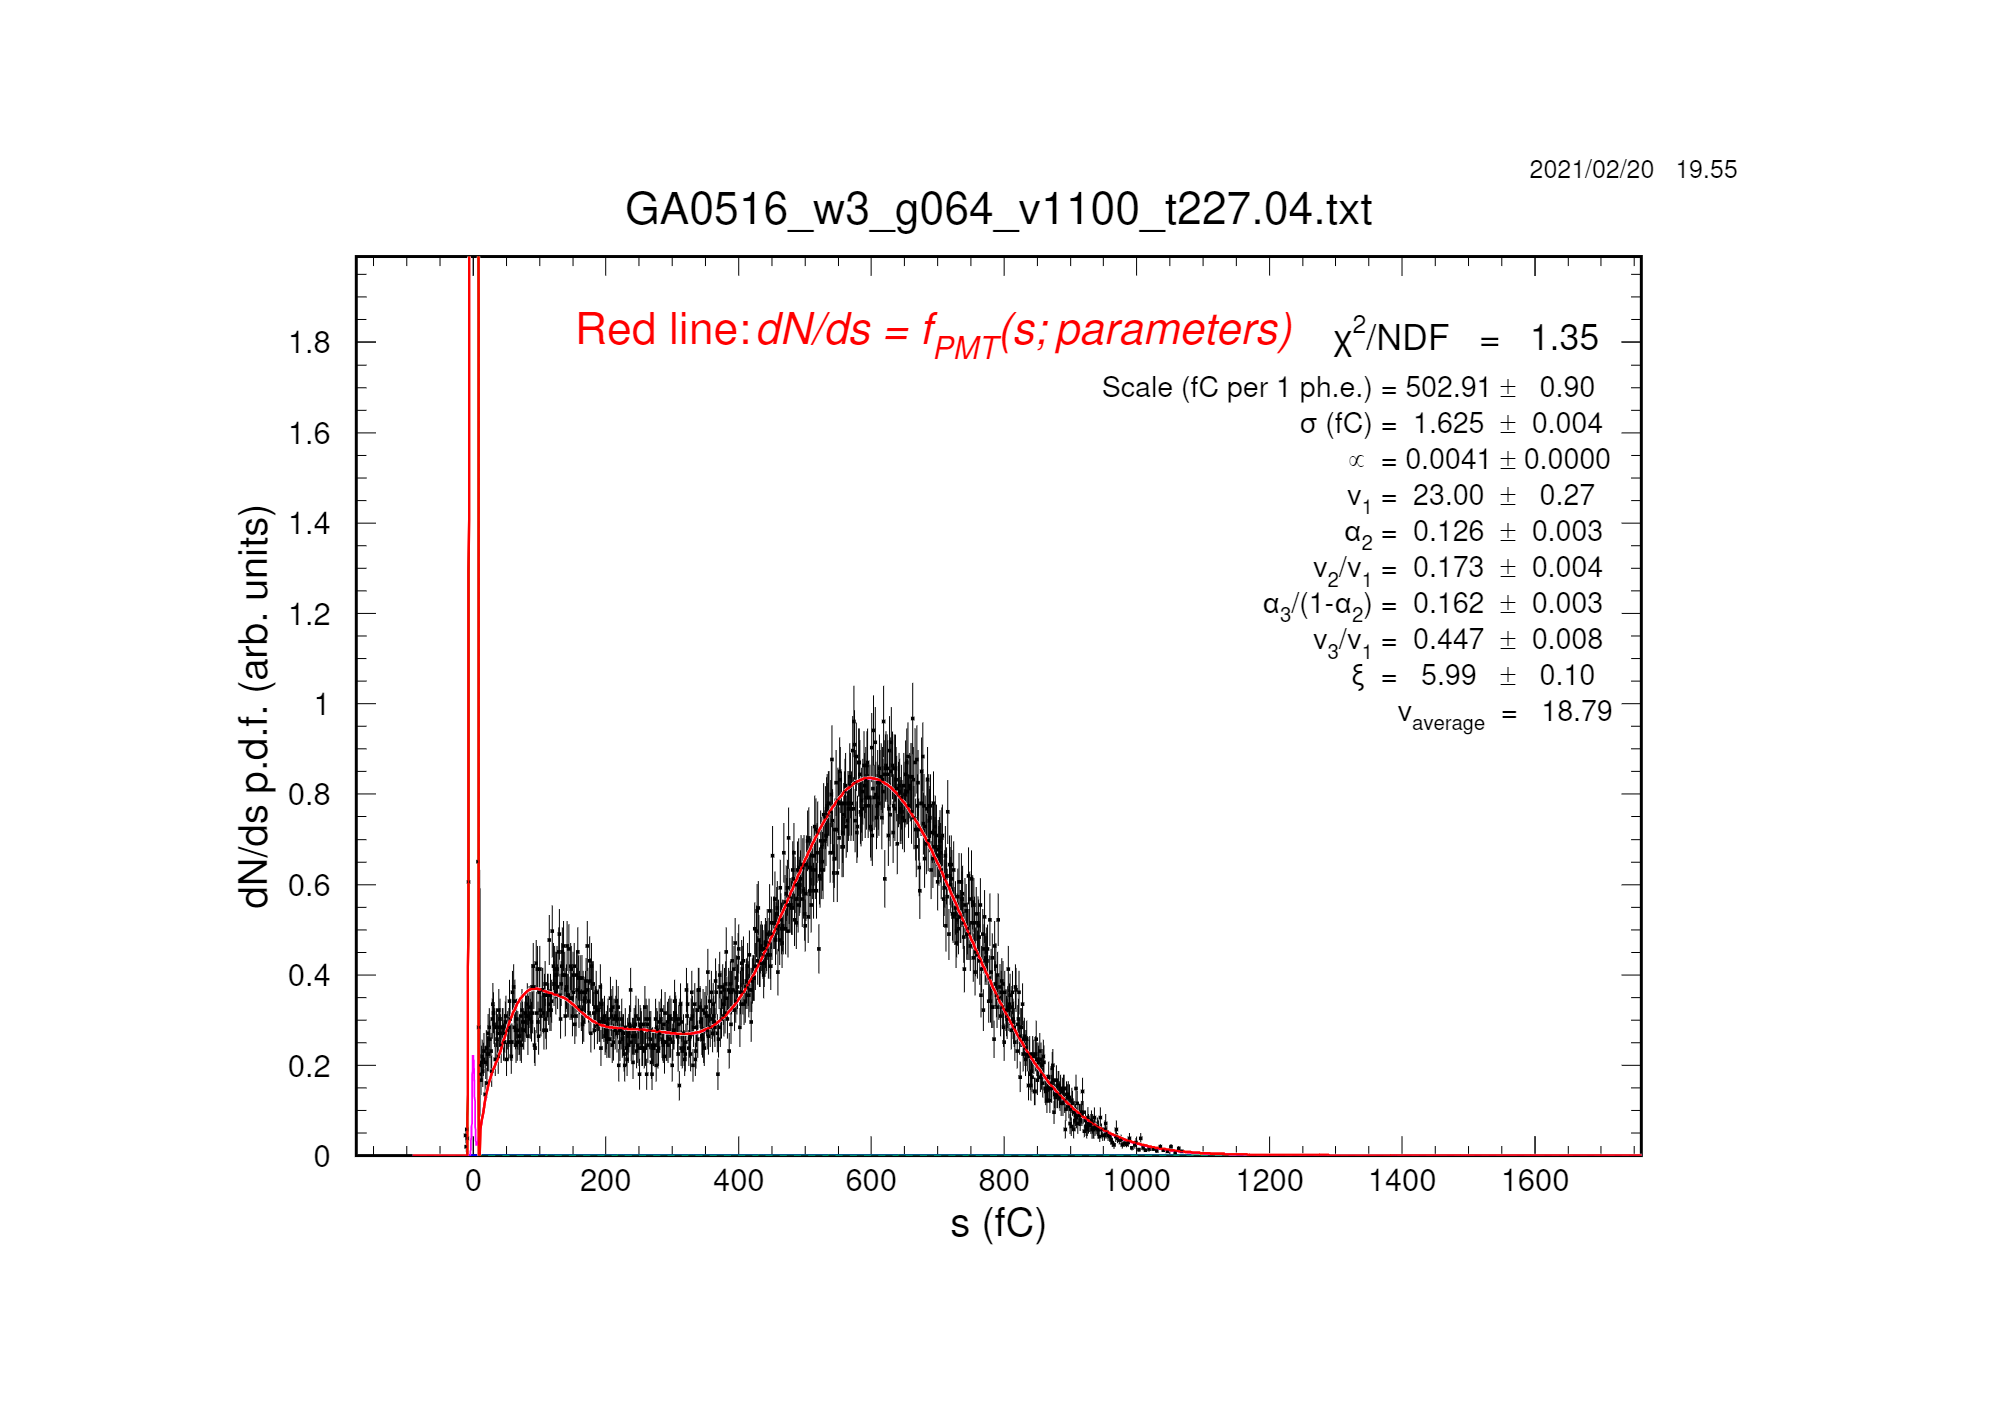
\includegraphics[width=\linewidth, trim={75mm 6cm 6cm 85mm},clip]{figures/GA0516_w3_g064_v1100_cln.04.png}
		\vspace{0mm}
	\end{subfigure}%%
	\vspace{0mm}
	\begin{subfigure}[c]{0.42\linewidth}
		\centering
		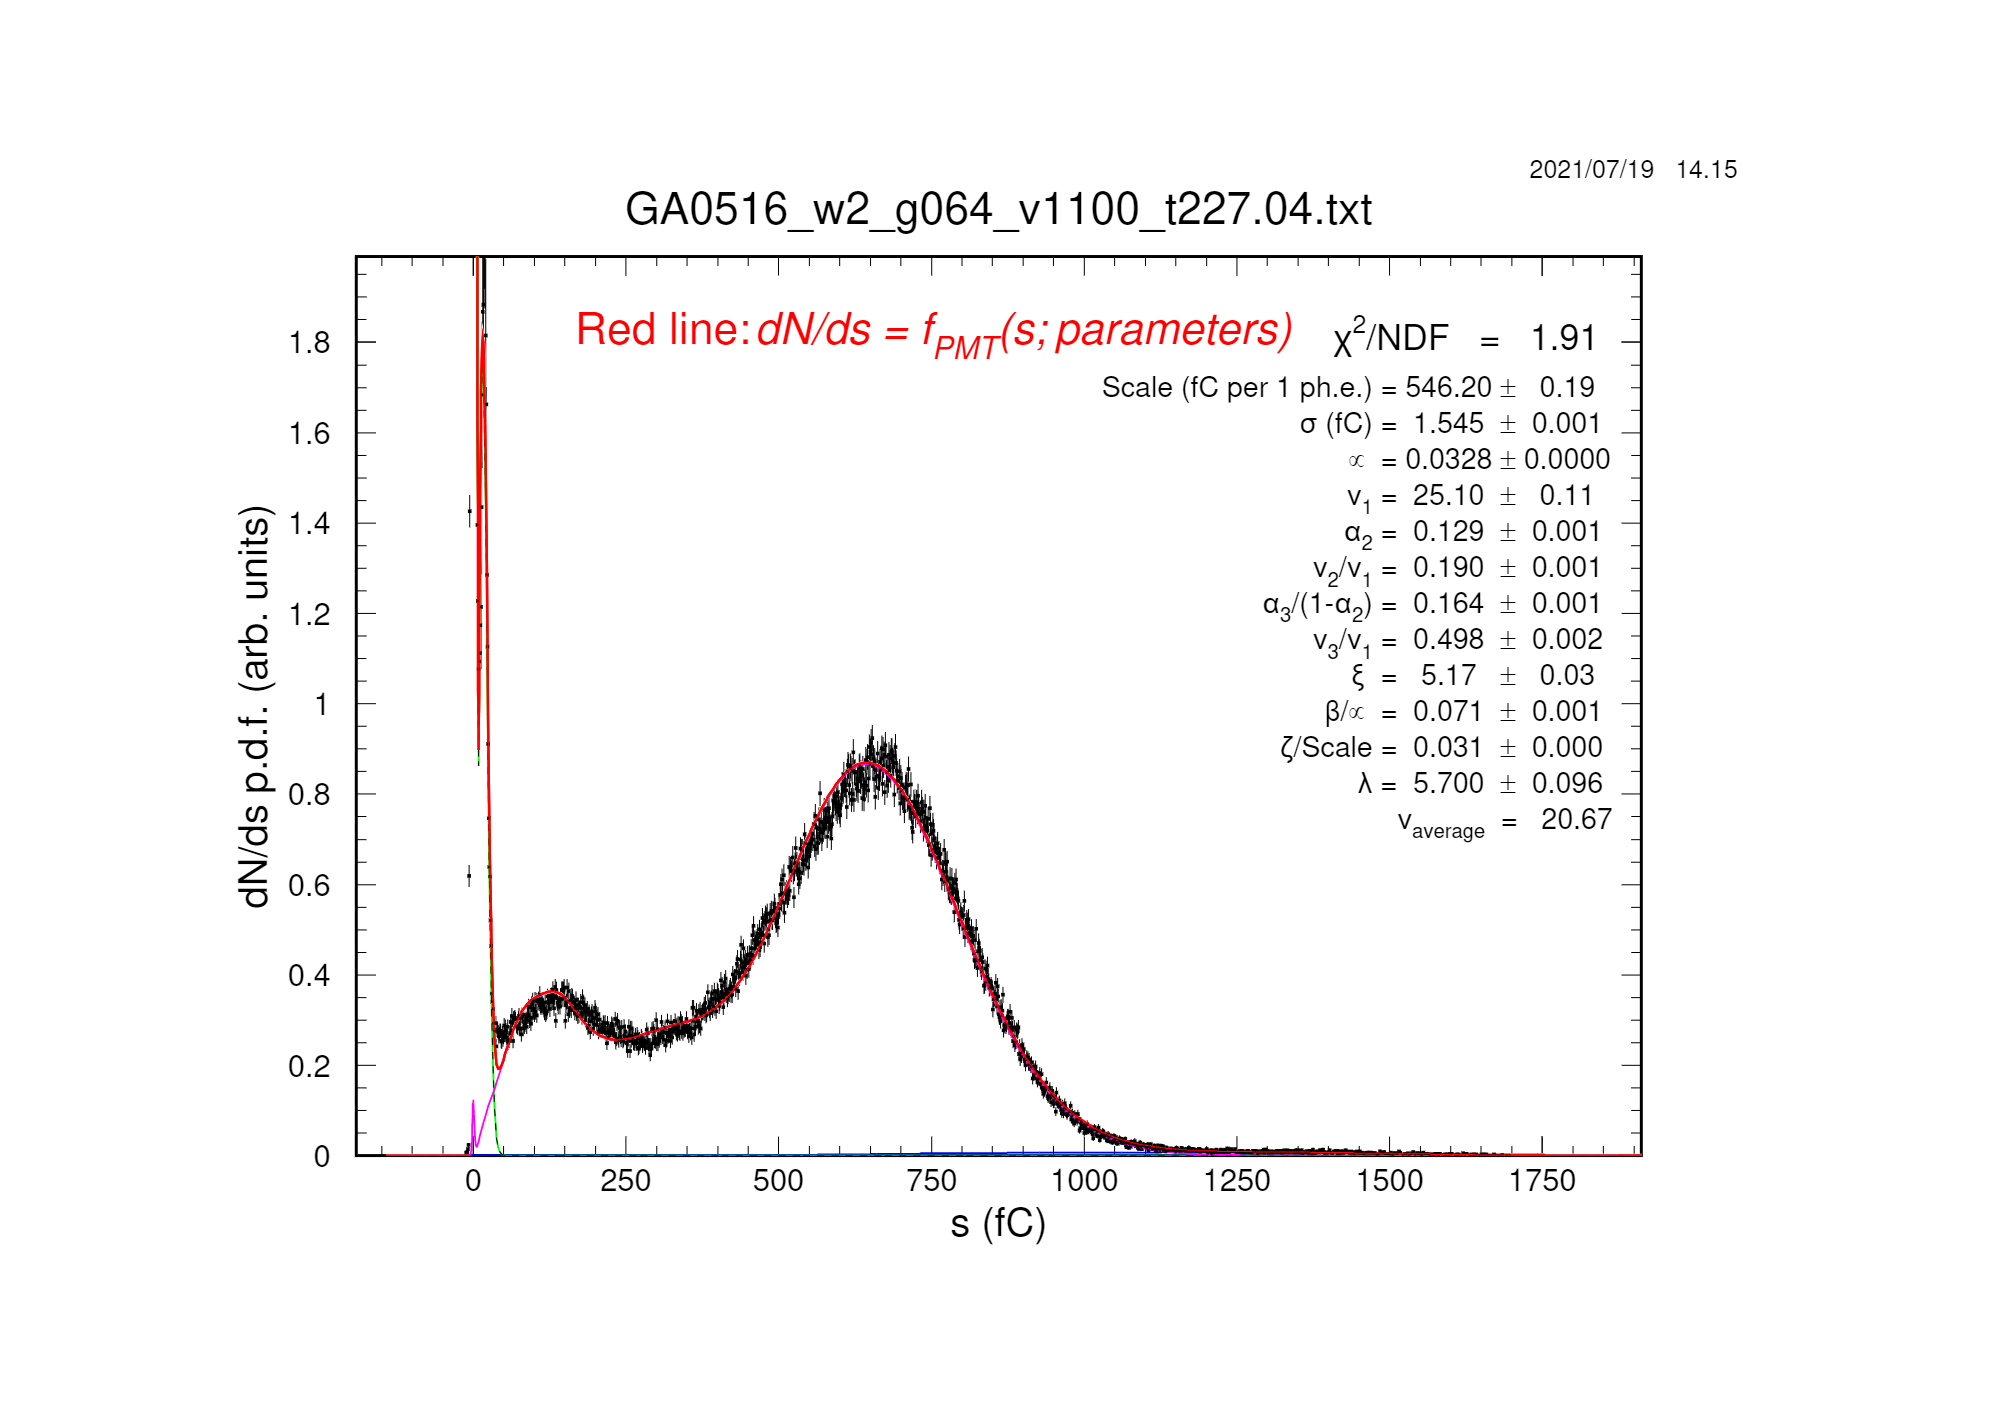
\includegraphics[width=\linewidth, trim={6cm 6cm 75mm 85mm},clip]{figures/GA0516_w2_g064_v1100_6mm.04.png}
		\vspace{0mm}
	\end{subfigure}%%
	\begin{subfigure}[c]{0.42\linewidth}
		\centering
		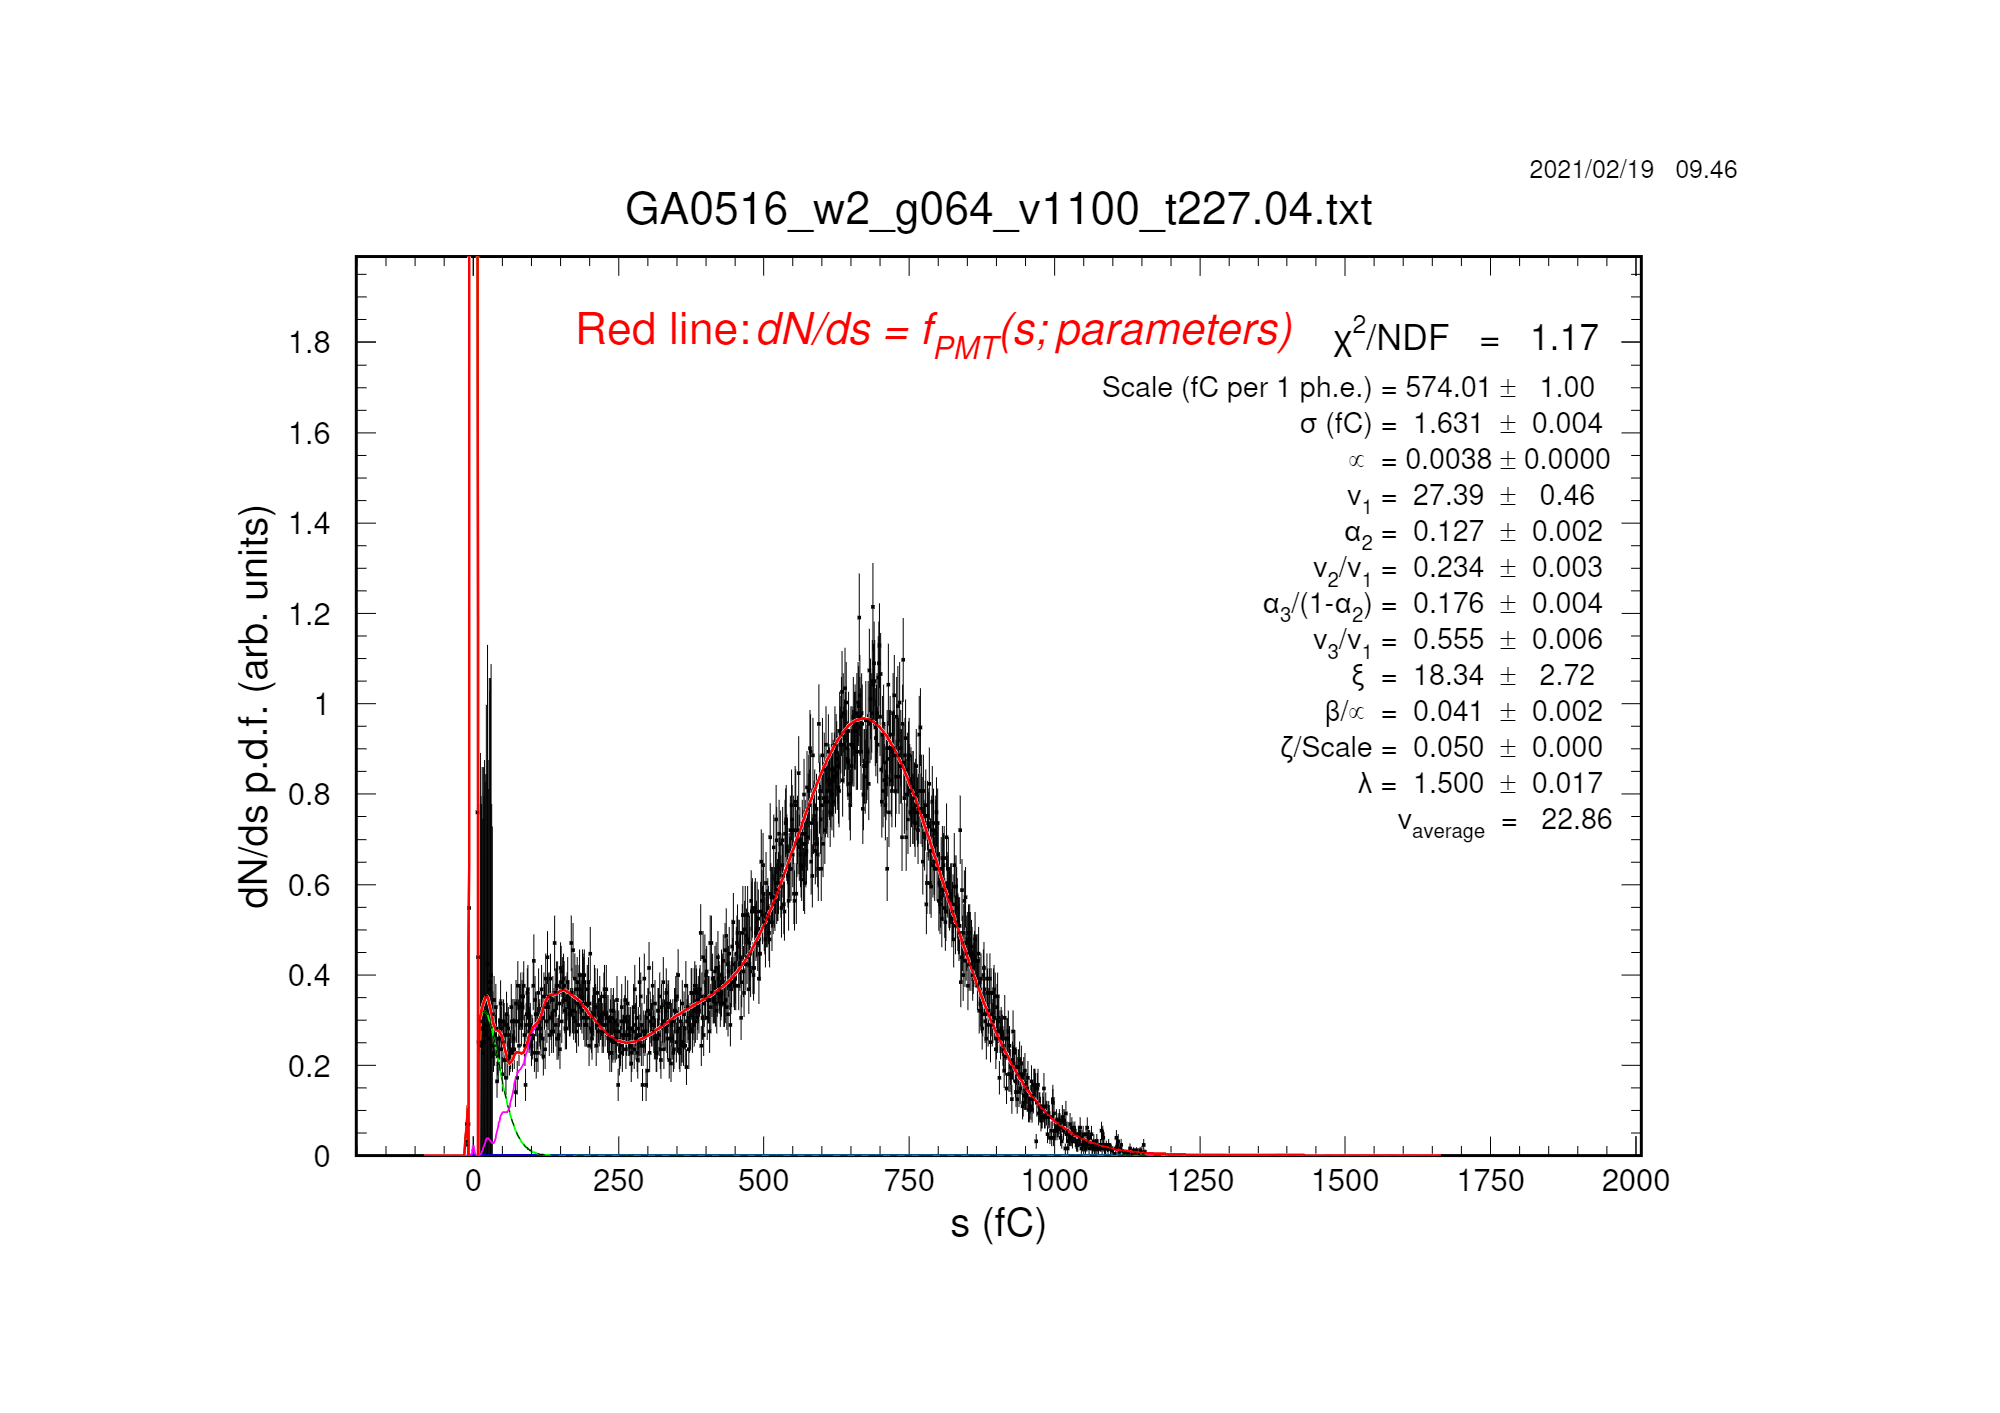
\includegraphics[width=\linewidth, trim={75mm 6cm 6cm 85mm},clip]{figures/GA0516_w3_g064_v1100_raw.04.png}
		\vspace{0mm}
	\end{subfigure}%%
	\caption{Same as Fig.~\ref{fig:GA0516_fits}, but all the data taken at HV = 1100 V.}
	\label{fig:GA0516_hv1100_fits}
\end{figure*}

\begin{figure*}[b]
	\centering
	\begin{subfigure}[c]{0.42\linewidth}
		\centering
		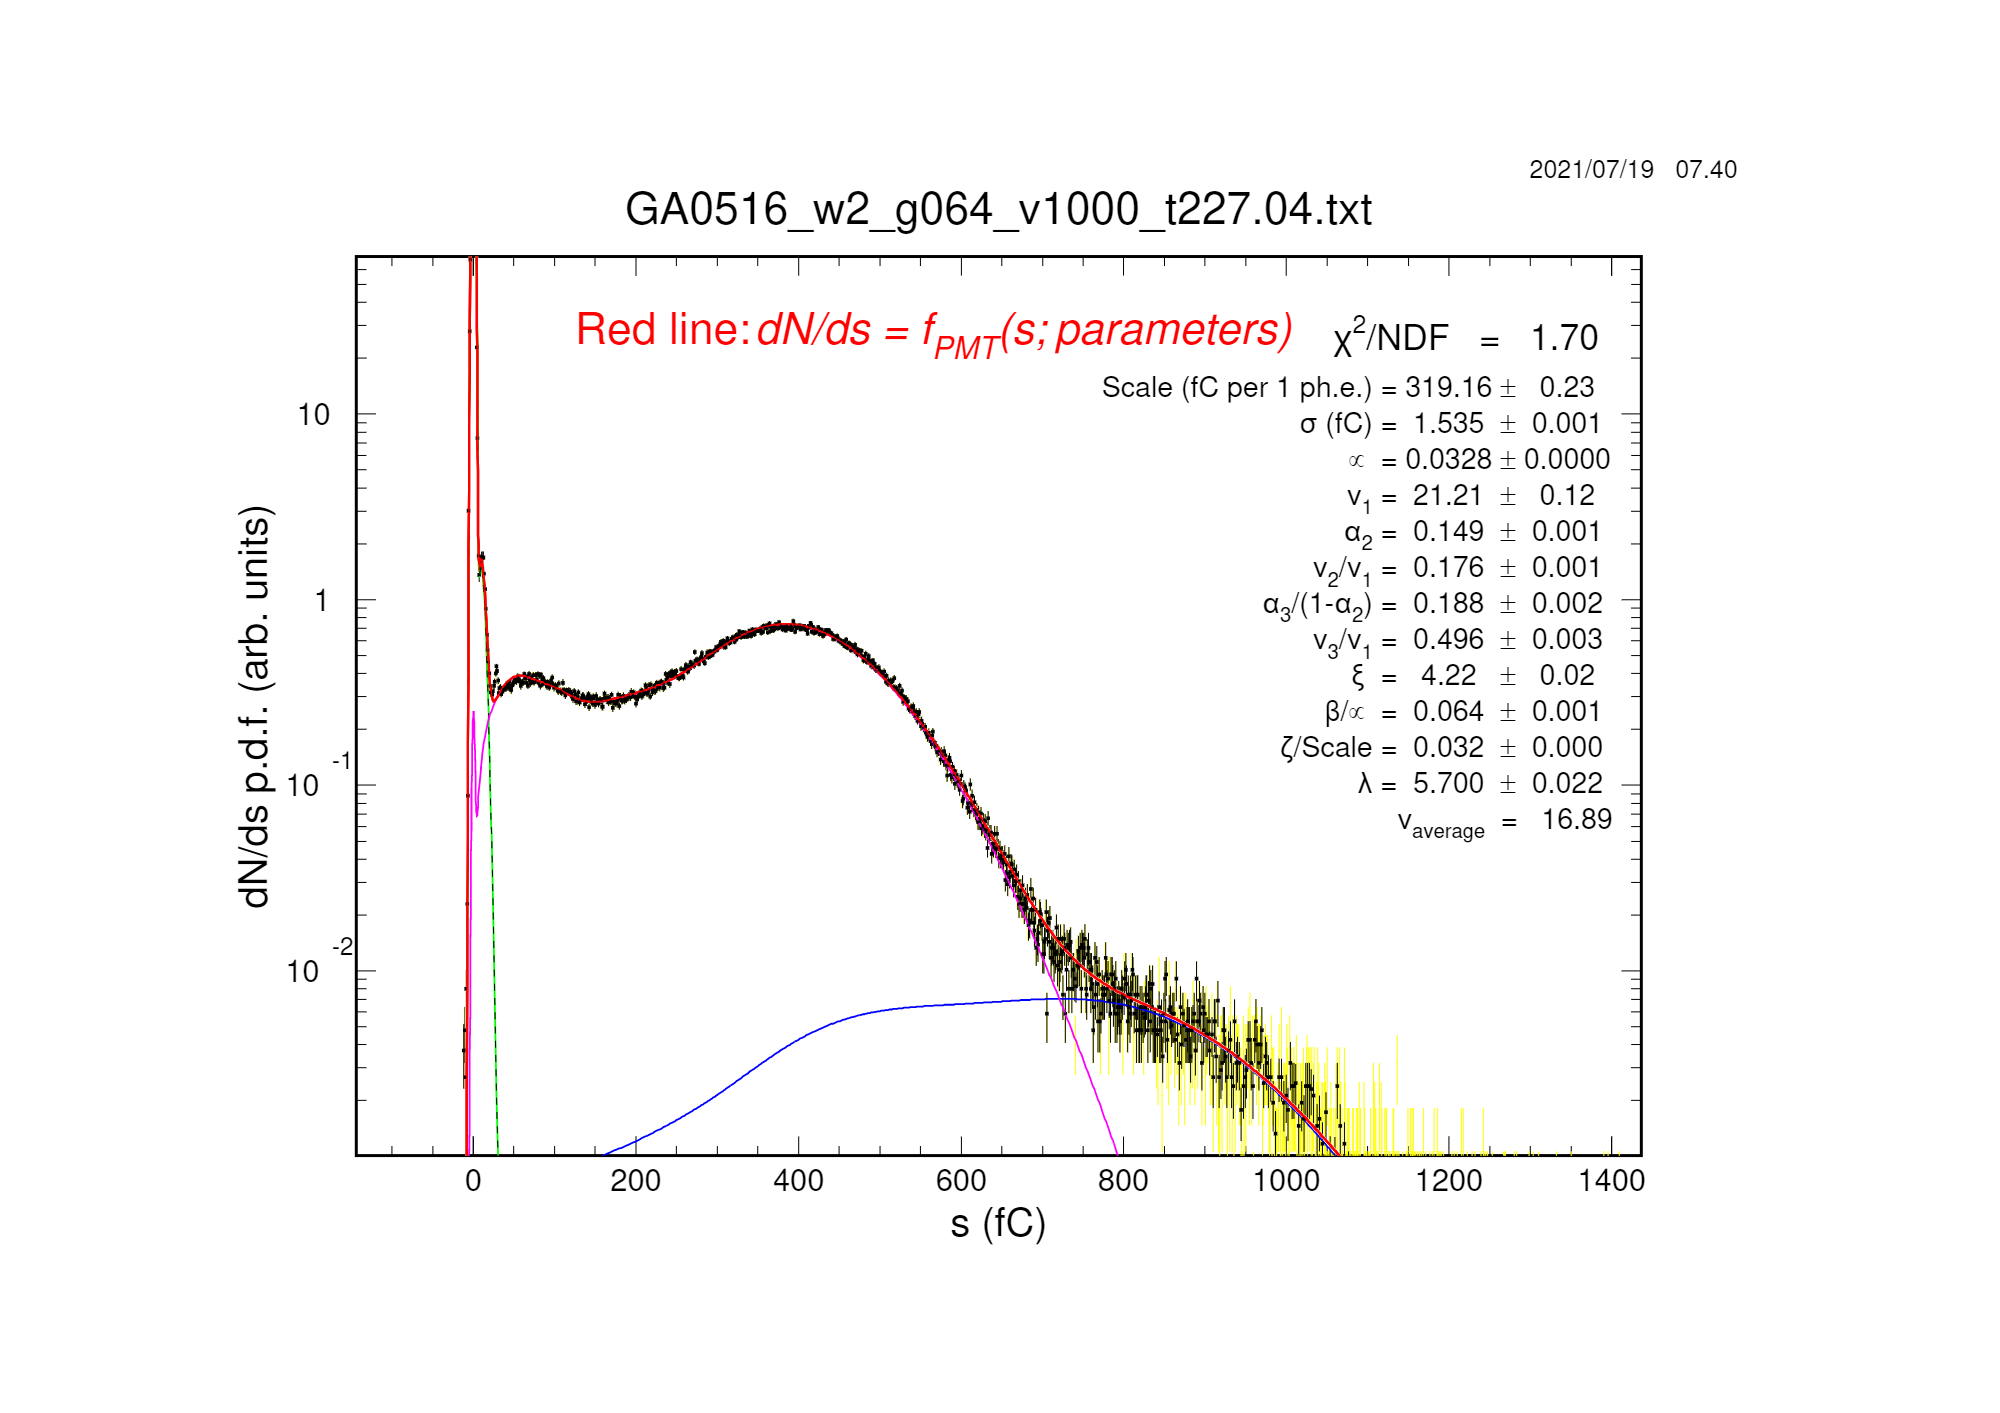
\includegraphics[width=\linewidth, trim={6cm 6cm 75mm 85mm},clip]{figures/GA0516_w2_g064_v1000_6mm_log.04.png}
		\vspace{0mm}
	\end{subfigure}%%
	\begin{subfigure}[c]{0.42\linewidth}
		\centering
		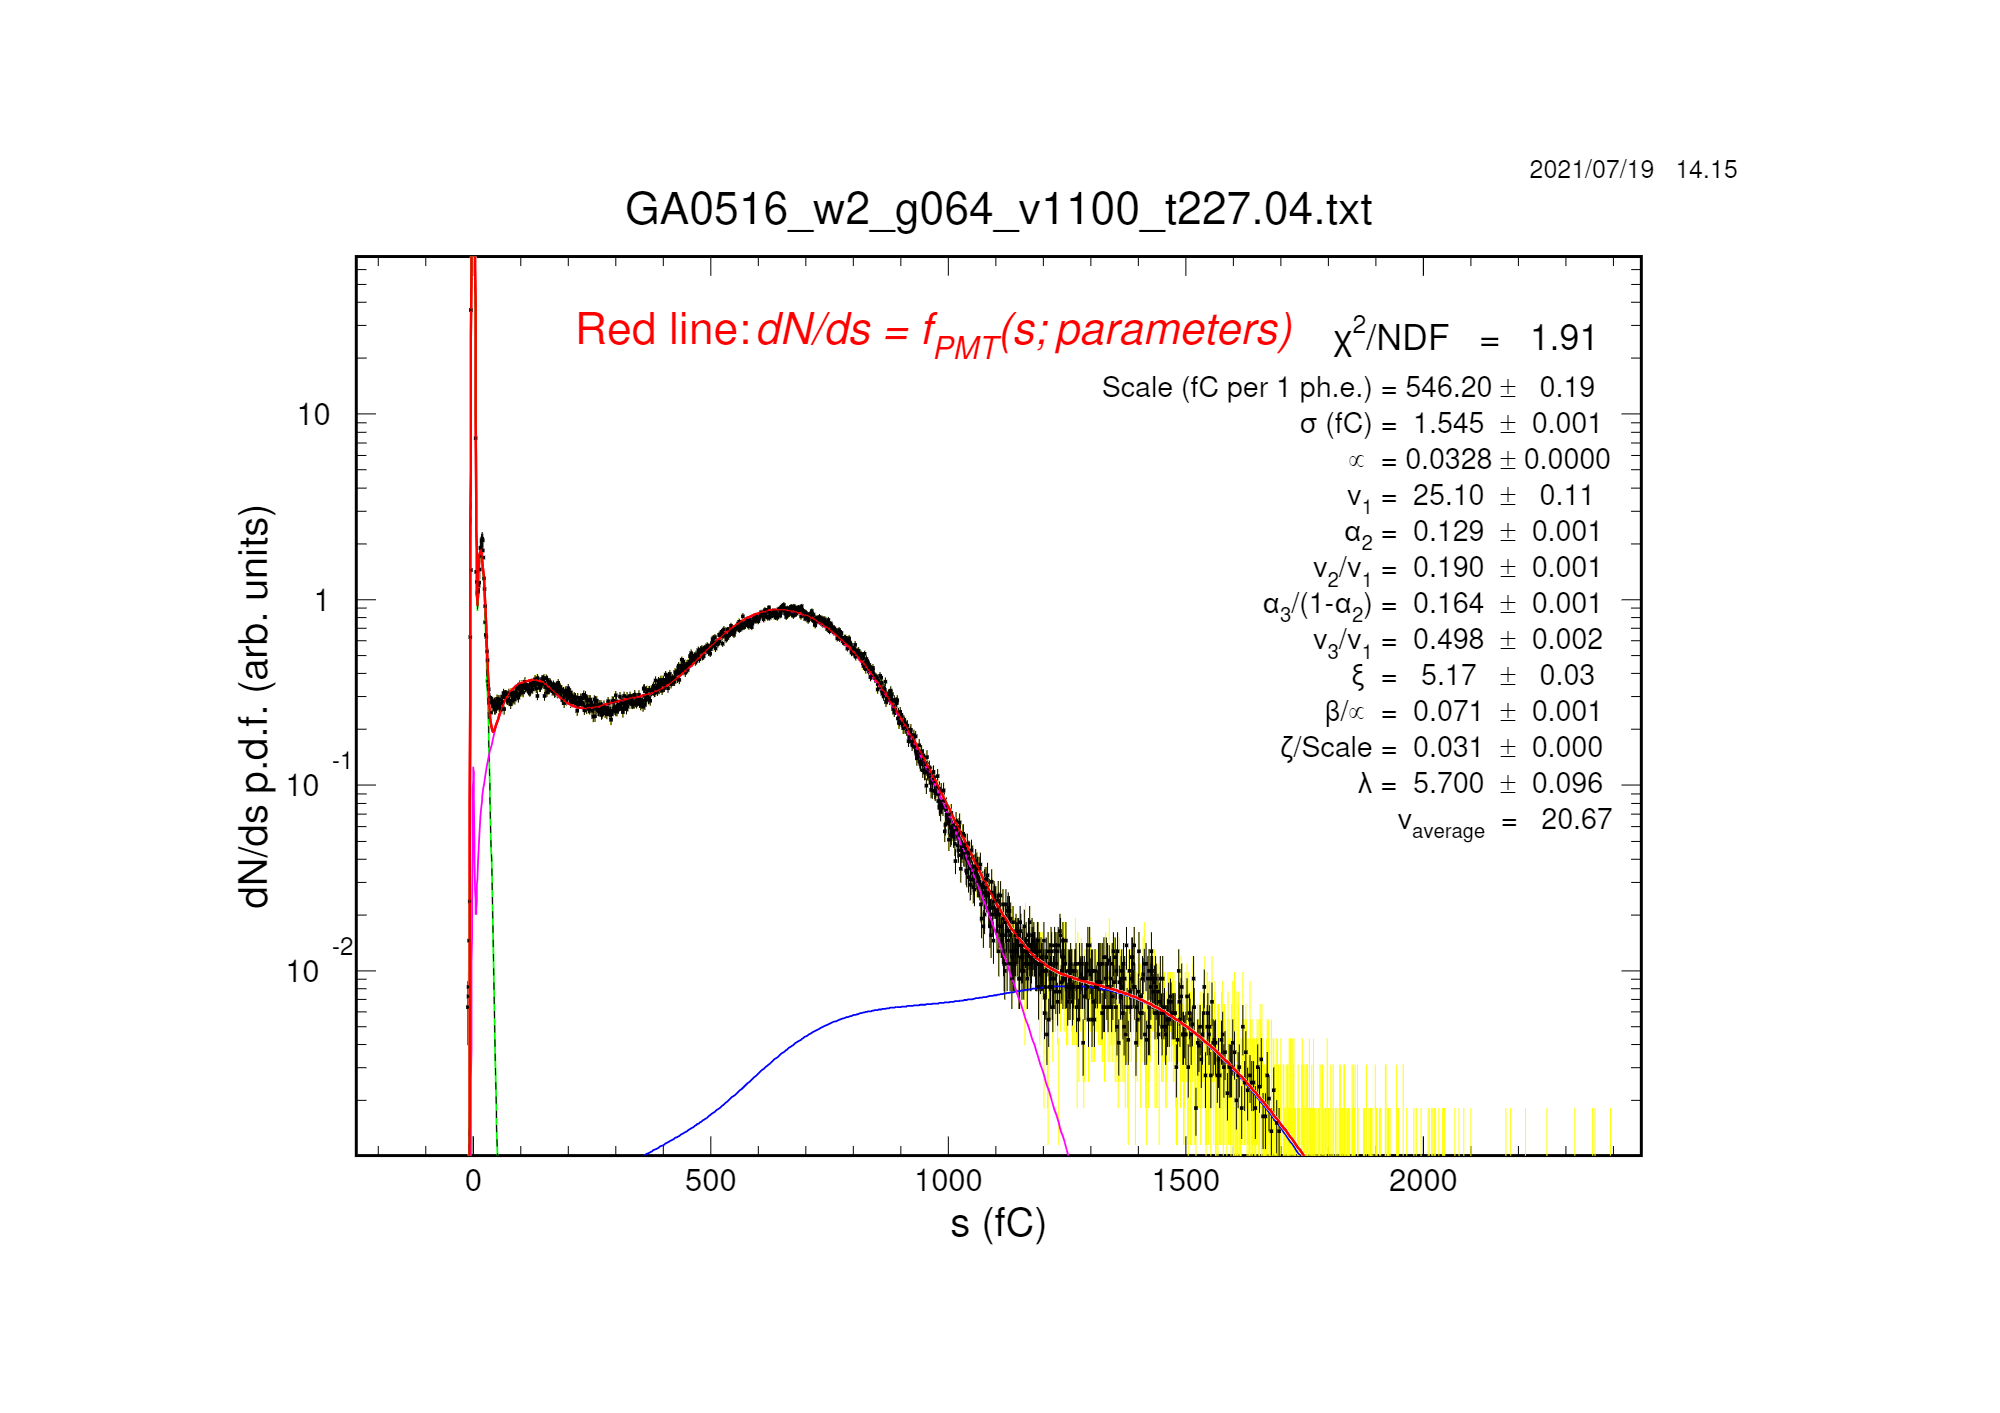
\includegraphics[width=\linewidth, trim={75mm 6cm 6cm 85mm},clip]{figures/GA0516_w2_g064_v1100_6mm_log.04.png}
		\vspace{0mm}
	\end{subfigure}%%
	\vspace{0mm}
	\begin{subfigure}[c]{0.42\linewidth}
		\centering
		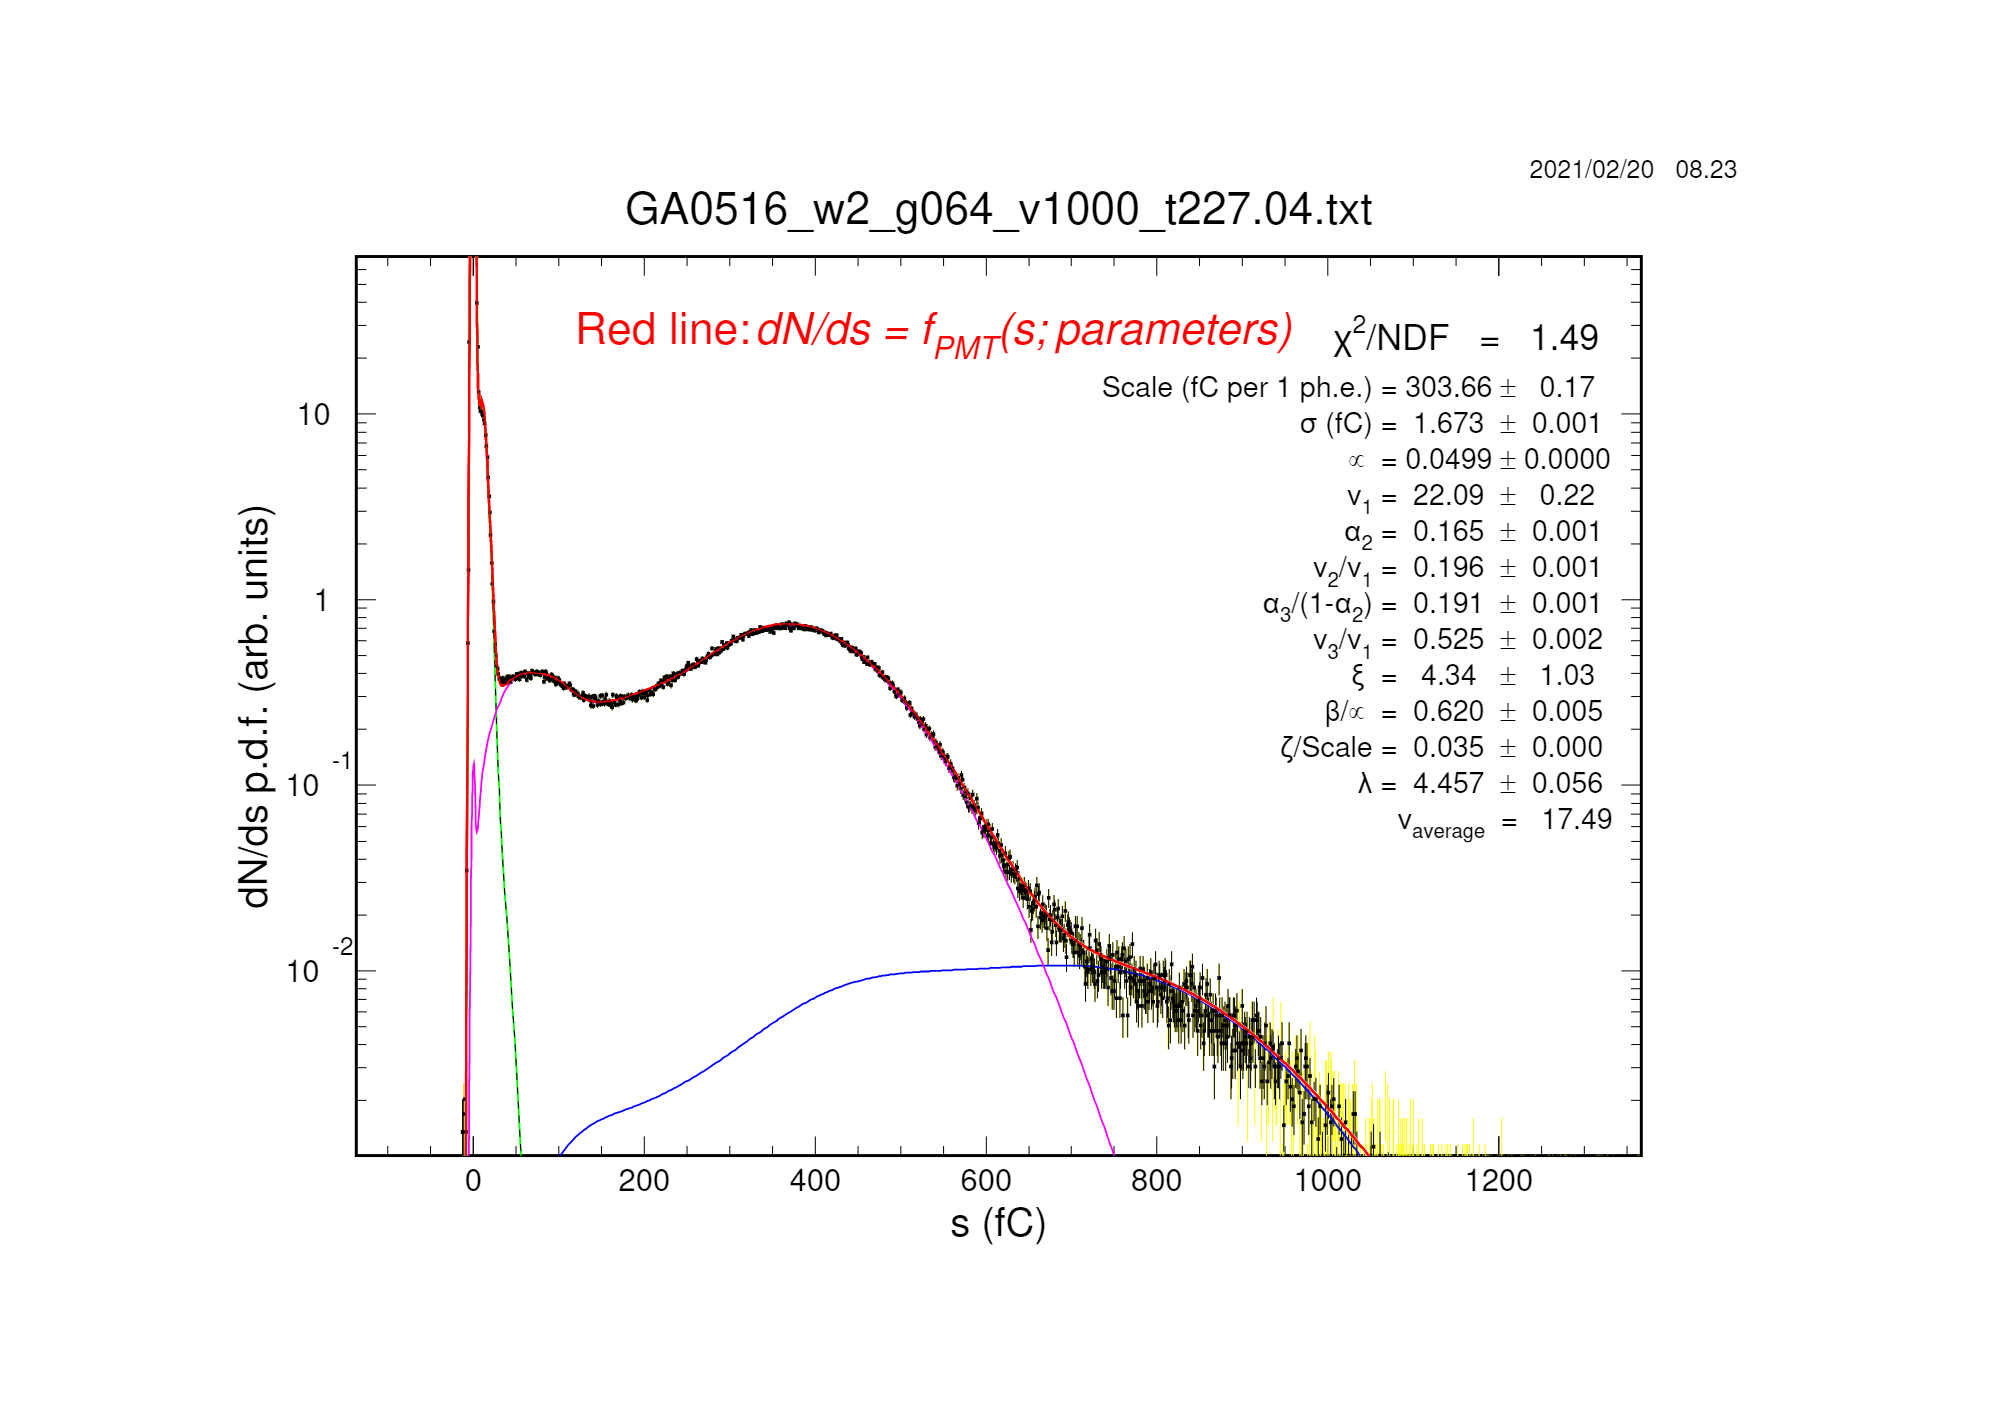
\includegraphics[width=\linewidth, trim={6cm 6cm 75mm 85mm},clip]{figures/GA0516_w2_g064_v1000_raw_log.04.png}
		\vspace{0mm}
	\end{subfigure}%%
	\begin{subfigure}[c]{0.42\linewidth}
		\centering
		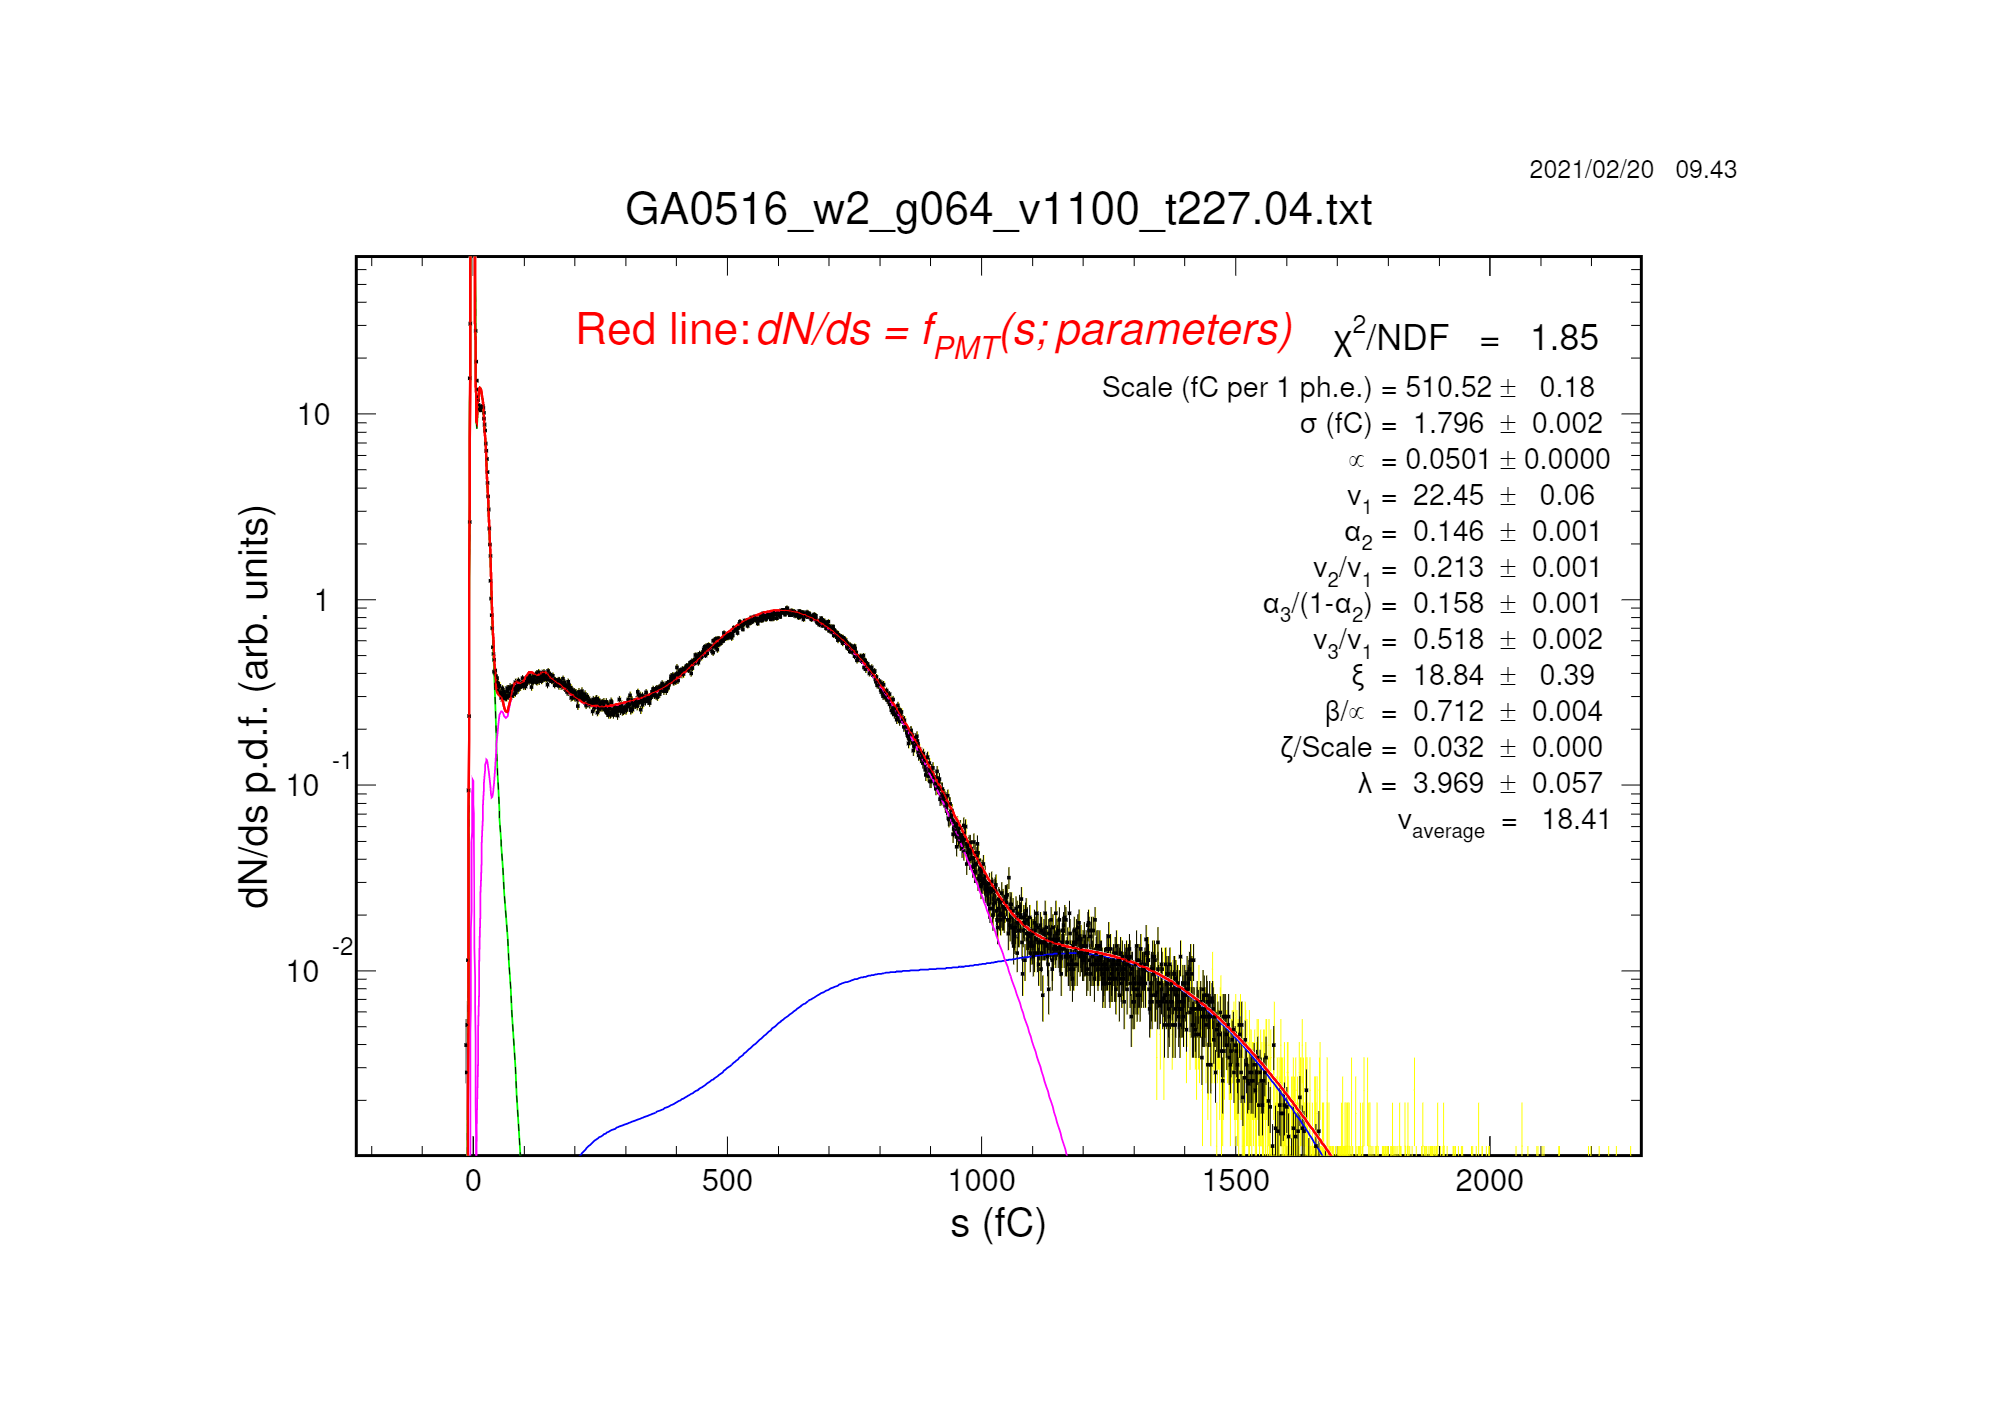
\includegraphics[width=\linewidth, trim={75mm 6cm 6cm 85mm},clip]{figures/GA0516_w2_g064_v1100_raw_log.04.png}
		\vspace{0mm}
	\end{subfigure}%%
	\caption{SPE probability distributions for PMT GA0516, pixel 4, wheel position 2, at HV = 1000 V (left plots) and at HV = 1100 V (right plots). Top plots: run with 6 mm mask covering the full PMT face except pixel 4. Bottom plots: run with full PMT face open, the contribution to the spectrum from the crosstalk events is approximated and parametrized by the analysis algorithm.}
	\label{fig:GA0516_w2_fits}
\end{figure*}

\begin{figure*}[b]
	\centering
	\begin{subfigure}[c]{0.42\linewidth}
		\centering
		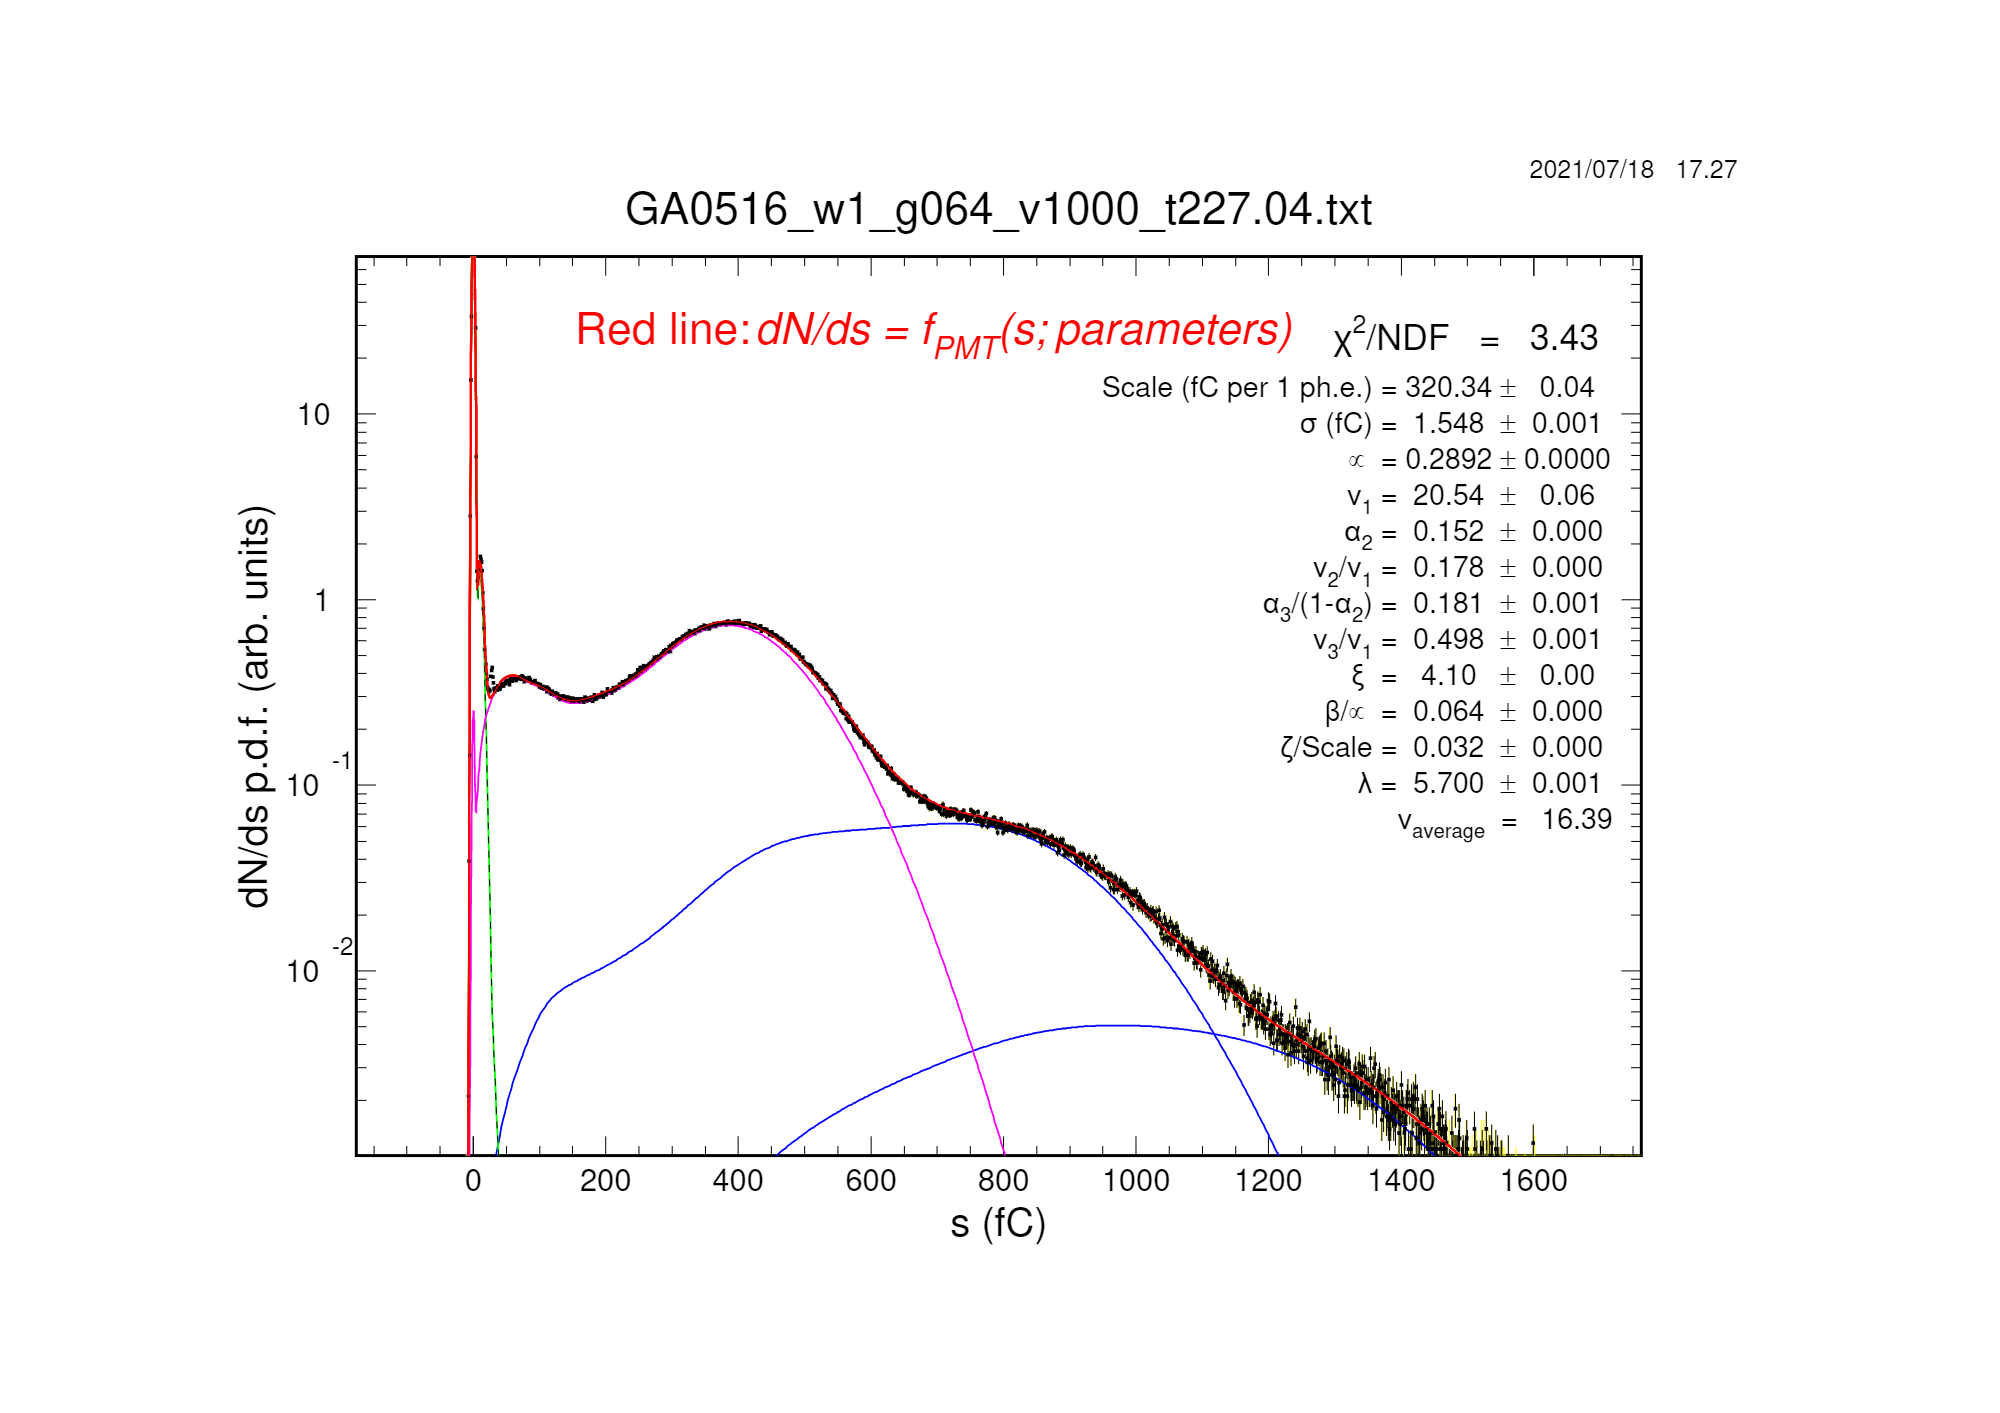
\includegraphics[width=\linewidth, trim={6cm 6cm 75mm 85mm},clip]{figures/GA0516_w1_g064_v1000_6mm_log.04.png}
		\vspace{0mm}
	\end{subfigure}%%
	\begin{subfigure}[c]{0.42\linewidth}
		\centering
		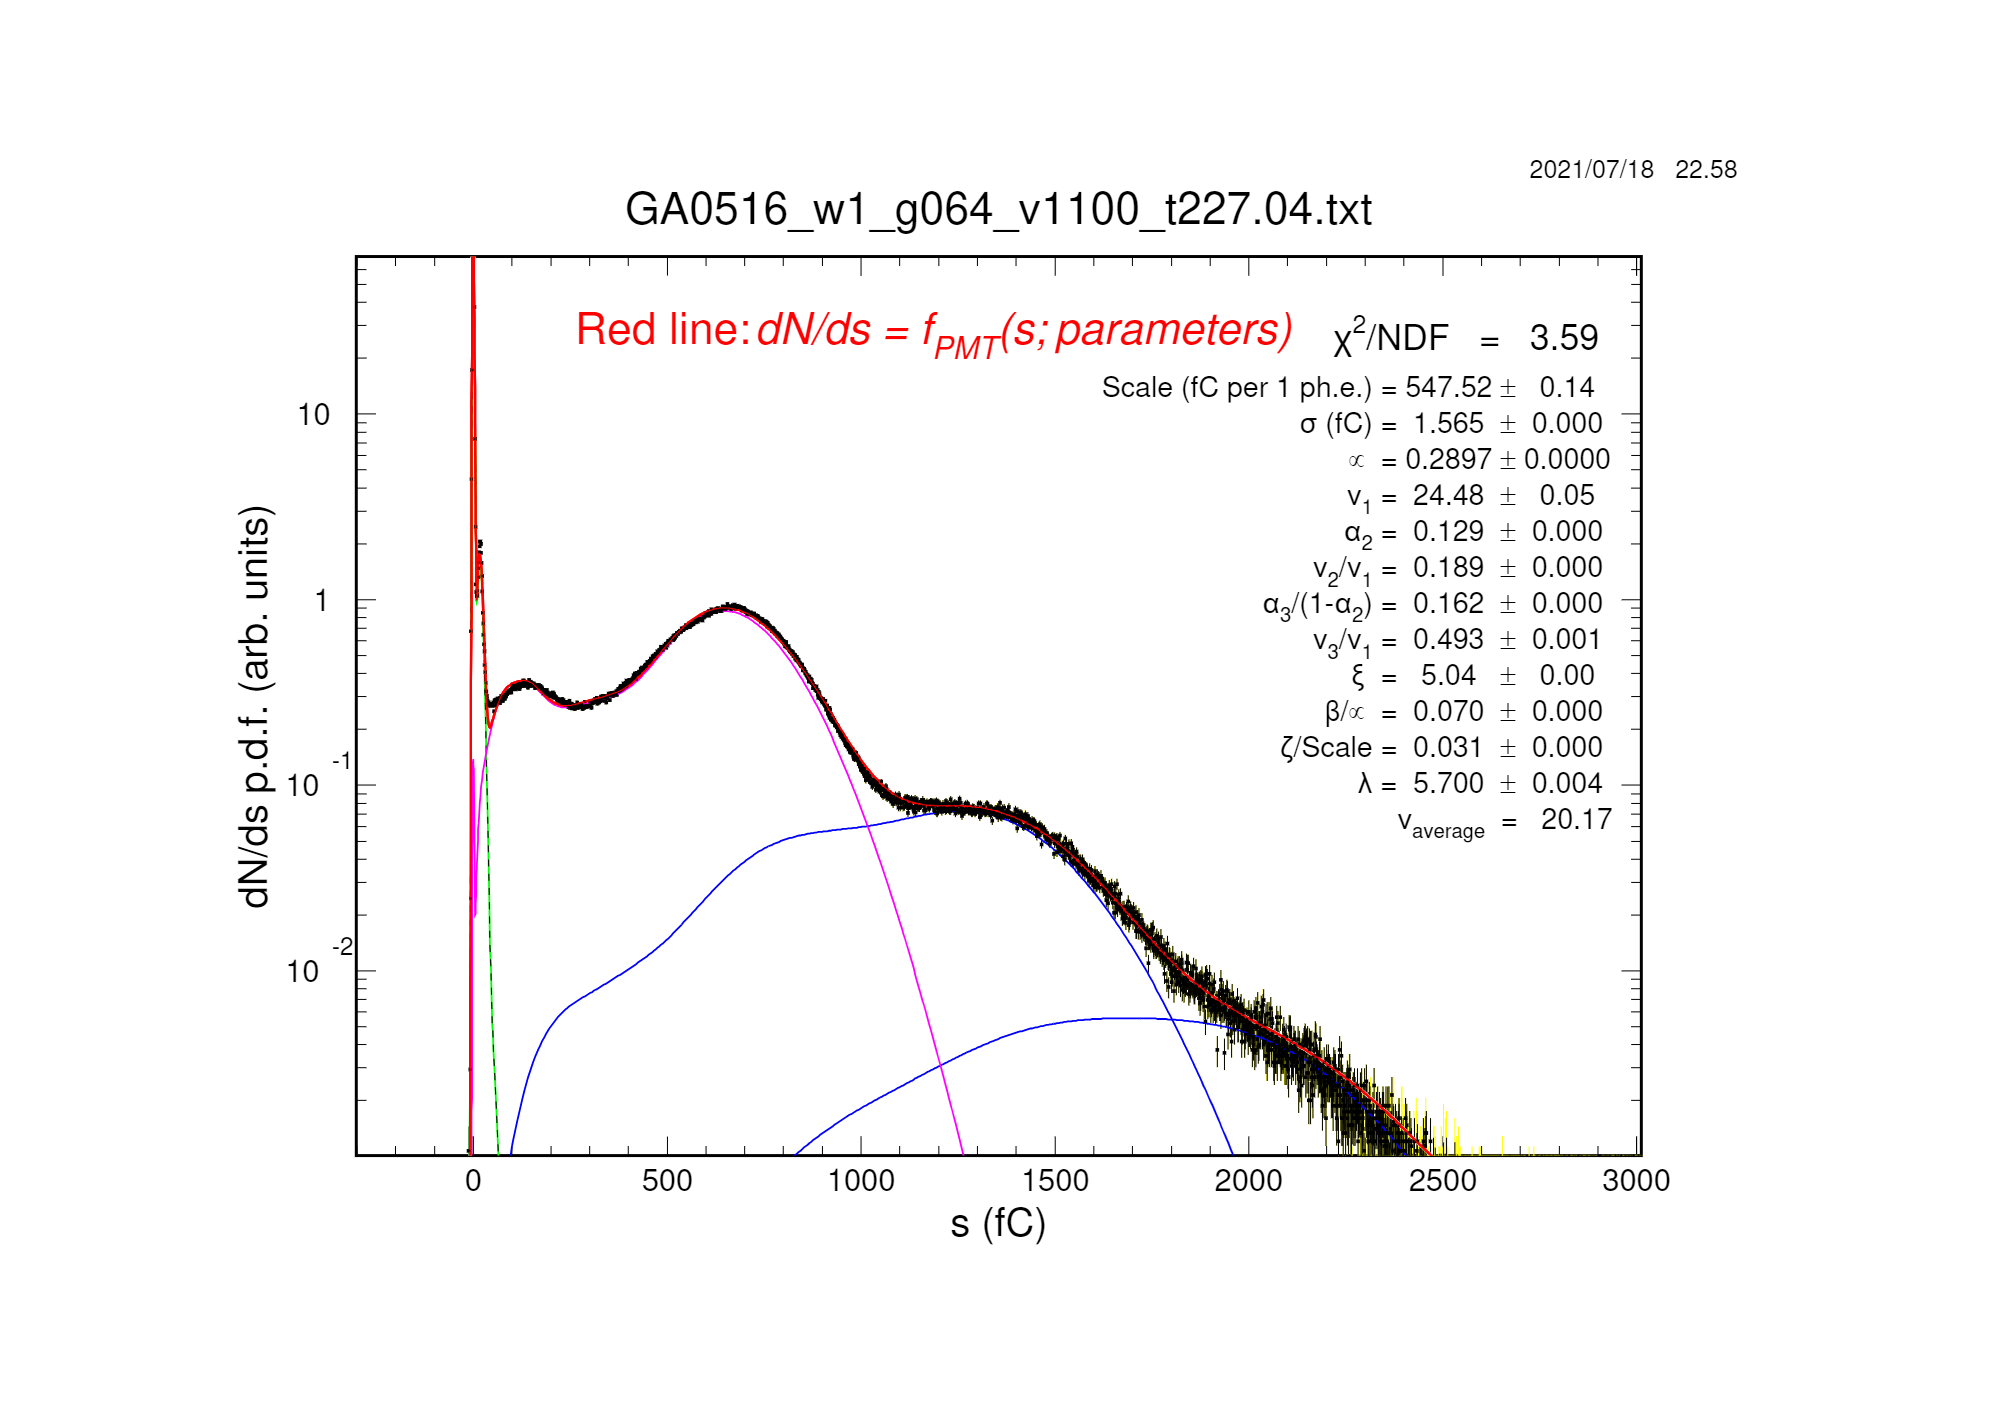
\includegraphics[width=\linewidth, trim={75mm 6cm 6cm 85mm},clip]{figures/GA0516_w1_g064_v1100_6mm_log.04.png}
		\vspace{0mm}
	\end{subfigure}%%
	\vspace{0mm}
	\begin{subfigure}[c]{0.42\linewidth}
		\centering
		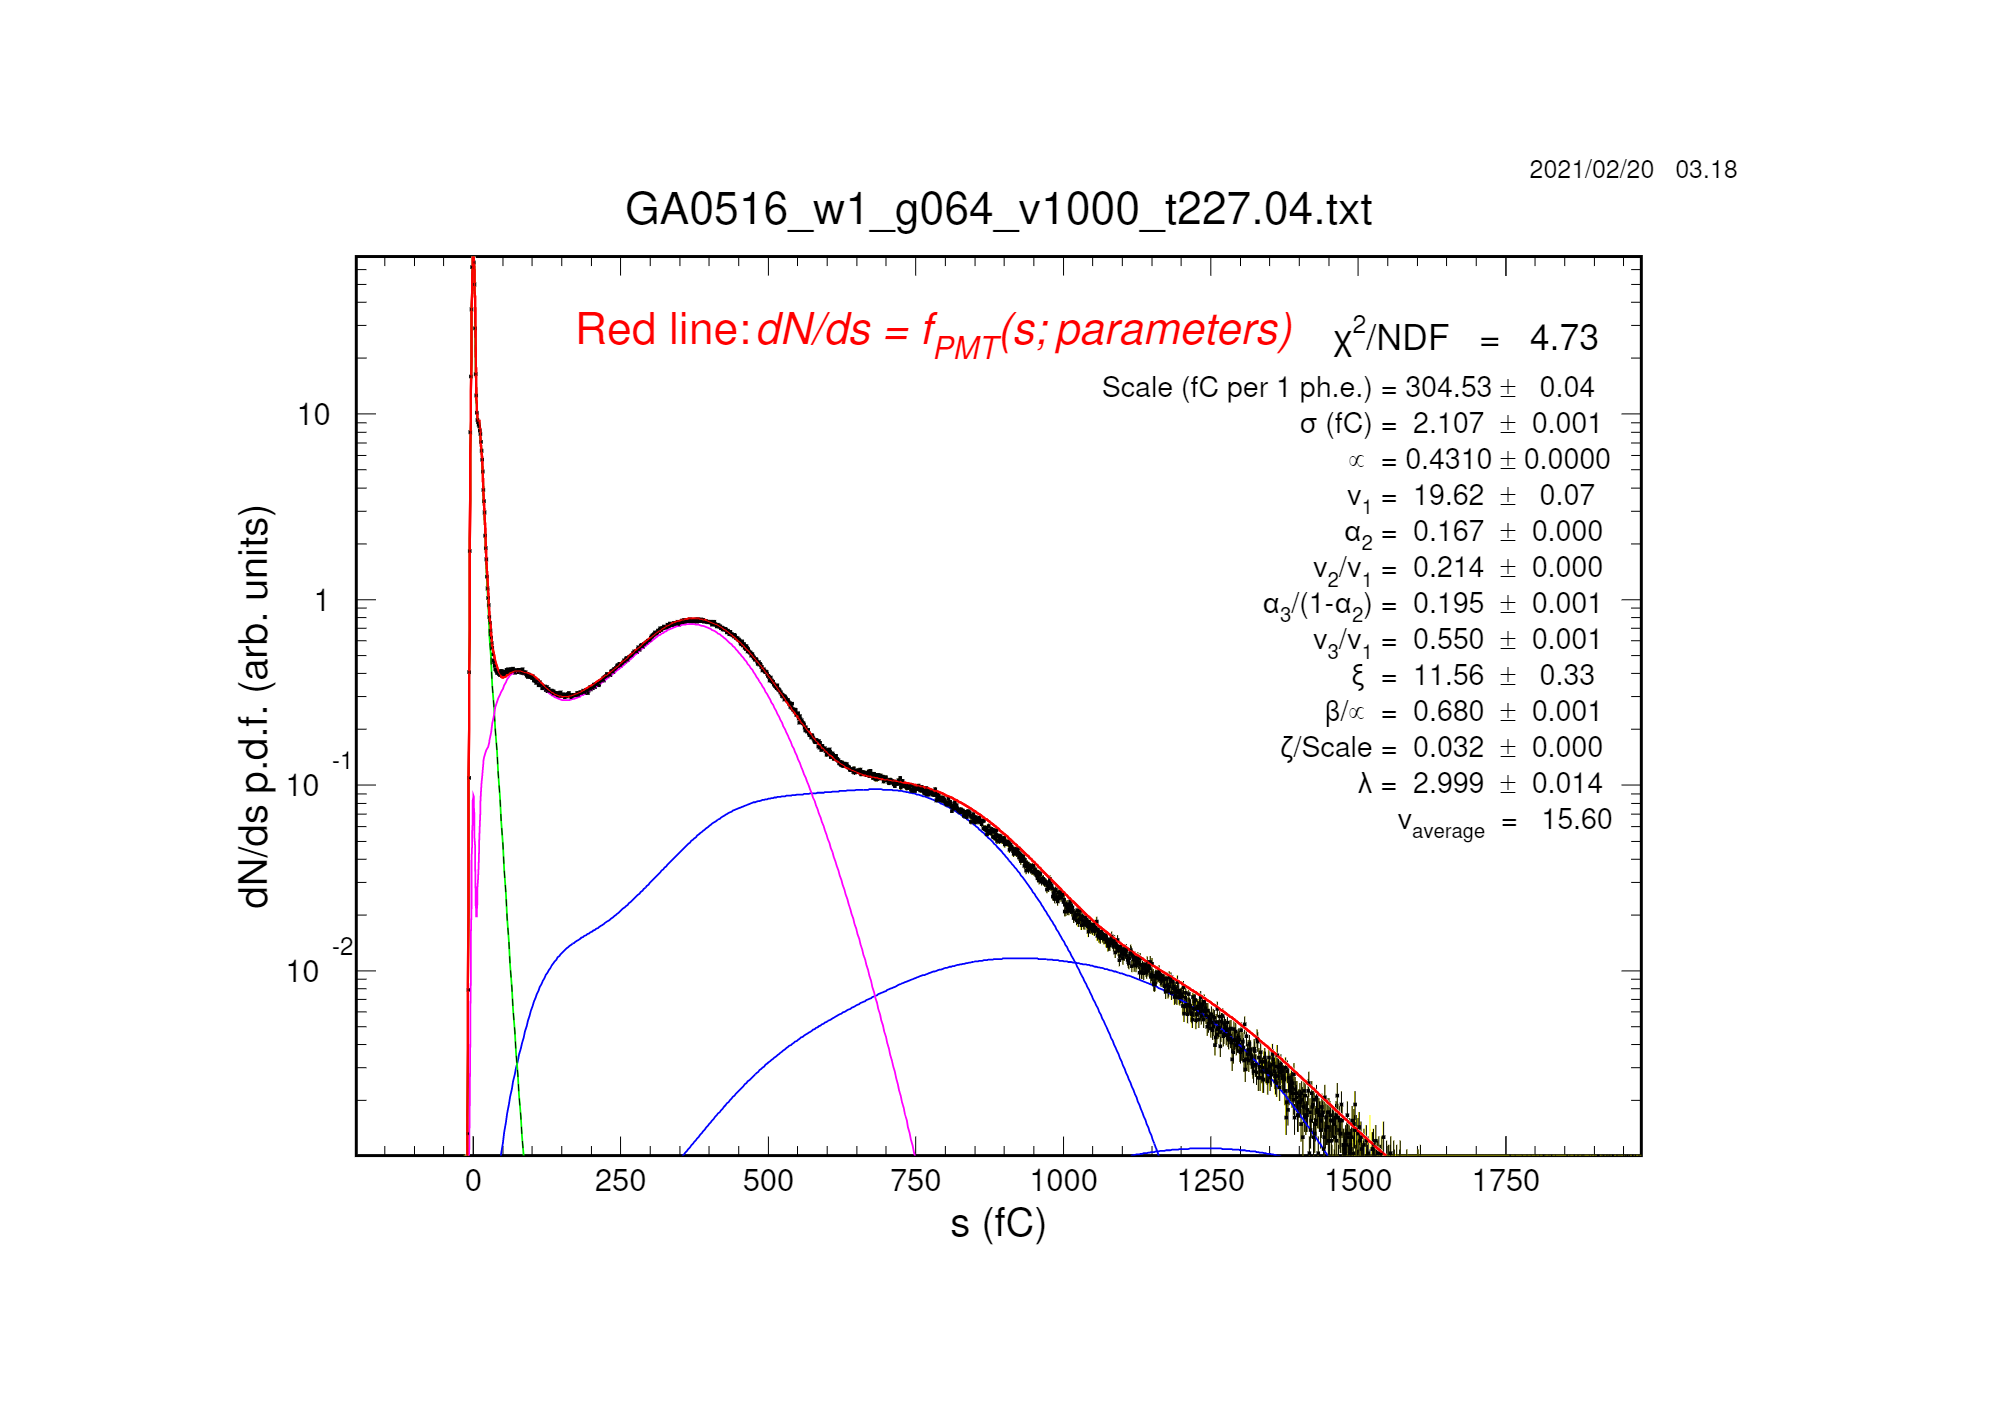
\includegraphics[width=\linewidth, trim={6cm 6cm 75mm 85mm},clip]{figures/GA0516_w1_g064_v1000_raw_log.04.png}
		\vspace{0mm}
	\end{subfigure}%%
	\begin{subfigure}[c]{0.42\linewidth}
		\centering
		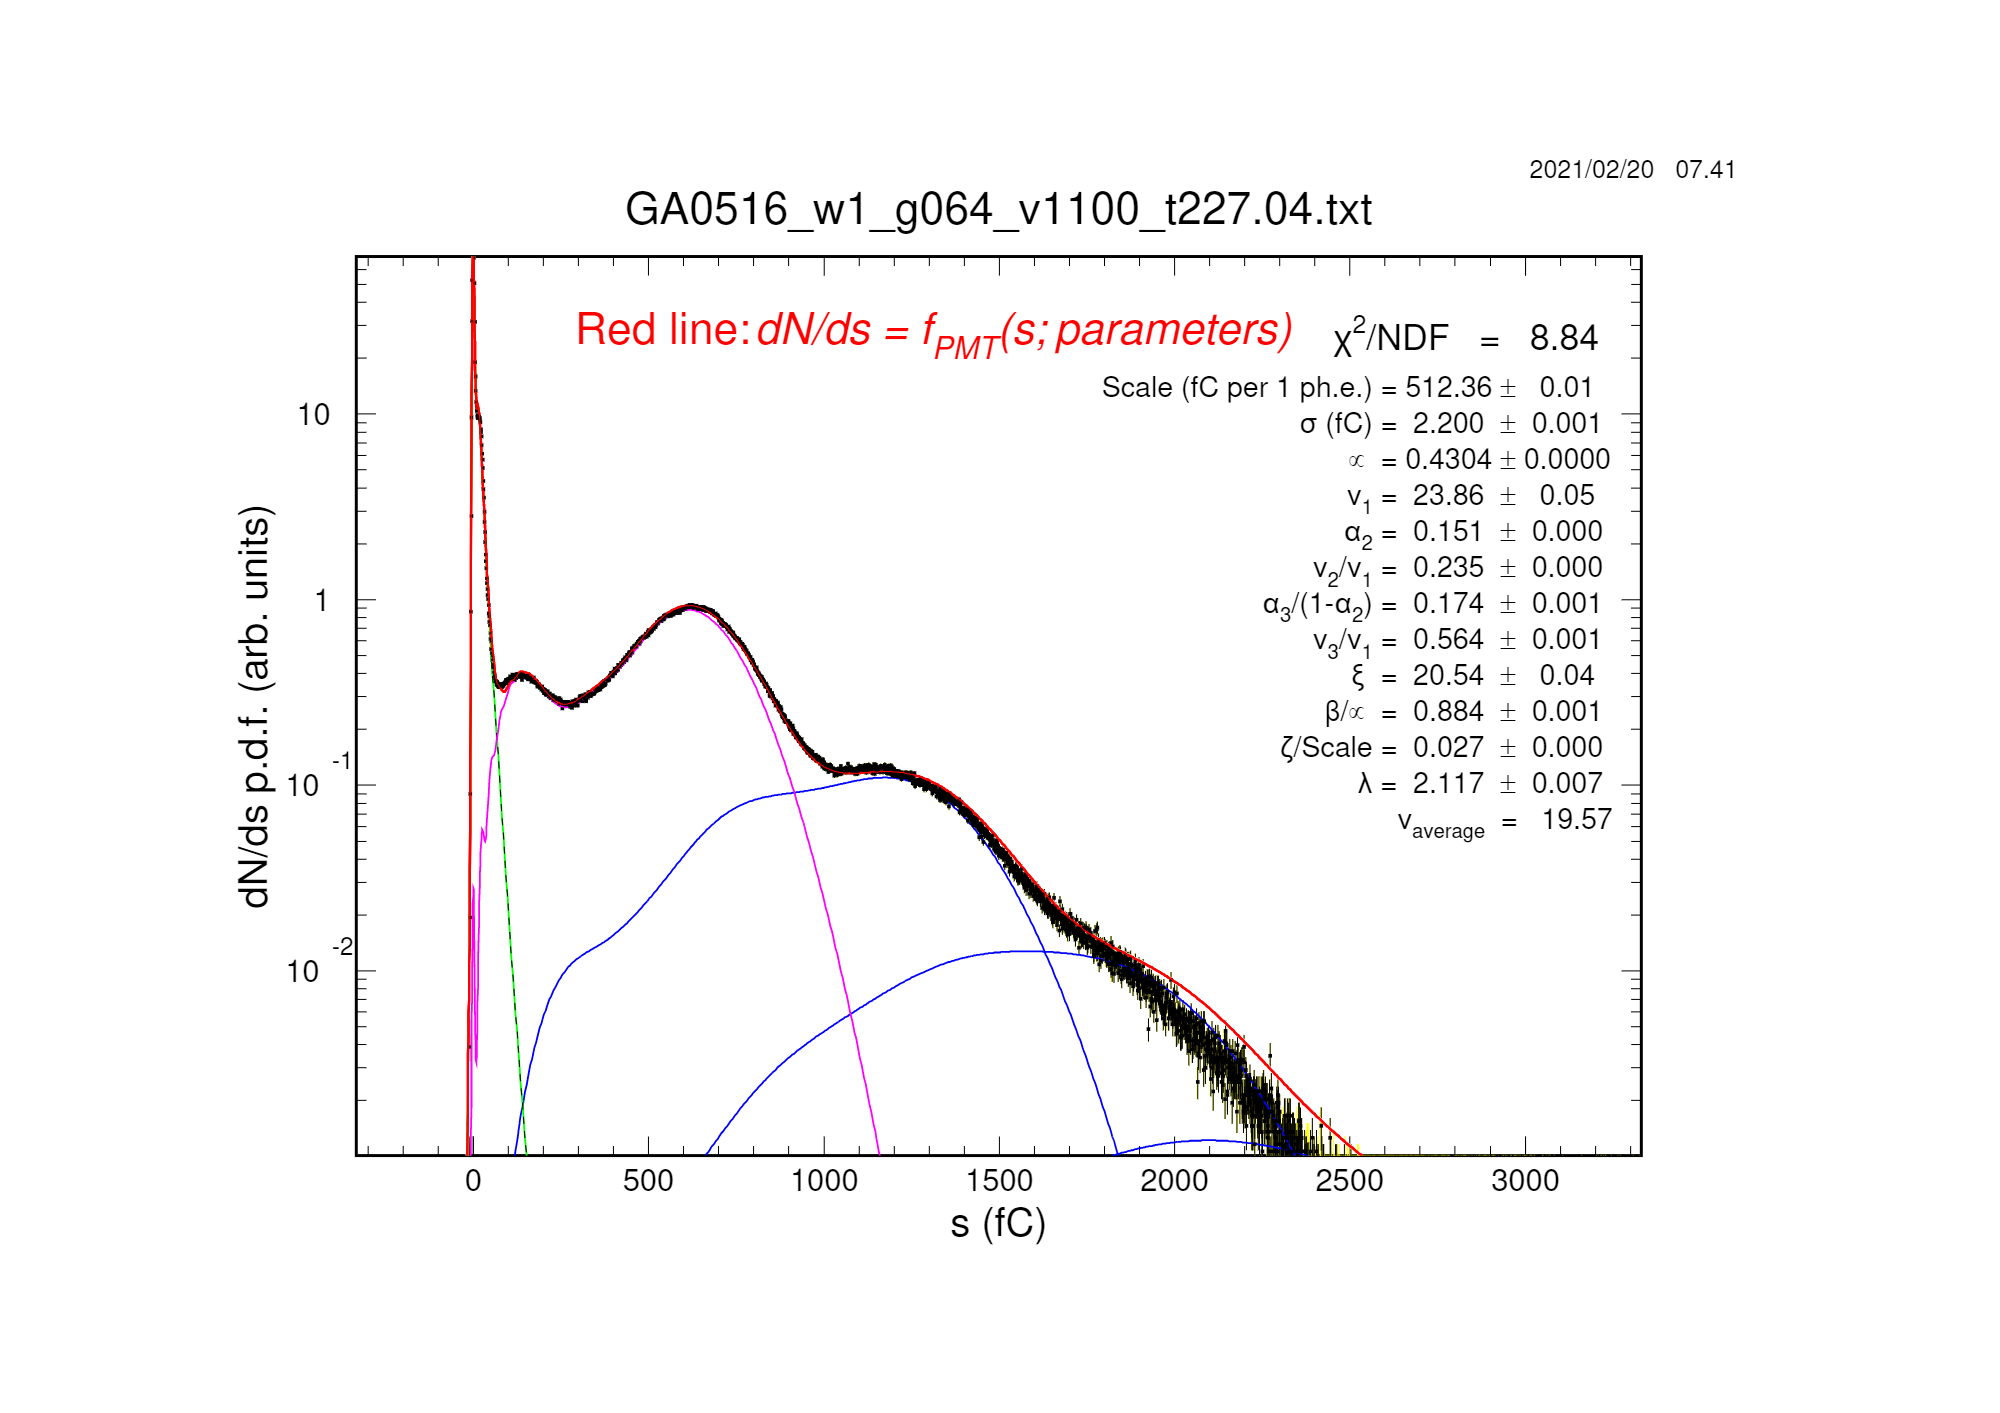
\includegraphics[width=\linewidth, trim={75mm 6cm 6cm 85mm},clip]{figures/GA0516_w1_g064_v1100_raw_log.04.png}
		\vspace{0mm}
	\end{subfigure}%%
	\caption{Same as Fig.~\ref{fig:GA0516_w2_fits} but at the wheel position 1.}
	\label{fig:GA0516_w1_fits}
\end{figure*}

\begin{figure*}
	\centering
	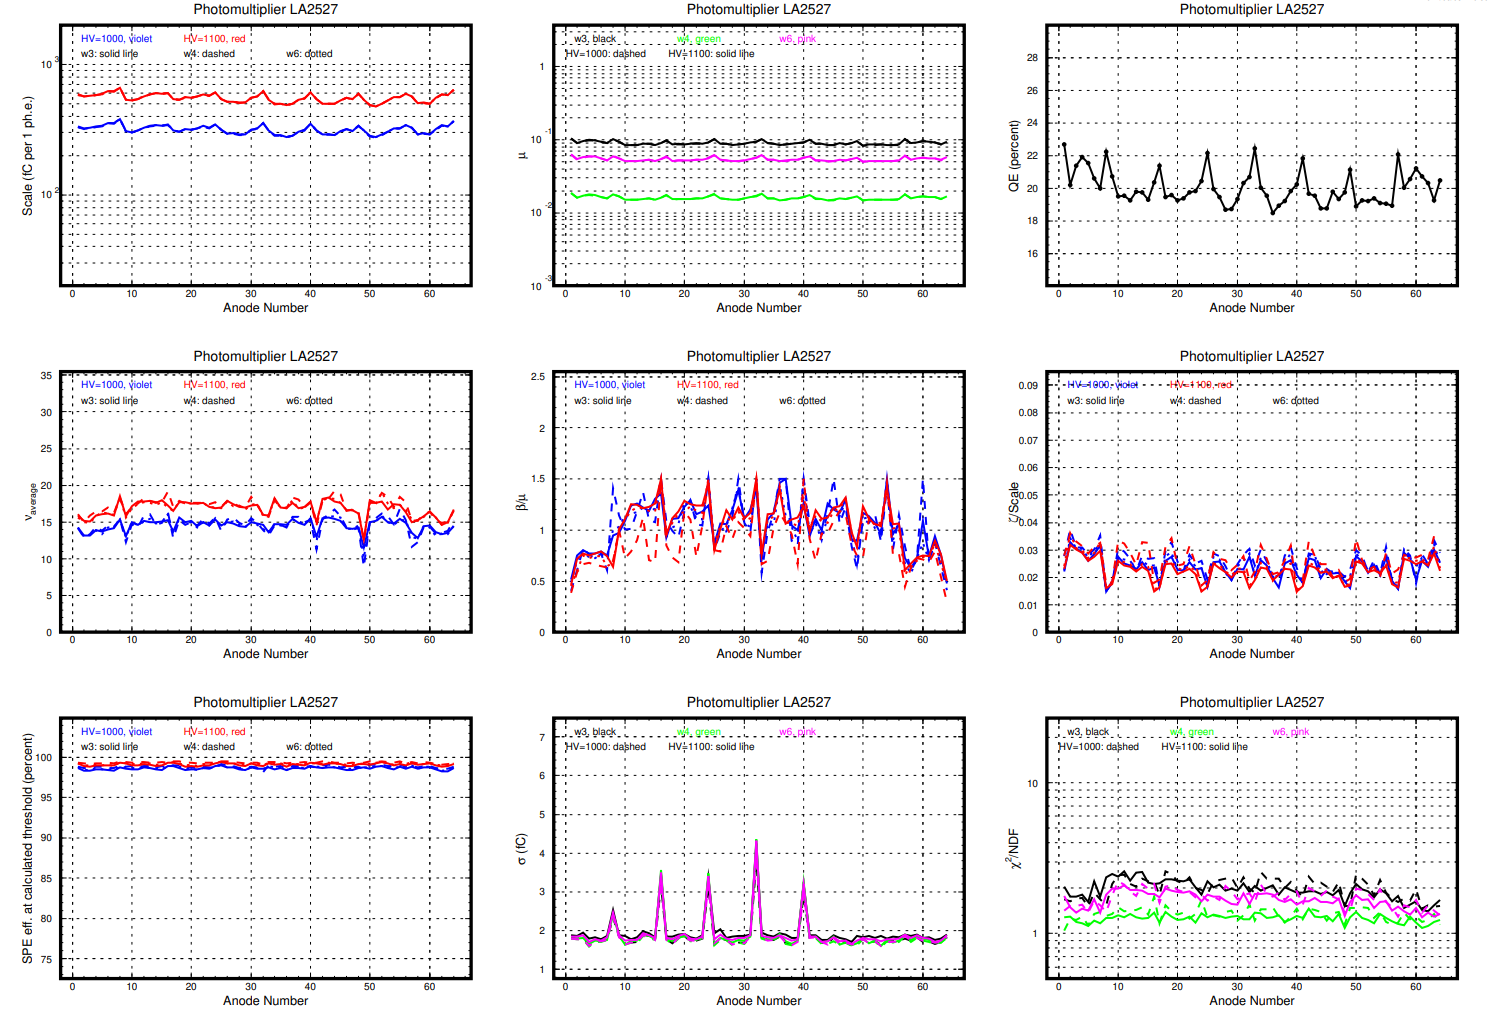
\includegraphics[width=0.85\textwidth]{figures/pavel_temp/LA2527_passport_temp.png}
	\caption{Illustration of the "PSPMT Passport" plots for one of the tubes, LA2527. The standard six measurements included runs at three illumination settings (wheel positions 3, 4, and 6), each at two operating high voltage values (1000 V, and 1100 V).}
	\label{fig:LA2527_passport}
\end{figure*}


\begin{figure*}
	\centering
	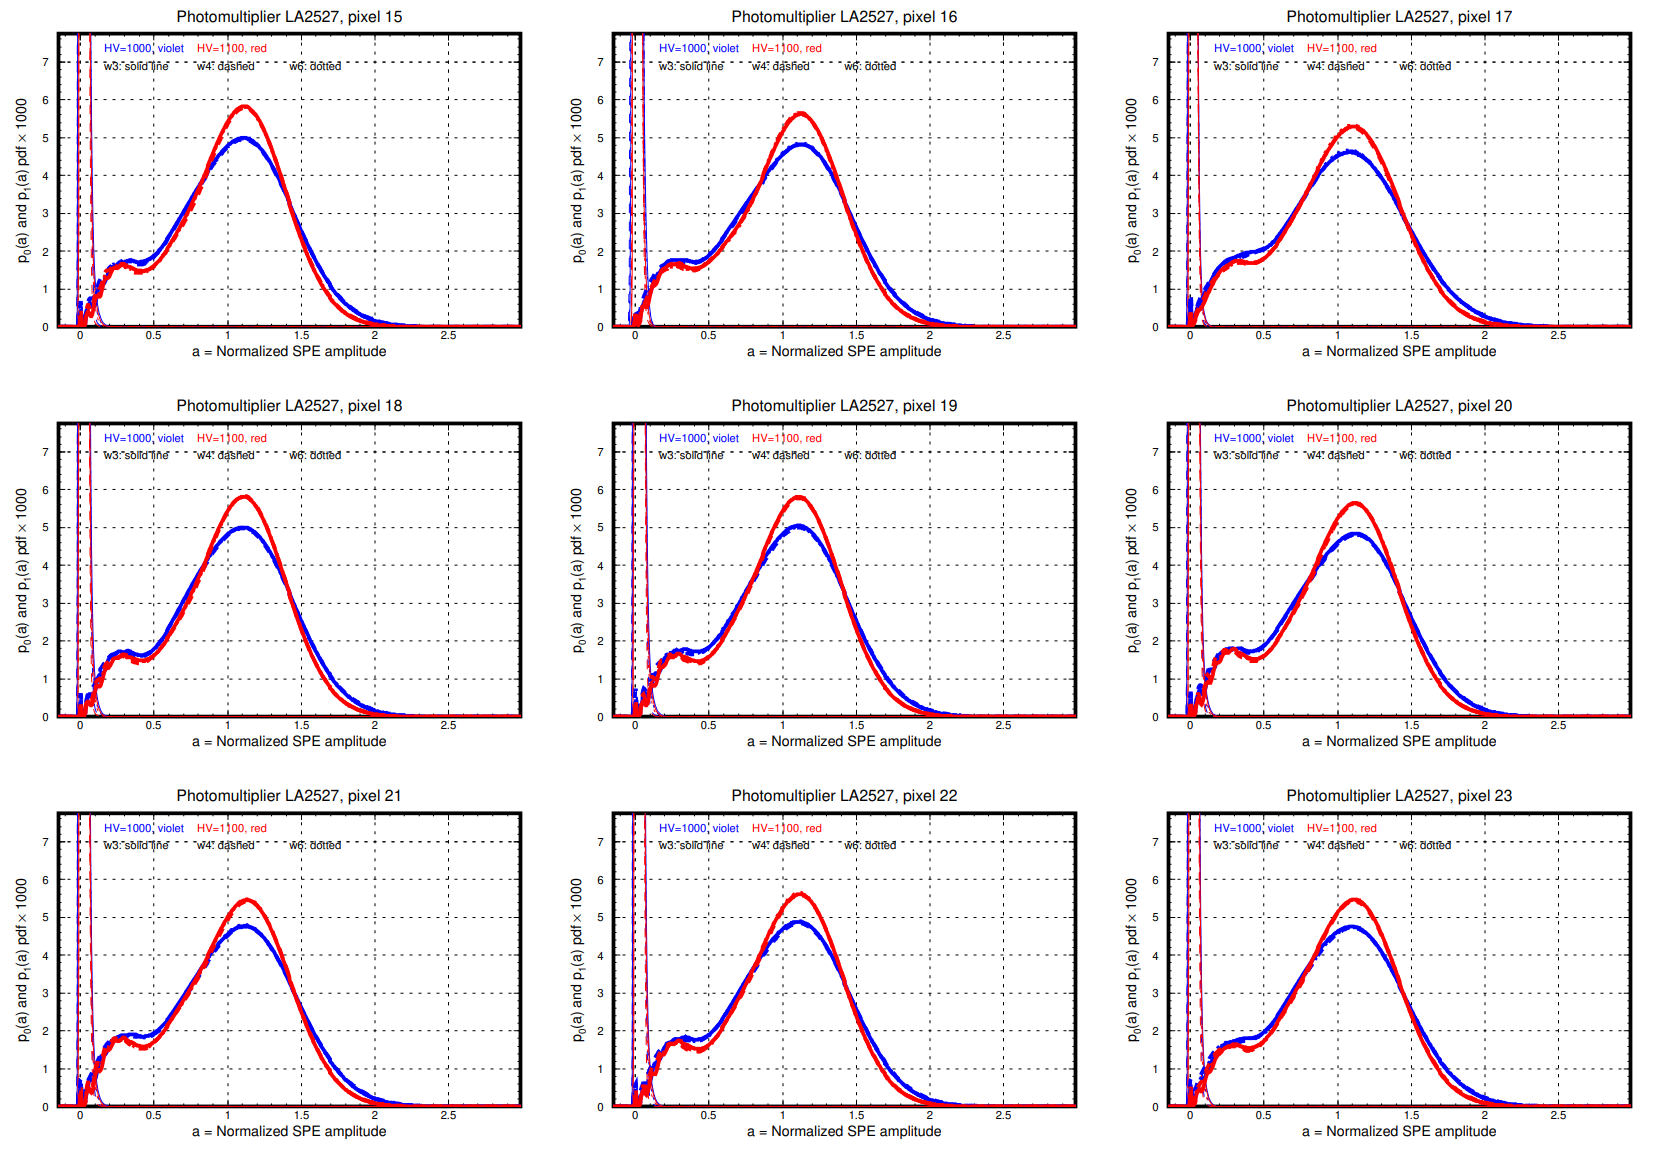
\includegraphics[width=0.85\textwidth]{figures/pavel_temp/LA2527_spectra_temp.png}
	\caption{Illustration of the "PSPMT Passport" plots for one of the tubes, LA2527, continued. The standard six measurements included runs at three illumination settings (wheel positions 3, 4, and 6), each at two operating high voltages (1000 V, and 1100 V). Shown are the calculated SPE functions, defined by the fit parameters resulting from the independent fitting procedures for each six settings. Blue color corresponds to the three sets at HV = 1000 V, and red - to the runs at HV = 1100 V. The fit parameters of the independent fits at three different illuminations result in very stable SPE shapes, essentially overlapping each other in the plots.}
	\label{fig:LA2527_passport_spectra}
\end{figure*}

\begin{figure}
	\centering
	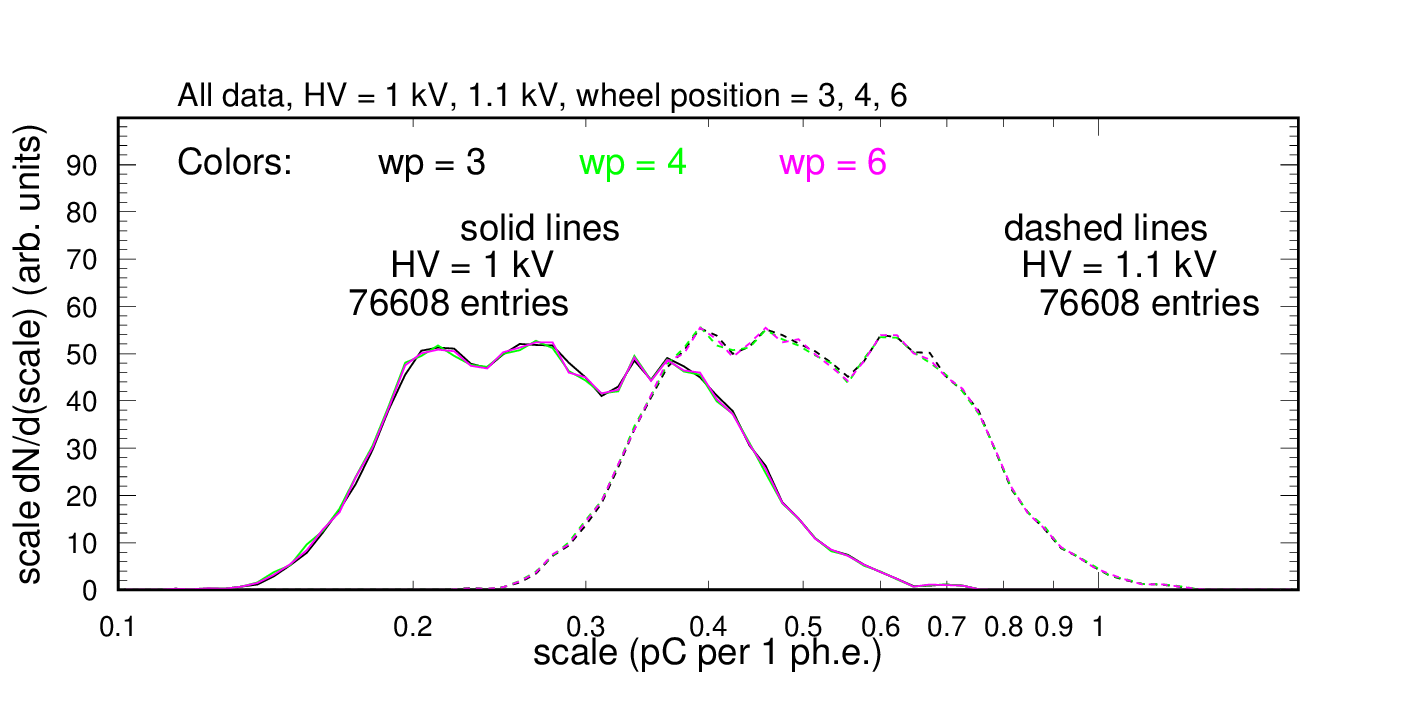
\includegraphics[width=0.95\linewidth]{figures/pglobal_sc.pdf}
	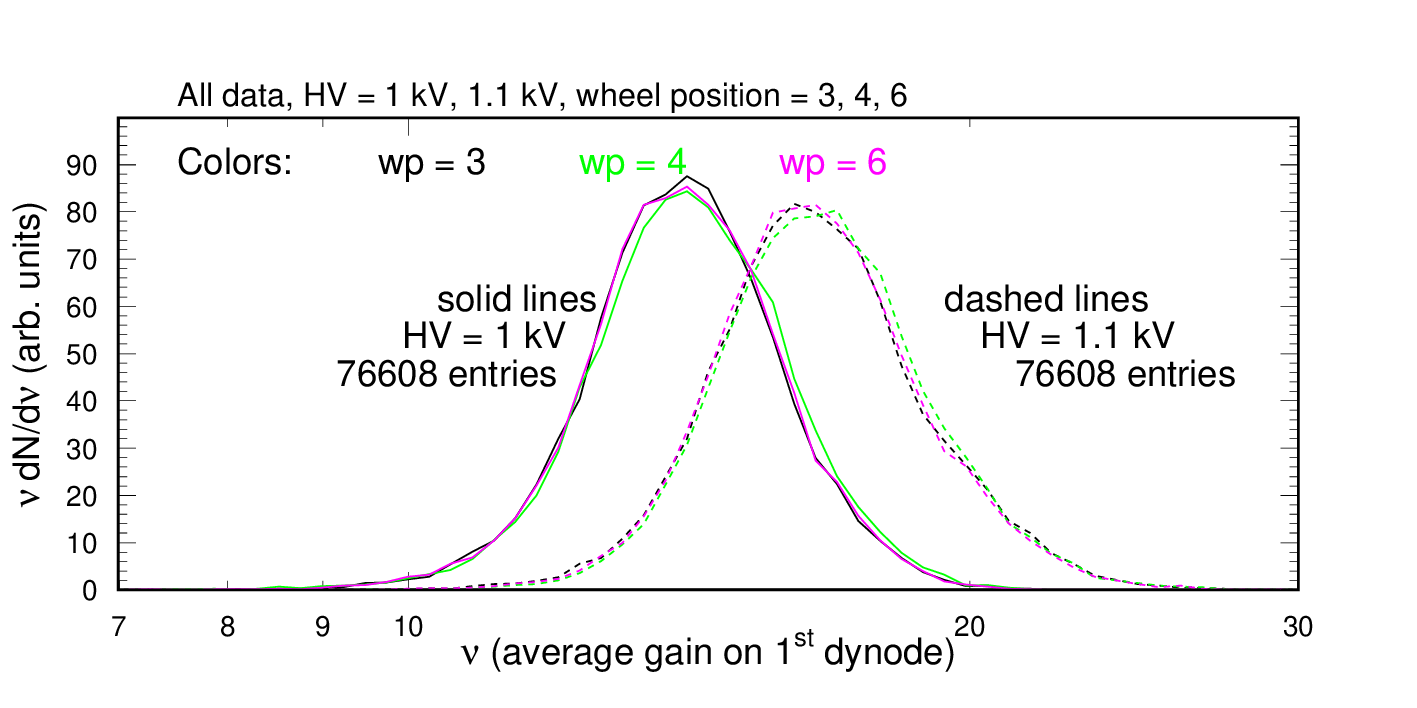
\includegraphics[width=0.95\linewidth, trim={0mm 0mm 0mm 19mm}, clip]{figures/pglobal_nu.pdf}
	\caption{Distribution of scale (average charge per ph.e) and $\nu$ (average gain on 1st dynode) as determined by the fitting procedure for a set of 399 PMTs.}
	\label{fig:pglobal_sc_nu}
\end{figure}

\begin{figure}
	\centering
	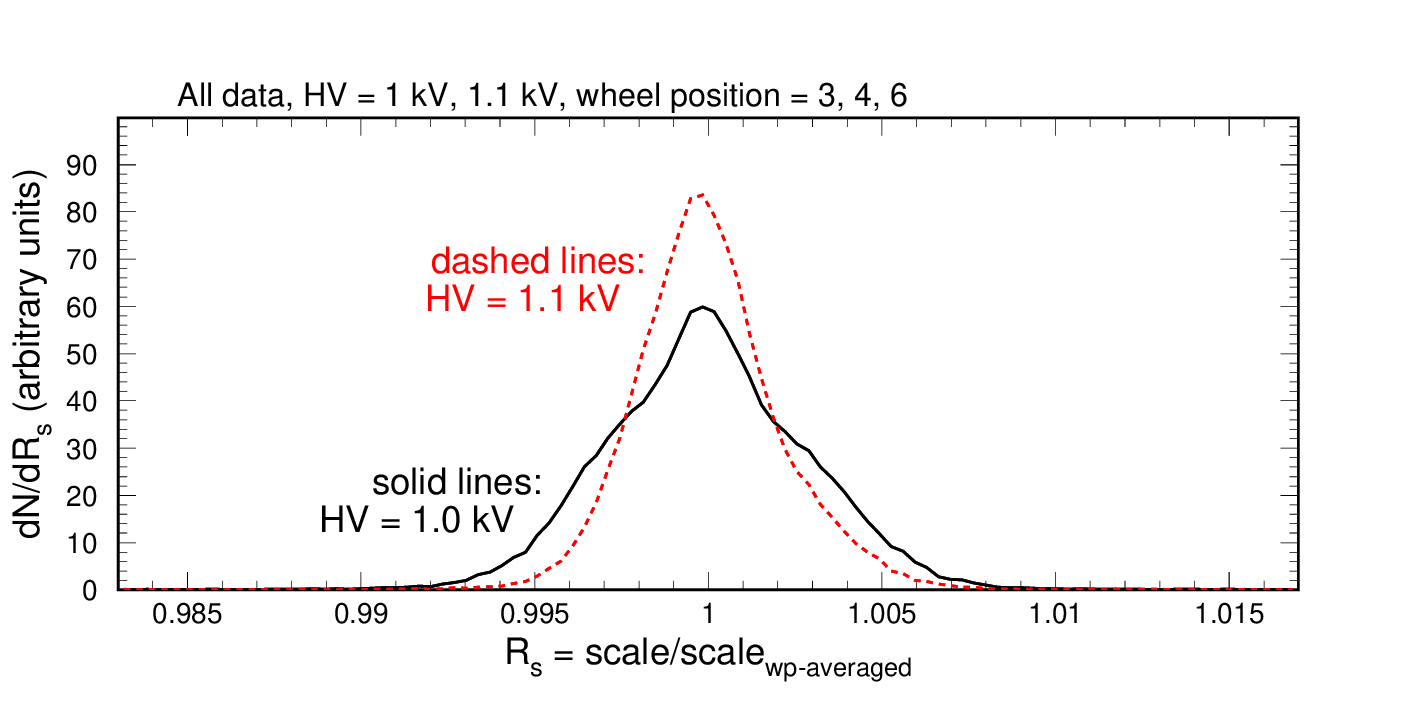
\includegraphics[width=0.95\linewidth]{figures/pglobal_Rs.pdf}
	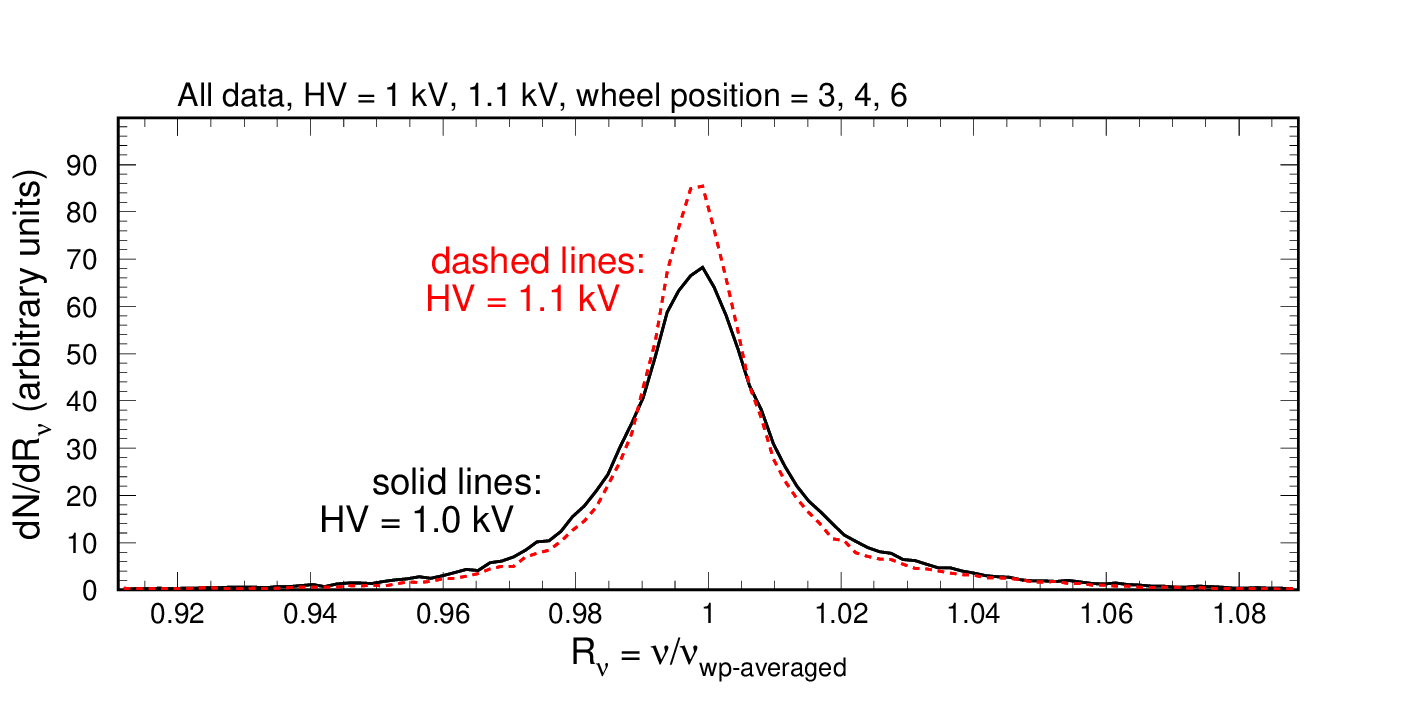
\includegraphics[width=0.95\linewidth, trim={0mm 0mm 0mm 19mm}, clip]{figures/pglobal_Rn.pdf}
	\caption{Scale and $\nu$ averaged over three different illumination settings (wheel positions 3, 4, and 6).}
	\label{fig:pglobal_Rs_Rn}
\end{figure}

\begin{figure}
	\centering
	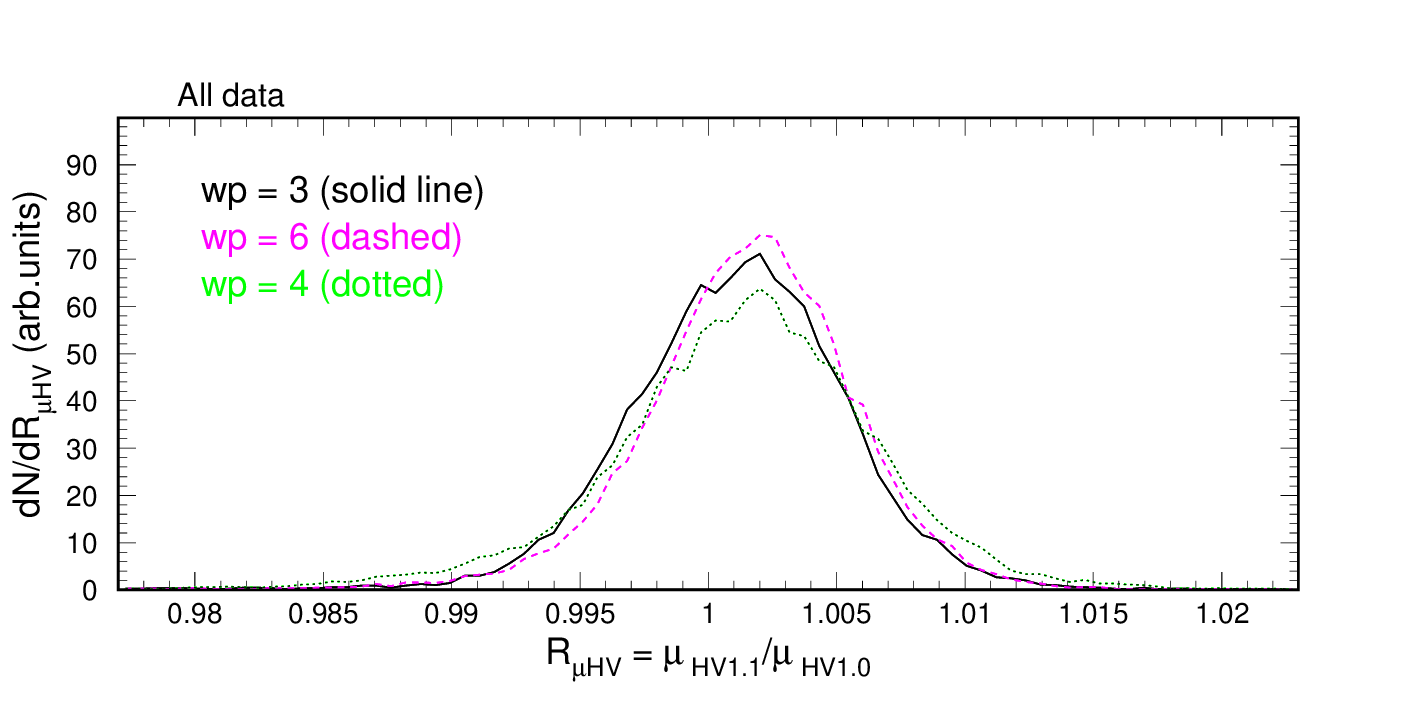
\includegraphics[width=0.95\linewidth]{figures/pglobal_mHV.pdf}
	\caption{The ratio of the $\mu$ parameters from the fit results at HV = 1100 V to the results at HV = 1000 V.}
	\label{fig:pglobal_mHV}
\end{figure}


\begin{figure}
	\centering
	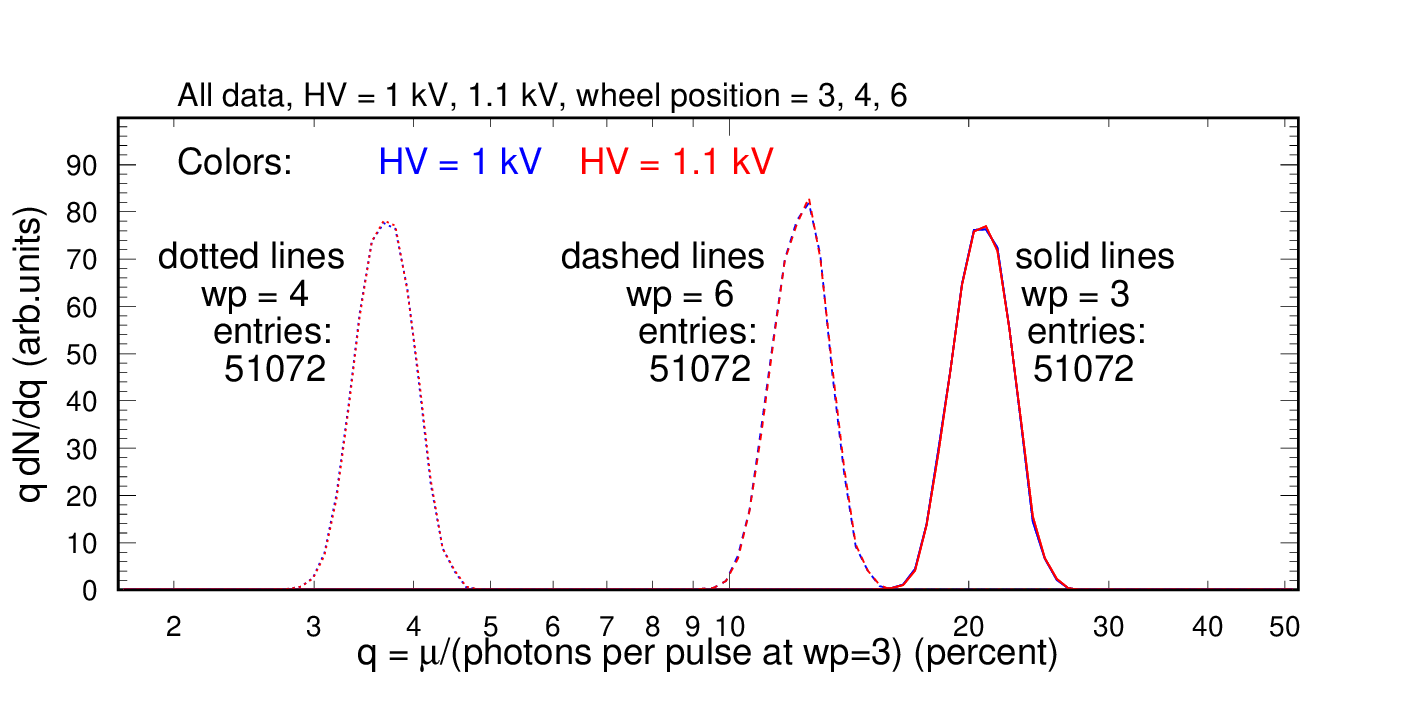
\includegraphics[width=0.95\linewidth]{figures/pglobal_qe_all.pdf}
	\caption{Distribution of $\mu$ divided by the measured number of photons per pulse at wheel position 3. For the data collected at wheel position 3, this ratio is the quantum efficiency of the individual pixels.}
	\label{fig:pglobal_qe_all}
\end{figure}

\begin{figure}
	\centering
	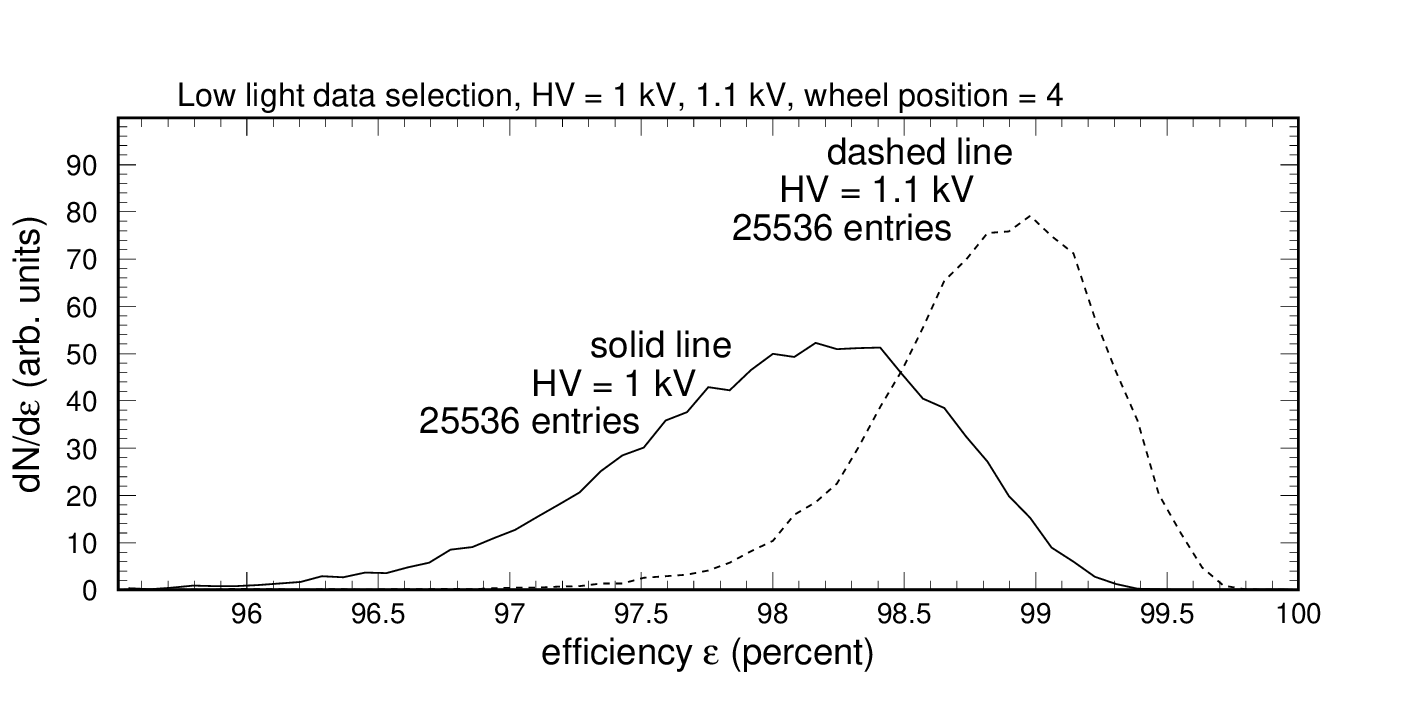
\includegraphics[width=0.95\linewidth]{figures/pglobal_eff.pdf}
	\caption{Distribution of the measured efficiency for all pixels at wheel position 4.}
	\label{fig:pglobal_eff}
\end{figure}

\begin{figure}
	\centering
	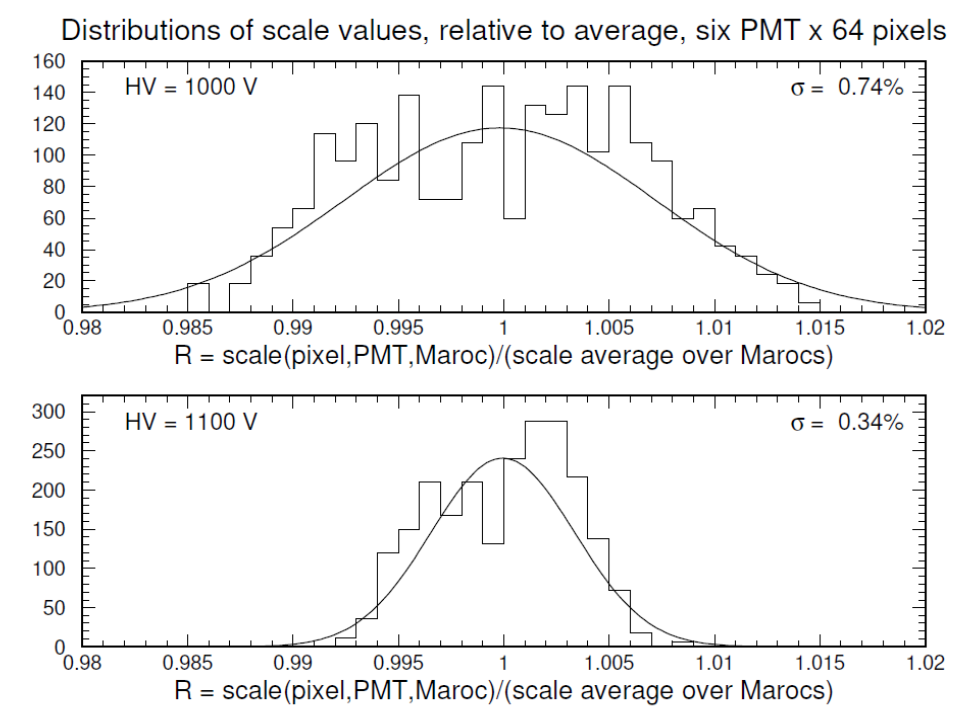
\includegraphics[width=0.95\linewidth]{figures/R_scale_maroc_avg.png}
	\caption{Evaluated precision of the scale parameter measurement for the two high voltage settings.}
	\label{fig:R_scale_maroc_avg}
\end{figure}


\begin{figure*}[b]
	\centering
	\begin{subfigure}[c]{0.4\linewidth}
		\centering
		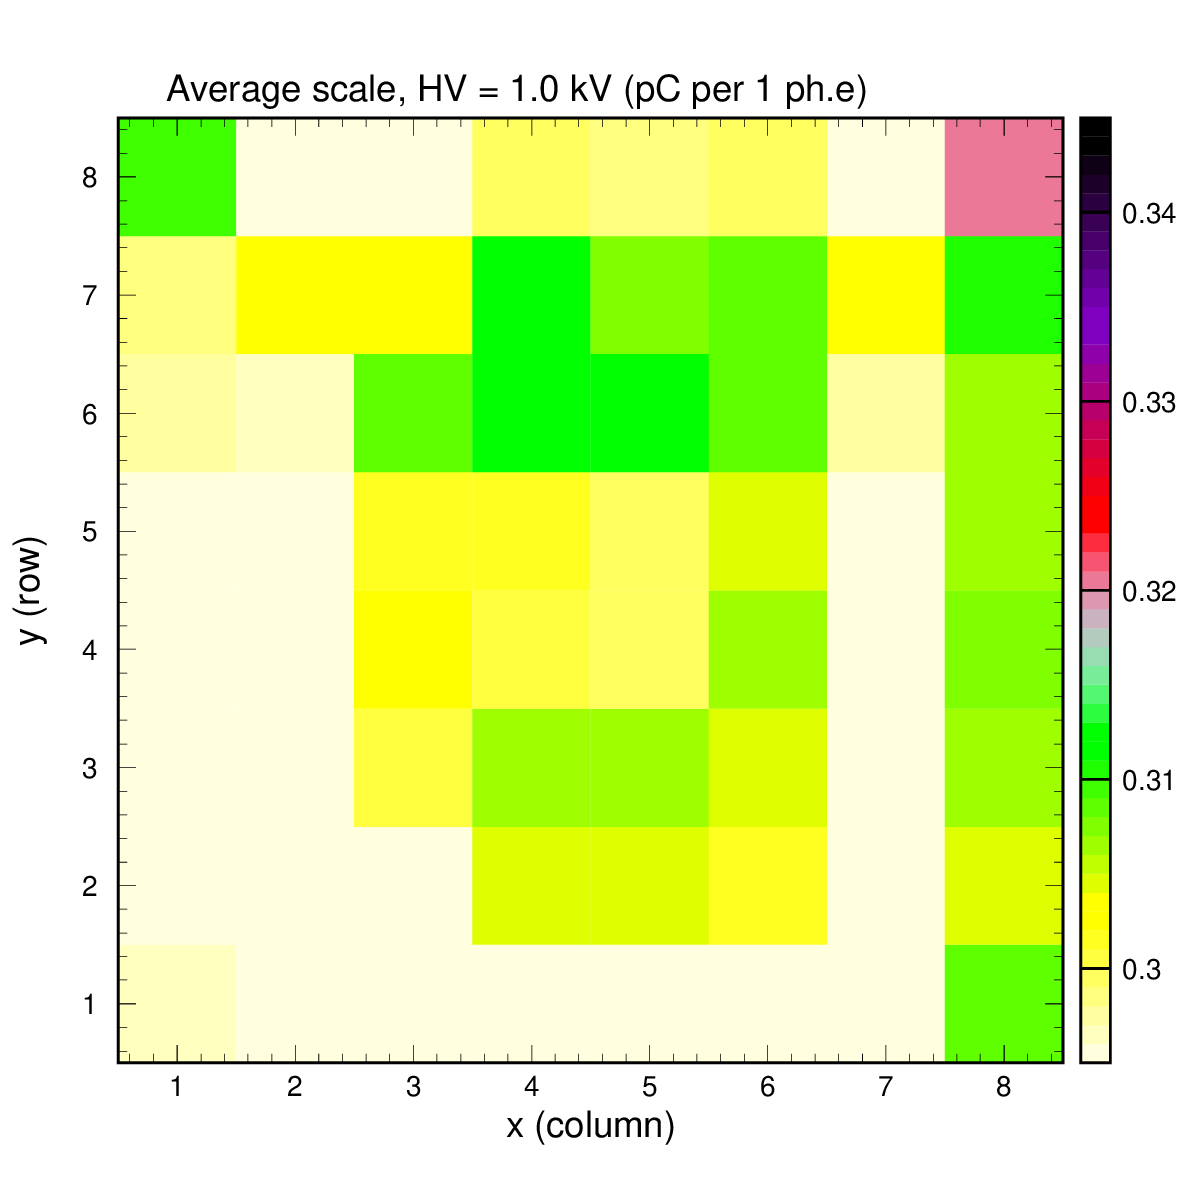
\includegraphics[width=\linewidth, trim={0mm 0mm 0mm 19mm},clip]{figures/pglobal_sc2d.pdf}
		\caption{Average scale, HV = 1.0 kV (pC per 1 ph.e)}
		\vspace{0mm}
	\end{subfigure}%%
	\begin{subfigure}[c]{0.4\linewidth}
		\centering
		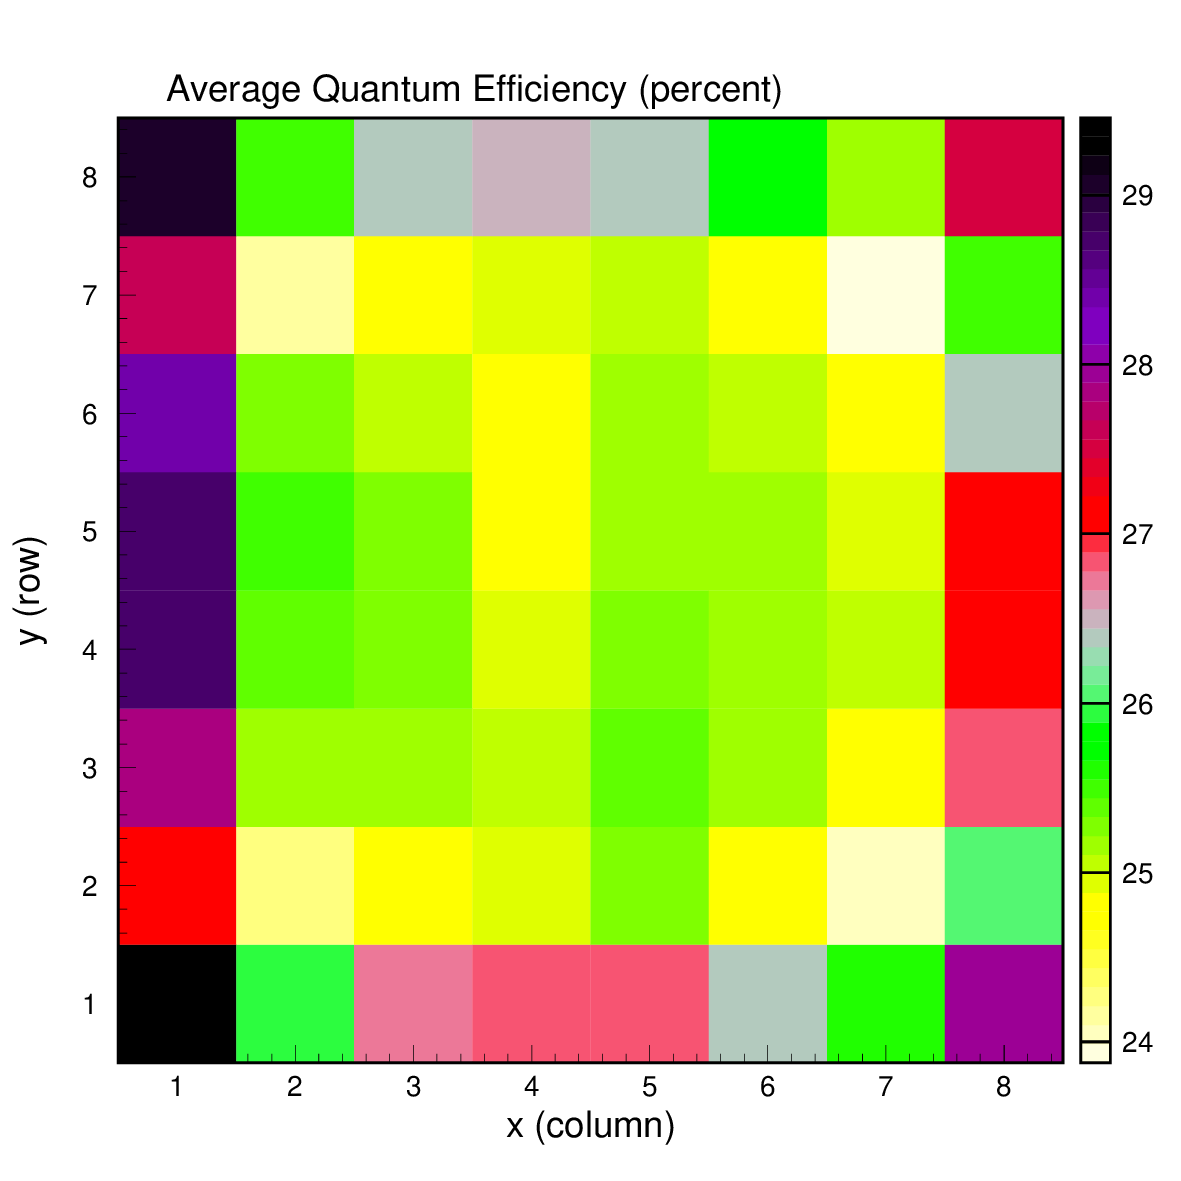
\includegraphics[width=\linewidth, trim={0mm 0mm 0mm 19mm},clip]{figures/pglobal_qe.pdf}
		\caption{Average Quantum Efficiency (percent)}
		\vspace{0mm}
	\end{subfigure}%%
	\vspace{3mm}
	\begin{subfigure}[c]{0.4\linewidth}
		\centering
		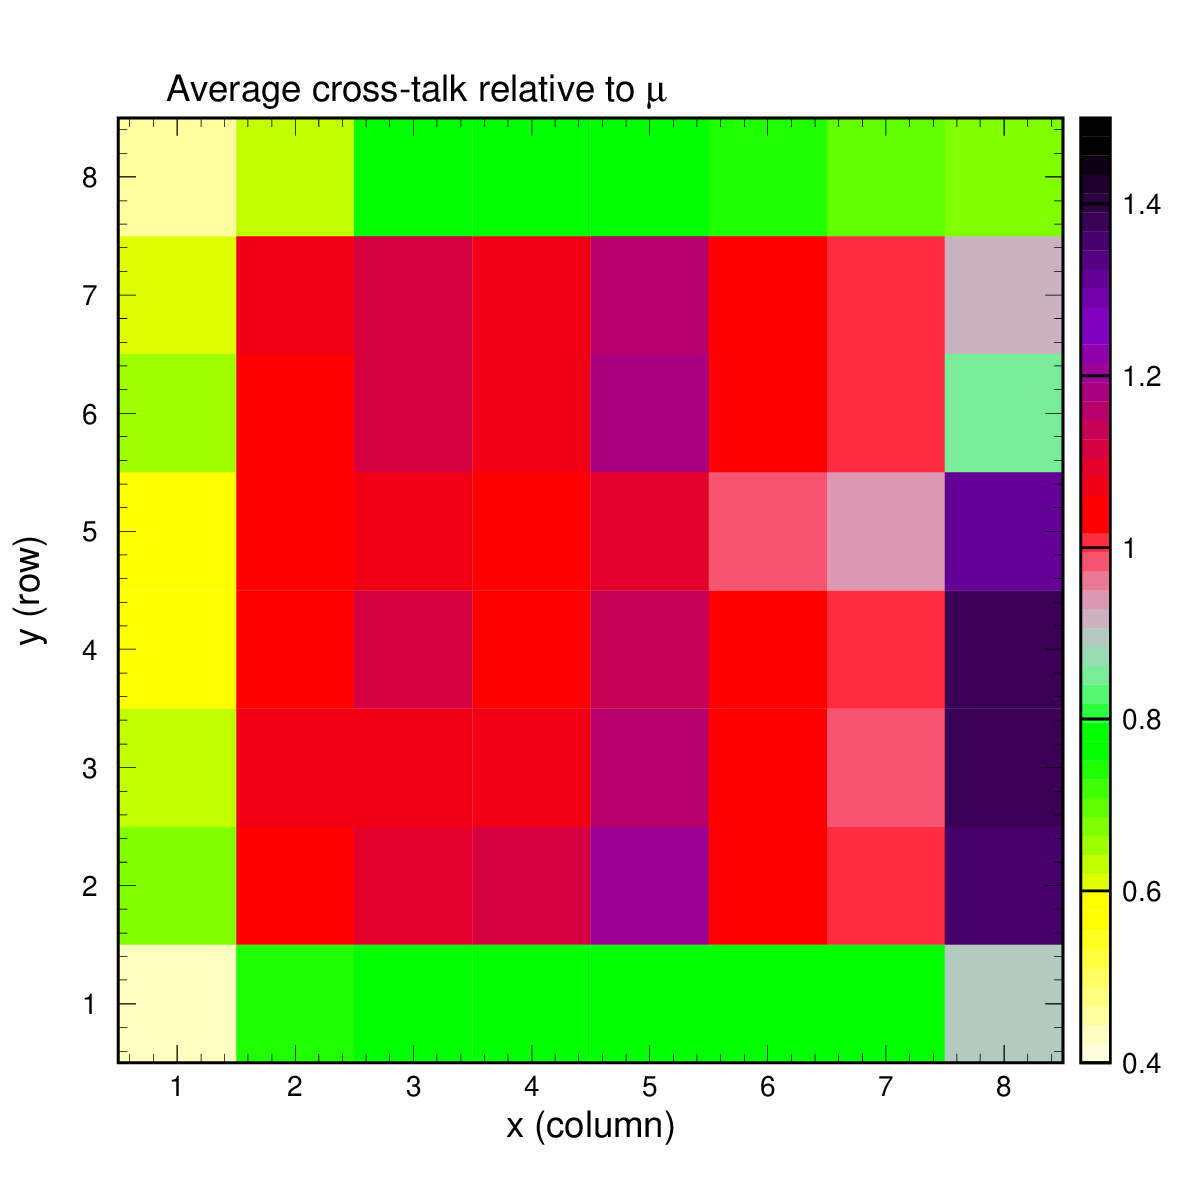
\includegraphics[width=\linewidth, trim={0mm 0mm 0mm 19mm},clip]{figures/pglobal_beta.pdf}
		\caption{Average cross-talk relative to $\mu$}
		\vspace{0mm}
	\end{subfigure}%%
	\begin{subfigure}[c]{0.4\linewidth}
		\centering
		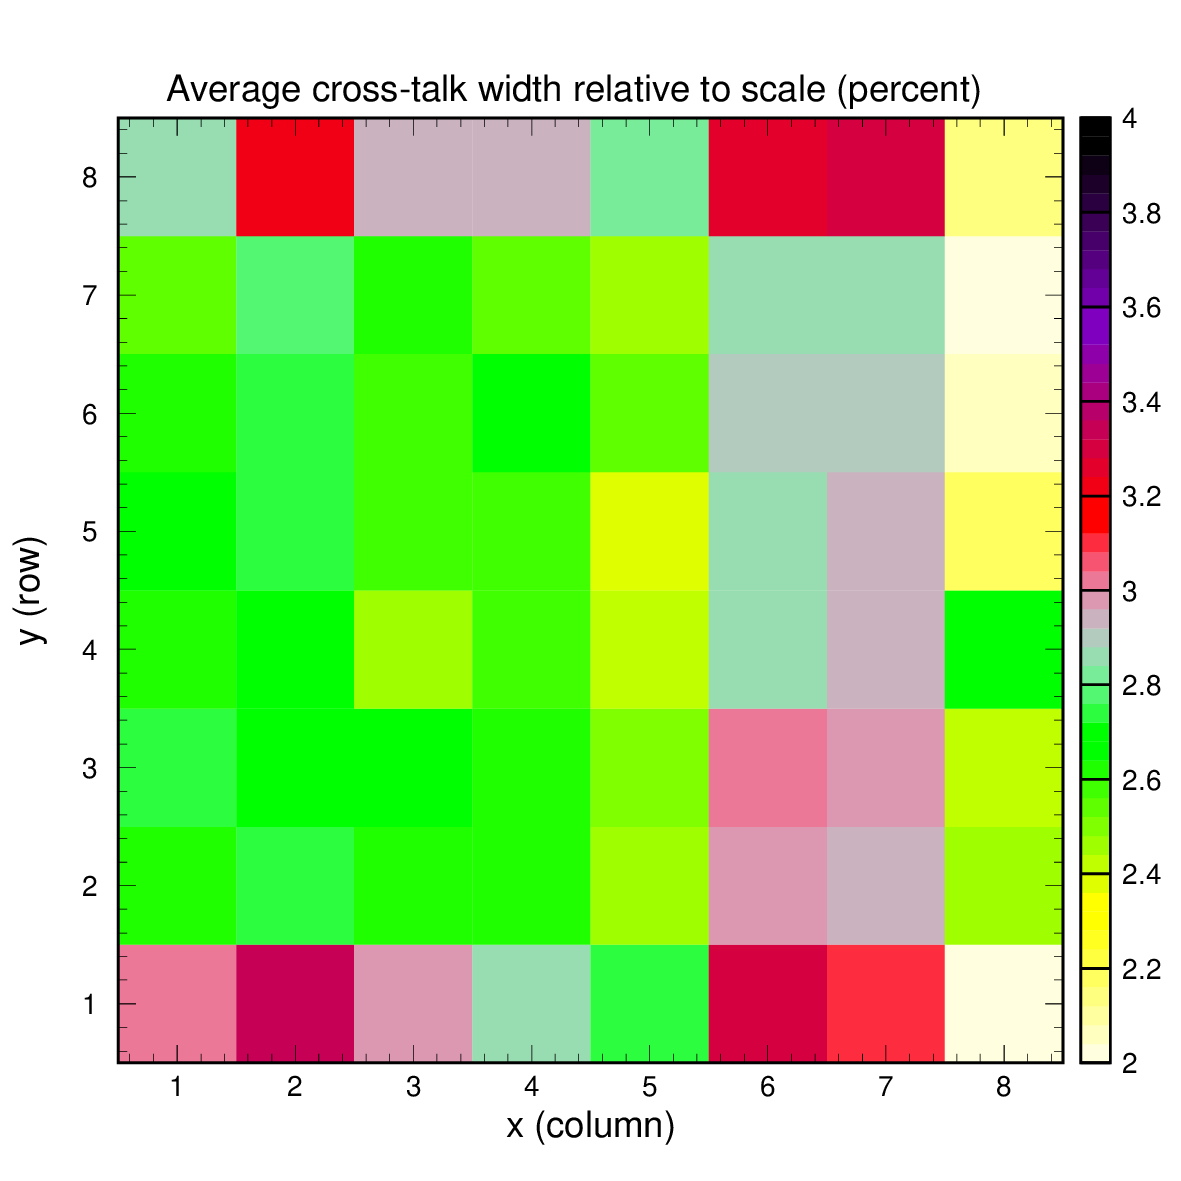
\includegraphics[width=\linewidth, trim={0mm 0mm 0mm 19mm},clip]{figures/pglobal_zeta.pdf}
		\caption{Average cross-talk width relative to scale (percent)}
		\vspace{0mm}
	\end{subfigure}%%
	\vspace{3mm}
	\begin{subfigure}[c]{0.4\linewidth}
		\centering
		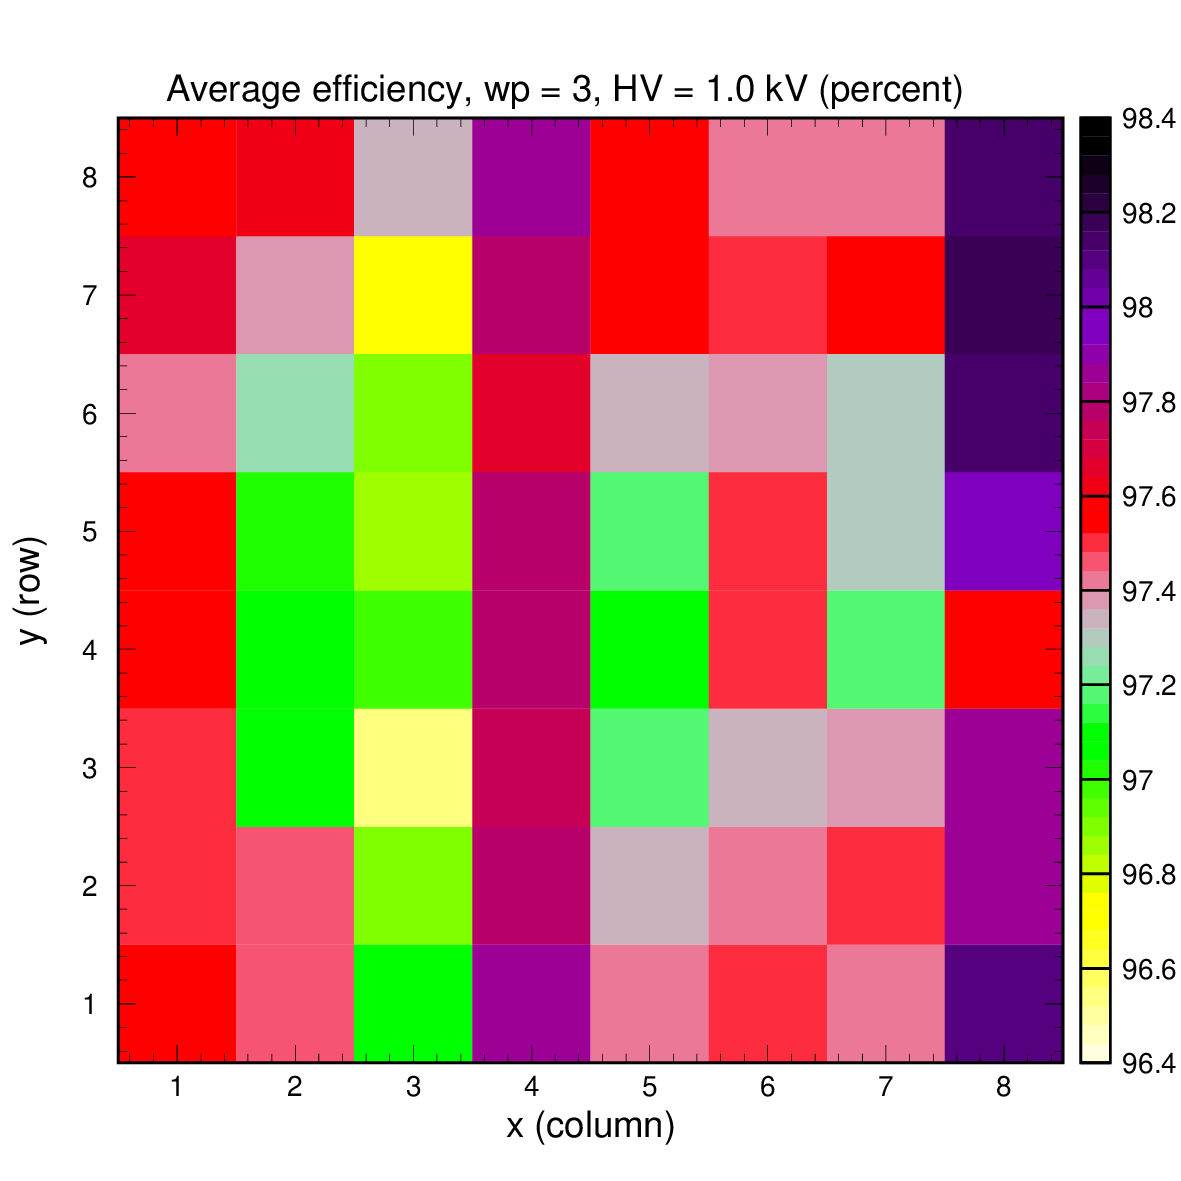
\includegraphics[width=\linewidth, trim={0mm 0mm 0mm 19mm},clip]{figures/pglobal_eff2d.pdf}
		\caption{Average efficiency, wp = 3, HV = 1.0 kV (percent)}
		\vspace{0mm}
	\end{subfigure}%%
	\caption{Two dimensional plots showing the average (a) scale, (b) quantum efficiency, (c) cross-talk relative to $\mu$, (d) cross-talk relative to scale, and (e) efficiency as a function of pixel location.}
	\label{fig:2d_avg_fit_results}
\end{figure*}


%We saw that although there is little difference in crosstalk signals, the H12700 PMTs suffer less from dark current, have narrower SPE spectra, and have higher $\mu$ and relative efficiency values.
%An example plot of the $\mu$'s and relative efficiencies of H8500 and H12700 PMTs with similar low and high gains is shown in Figure \ref{efficiency}.

%We see that the relative efficiency is closely related to the $\mu$ which is on average, over all pixels at all voltages for all the PMTs we tested, $29\pm5$ percent higher in H12700 than H8500 MAPMTs. One concern with these $\mu$ measurements however is that the laser system used to measure these PMTs was only incident on a portion of each pixel, consequently missing their sum total effect and pinpointing possible spatial dependencies which should be further studied and perhaps remeasured with a fully illuminated MAPMT instead of collimated pinpoint laser light. In terms of crosstalk for the two varieties of MAPMT the H12700s appear to be better than the H8500s. The H12700s have a decrease in crosstalk by nearly a factor of two. Additional studies of dark current in the H12700s would be useful, as the dark current is usually dominated by individual pixels or bad regions of the PMT instead of spread around evenly like in the H8500s, but overall the two varieties are not very different in terms of dark current.